%% =====================================================================
%%  ARTICLE 4 (working skeleton)
%%
%%  Coarse Observability Across High-Order Finite-Volume
%%  Reconstructions: Universal Rank, Conditioning, and
%%  Dissipative Memory
%%  (title adopted 2026-08-24 from revision report 1, item P3)
%%
%%  Target journal : Advances in Computational Mathematics (Springer)
%%                   (retargeted 2026-08-24 from J. Sci. Comput., item P4)
%%  Document class : sn-jnl (Springer Nature), sn-mathphys-num style
%%                   (class + .bst shipped locally, as in the FVerasure package)
%%
%%  Related manuscripts (cited as prior/related work, not depended upon):
%%    [FVerasure] Exact Finite-Horizon Memory, Conditioning, and Dissipative
%%              Decay in Coarse Upwind Finite-Volume Prediction (JSC, submitted)
%%    [onestep] Initial-Trace Insufficiency and Entropy-Accounting Separation
%%              in Finite-Volume Coarse Graining (in preparation)
%%    [lifting] Exact Lifting of Coarse Histories in Periodic Upwind Finite
%%              Volumes (short note; source in companion_articles/paper_C/)
%%
%%  Skeleton conventions:
%%    - \todo{...} marks work to be done (renders red in the PDF).
%%    - "Target Theorem/Conjecture" = result to be proved during drafting;
%%      stated precisely so the numerical campaign can test it as-is.
%%    - Figure/table filenames match the planned reproducibility repo layout
%%      (figures/*.pdf, results/*.csv, tables/*.tex), as in the FVerasure package.
%% =====================================================================

\documentclass[pdflatex,sn-mathphys-num]{sn-jnl}% Math and Physical Sciences Numbered Reference Style

%%---------------- Packages (mirrors the FVerasure known-good preamble) ----------------
\usepackage{graphicx}%
\usepackage{amsmath,amssymb,amsfonts}%
\usepackage{amsthm}%
\usepackage[title]{appendix}%
\usepackage{xcolor}%
\usepackage{booktabs}%
\usepackage{array}%
\usepackage{csquotes}

\makeatletter
\@ifpackageloaded{geometry}%
  {\geometry{a4paper,margin=1in}}%
  {\usepackage[a4paper,margin=1in]{geometry}}
\makeatother
\usepackage{mathtools}
\usepackage{subcaption}
\usepackage{bookmark}
\usepackage{microtype}
% sn-jnl.cls ships an EPS-based \orcidlogo (Orcidlogo.eps, not included
% in the distribution); undefine it so the self-contained TikZ version
% of the "orcidlink" package can take over.
\let\orcidlogo\undefined
\usepackage{orcidlink}
\usepackage[numbers,sort&compress]{natbib}
\makeatletter
\@ifpackageloaded{hyperref}%
  {\hypersetup{colorlinks=true,linkcolor=blue,citecolor=blue,urlcolor=blue,pdftitle={Coarse Observability Across High-Order Finite-Volume Reconstructions: Universal Rank, Conditioning, and Dissipative Memory},pdfauthor={Antonis Polemitis, Ioannis Kokkinakis, Nicholas Christakis, Dimitris Drikakis},}}%
  {\usepackage[colorlinks=true,linkcolor=blue,citecolor=blue,urlcolor=blue]{hyperref}\hypersetup{pdftitle={Coarse Observability Across High-Order Finite-Volume Reconstructions: Universal Rank, Conditioning, and Dissipative Memory},pdfauthor={Antonis Polemitis, Ioannis Kokkinakis, Nicholas Christakis, Dimitris Drikakis},}}
\makeatother
\usepackage[nameinlink]{cleveref}
\crefname{conjecture}{conjecture}{conjectures}

%%---------------- Theorem environments (sn-jnl styles) ----------------
\theoremstyle{thmstyleone}%
\newtheorem{theorem}{Theorem}%
\newtheorem{lemma}{Lemma}%
\newtheorem{proposition}{Proposition}%
\newtheorem{corollary}{Corollary}%
\newtheorem{conjecture}{Conjecture}%

\theoremstyle{thmstyletwo}%
\newtheorem{remark}{Remark}%
\newtheorem{example}{Example}%

\theoremstyle{thmstylethree}%
\newtheorem{definition}{Definition}%

%%---------------- Macros ----------------
\newcommand{\R}{\mathbb R}
\newcommand{\epsmach}{\epsilon_{\rm mach}}
\DeclareMathOperator{\rank}{rank}
\DeclareMathOperator{\diag}{diag}
\DeclareMathOperator{\TV}{TV}
\DeclareMathOperator{\card}{card}
\newcommand{\OL}{{\cal O}_L}
\newcommand{\Asch}{A^{[\rm sch]}_\lambda}

%% Red TODO marker for the drafting phase.
\newcommand{\todo}[1]{\textcolor{red}{\textbf{[TODO: #1]}}}

\raggedbottom

\begin{document}

\title[Coarse Observability Across High-Order Reconstructions]{Coarse Observability Across High-Order Finite-Volume Reconstructions: Universal Rank, Conditioning, and Dissipative Memory}

\author[1]{\fnm{Antonis} \sur{Polemitis}\,\orcidlink{0000-0003-3188-8746}}\email{polemitis.an@unic.ac.cy}

\author*[2]{\fnm{Ioannis} \sur{Kokkinakis}\,\orcidlink{0000-0001-9694-3764}}\email{kokkinakis.i@unic.ac.cy}

\author*[2]{\fnm{Nicholas} \sur{Christakis}\,\orcidlink{0000-0001-9212-2336}}\email{christakis.n@unic.ac.cy}

\author[2]{\fnm{Dimitris} \sur{Drikakis}\,\orcidlink{0000-0002-3300-7669}}\email{drikakis.d@unic.ac.cy}

\affil[1]{\orgdiv{UNIC Evolve}, \orgname{University of Nicosia}, \city{Nicosia}, \postcode{CY-2417}, \country{Cyprus}}

\affil[2]{\orgdiv{Institute for Advanced Modelling and Simulation}, \orgname{University of Nicosia}, \city{Nicosia}, \postcode{CY-2417}, \country{Cyprus}}

\abstract{%
Coarse finite-volume averages are generally not a predictive state: exact coarse prediction requires additional memory whose dimension, recoverability, and lifetime were determined exactly in a recent study for first-order upwind advection.
This paper determines all three across the reconstruction hierarchy of practical computational fluid dynamics.
For linear circulant schemes --- Lax--Wendroff, Beam--Warming, Fromm, third- and fifth-order upwind-biased, and linear weighted-essentially-non-oscillatory (WENO) reconstructions --- we prove a universality theorem: outside a spectral-collision set, provably finite and certified empty for every operator and grid considered, the finite-horizon observation rank equals $P+(P-1)\min\{L,r-1\}$ --- the first-order upwind ladder, regardless of stencil width or formal order.
The proof exhibits an all-horizon invisible subspace and a universal depth-$r$ autonomous coarse recurrence, the scheme entering only through its coefficients.
Scheme dependence concentrates on three axes.
\emph{Timing}: in the single-parent regime, the exposure rate counts active stencil collars, not stencil width, and localized detection obeys a sharp reach-limited law.
\emph{Recoverability}: the smallest nonzero singular value of the single-parent observation map scales --- conjecturally for single-stage operators, with uniform numerical support --- as the Courant number raised to the exposure depth, so a second collar halves the conditioning exponent.
\emph{Relevance}: closed-form leading dissipation coefficients for the whole family give the erasure law $1-\rho_N\sim\tfrac12A(\lambda)(2\pi/N)^{2s}$: less-dissipative operators retain unresolved information orders of magnitude longer at identical memory dimension, and the fully discrete dissipative order belongs to the scheme--integrator pair.
For limited MUSCL and nonlinear WENO reconstructions, observability becomes state-dependent: on every affine limiter branch, the flux is exactly a linear blend, the active branch setting the local exposure rate, and collision ensembles at declared tolerances quantify the nonlinear residue --- including a plateau response-span staircase of approximately one direction per step across the tested amplitudes, beyond any linear budget.
For coarse-model validation, the centralized memory dimension is invariant across the collision-free linear hierarchy; detection timing, recovery conditioning, and dissipative lifetime must be declared with the scheme--integrator pair.}

\keywords{Finite-volume methods, High-order schemes, WENO, MUSCL, Coarse graining, Observability, Numerical dissipation}

\pacs[MSC Classification]{65M08, 65F35, 93B07, 65M12}

\maketitle

%% =====================================================================
\section{Introduction}\label{sec:intro}
%% =====================================================================

Finite-volume methods evolve cell averages through numerical fluxes at cell interfaces \cite{LeVeque2002,Toro2009,DrikakisRider2005}.
Whenever a fine computation is restricted, sampled, or replaced on a coarser grid, the same question arises: do the coarse cell averages alone contain enough information to predict their own future evolution?
In general, they do not --- a conservative restriction fixes how much material a parent cell holds but not where the material lies inside it, and the hidden placement determines when unresolved data reach parent interfaces and alter future coarse fluxes.
For first-order upwind advection on a periodic two-level hierarchy, a recent study \cite{PolemitisChristakisDrikakis2026FVerasure} made this deficit exact: it computed the dimension of the additional memory required for exact coarse prediction (a rank law with saturation at horizon $r-1$), the conditioning with which that memory can be recovered at a declared floating-point tolerance, and the rate at which numerical dissipation erases it.

However, first-order upwind is only the entry point.
Practical computational fluid dynamics (CFD) is built on high-resolution and high-order reconstructions --- flux-limited MUSCL schemes \cite{vanLeer1979,Harten1983,Sweby1984}, essentially non-oscillatory and weighted essentially non-oscillatory (WENO) reconstructions \cite{LiuOsherChan1994,JiangShu1996,Shu1998}, and wide upwind-biased linear stencils, usually paired with multistage time integrators \cite{GottliebShuTadmor2001}.
Every quantity in that analysis could, a priori, depend on the scheme, and the natural expectation runs in one direction: a stencil of reach $w$ transports information from $w$ cells per step, so hidden subcell data should become visible to the coarse observer roughly $w$ times faster, while the weaker numerical dissipation of high-order methods \cite{WarmingHyett1974,MargolinRider2002} should preserve that data longer.
If both effects held, high-order schemes would be doubly demanding for coarse closure --- more memory exposed per step, erased more slowly.

The first half of this expectation is false, and the failure is the main theorem of this paper.
For \emph{every} consistent linear circulant scheme --- outside a spectral-collision set that we prove finite and certify empty, in exact rational arithmetic, for all eight fully discrete operators and both grid pairs examined --- the finite-horizon observation rank equals $P+(P-1)\min\{L,r-1\}$: the first-order upwind ladder, independent of stencil width and formal order.
The saturation horizon, the invisible subspace, and the depth of the autonomous coarse recurrence are equally universal; a wider stencil cannot expose memory faster, because each observation step delivers only $P$ numbers, and one of them is redundant by conservation.
The scheme dependence is real, but it lives entirely on the other axes: \emph{when} localized hidden data are first detected (a sharp reach-limited law: the same compensated pair can stay geometrically shielded for five steps under first-order upwind and for none under the WENO5--SSP-RK3 pairing), \emph{how stably} the exposed directions can be recovered (conjecturally, with uniform numerical support: the conditioning exponent is the exposure depth, halved by a second active collar), and \emph{how long} they stay dynamically relevant (dissipative order $2s$ gives erasure in $\Theta(N^{2s})$ steps, spreading the information half-life across nearly five orders of magnitude at fixed resolution).
For nonlinear limited and WENO reconstructions, the observation object is no longer a fixed matrix; we prove that on every affine limiter branch the MUSCL flux is exactly a linear blend --- so the locally \emph{active branch} sets the exposure rate --- and quantify the genuinely nonlinear residue with ensembles of same-coarse-average collision pairs.

These four quantities are exactly those determined for first-order upwind in \cite{PolemitisChristakisDrikakis2026FVerasure, PolemitisChristakisDrikakis2026onestep}; each contribution below addresses one of them across the scheme hierarchy, under the same discipline: every claim is tied to a declared tolerance, every exact statement is backed by rational-arithmetic computation where feasible, and every figure and table is regenerated by a self-testing, dependency-light reproducibility package.
The scope is deliberately narrow, namely, linear scalar advection on a uniform periodic hierarchy, with empirical (ensemble-based) results for nonlinear schemes. The limitations are stated in \cref{sec:limitations}.

\subsection{Contributions}\label{sec:contributions}

\begin{enumerate}
\item \emph{Universality of the memory dimension} (\cref{thm:rank-universal,thm:invisible-general}): outside a spectral-collision set, provably finite (\cref{lem:collision-finite}) and certified empty on $(0,1]$ in exact rational arithmetic (\cref{prop:collision-empty,prop:collision-certificate}, E1b), $\rank\OL=P+(P-1)\min\{L,r-1\}$ --- the first-order upwind ladder; wider stencils do \emph{not} accelerate the exposure of centralized memory.
\item \emph{Local timing} (\cref{sec:local}): in the single-parent regime ($Lw\le r-1$) the rank grows at $\sigma\in\{1,2\}$ dimensions per step --- counting active stencil collars, not stencil width --- with sharp reach-limited detection times (\cref{prop:local-rank,cor:detection-delay}) and per-parent encoder bounds (\cref{prop:local-encoder}).
\item \emph{The exact dissipation ladder} (\cref{prop:dissipation,prop:contraction-general}): closed-form leading coefficients $A(\lambda)$ for every member, antidissipativity of the forward-Euler pairing of the fifth-order flux, and a certified strict-interior-stability decomposition for the SSP-RK3 pairing (\cref{prop:rk3-stability}), giving $1-\rho_N^{[\rm sch]}=\tfrac12A(\lambda)(2\pi/N)^{2s}(1+o(1))$: erasure in $\Theta(N^{2s})$ steps ($\Theta(N^{2s-1})$ in physical time), with the information half-life measured in E5.
\item \emph{Conditioning of delayed information} (\cref{sec:conditioning}): a conservation form and realized-flux queue for every scheme, a queue--observation equivalence lemma (\cref{lem:queue-equivalence}), and the conjectured scaling $\sigma^{+}_{\min}({\cal O}_{L_q}\iota_K)\asymp\lambda^{L_q}$ for single-stage operators --- supported numerically in every tested scheme--horizon pair, a second collar halving the exponent --- with a first-order node-geometry criterion for which schemes lose effective rank first.
\item \emph{State-dependent observability of nonlinear schemes} (\cref{sec:nonlinear}, E6): a collision-ensemble methodology yielding response-span ranks at declared tolerances, validated against finite-difference linearizations; the active limiter branch sets the local exposure rate, the WENO regularization constant sets the amplitude below which the scheme is effectively linear, and plateau configurations expose a scale-free nonlinear channel growing the response span by approximately one dimension per step past the linear budget (\cref{prop:local-rank}).
\item \emph{A falsification campaign across the hierarchy} (\cref{sec:num_exp}), with a full reproducibility package (data and code availability statement).
\end{enumerate}

\subsection{Relation to prior and related work}\label{sec:relation}

A previous study \cite{PolemitisChristakisDrikakis2026FVerasure} established the three notions --- exact memory, stable observability, and dissipative erasure --- and answered all three for a single baseline scheme, first-order upwind.
The present paper develops an independent family-wide theory for linear circulant reconstructions and measures its nonlinear MUSCL/WENO counterparts; the baseline enters as the corollary that calibrates the theory (the universality theorem rederives the rank law of \cite{PolemitisChristakisDrikakis2026FVerasure} in one page, \cref{thm:invisible-general} its invisible subspace, \cref{cor:coarse-recurrence} its saturated autonomous state), and no result is imported without proof: the family-wide erasure step count (\cref{prop:contraction-general}) is derived here by elementary geometric decay from the paper's own contraction factor, with the sharper finite-precision bound of \cite{PolemitisChristakisDrikakis2026FVerasure} cited only for the baseline scheme.
The stage-information question is treated in \cite{PolemitisChristakisDrikakis2026onestep}; the multistage findings here (\cref{prop:weno-fe}) concern the one scheme--integrator pairing required by the WENO5 study, not a systematic integrator theory (future work, \cref{sec:limitations}).
The inverse, image-space side of the baseline scheme --- the question of which prescribed coarse histories can be lifted to a fine initial state --- is addressed in \cite{PolemitisChristakisDrikakis2026lifting}, while the present paper stays on the forward observability side throughout (\cref{rem:saturated-state} delineates the two readings).

The observation matrix itself is classical: (i) observability, minimal realization, and balanced truncation go back to \cite{HoKalman1966,Moore1981}, (ii) the interplay of predictability with observation operators is familiar from data assimilation \cite{CohnDee1988}, and (iii) the degradation of observability under mesh refinement, driven by poorly propagating high-frequency modes, is the subject of a substantial control-theoretic literature \cite{Zuazua2005}.
Similarly, Fourier block-diagonalization is the standard route to rank conditions for circulant network systems \cite{ParlangeliNotarstefano2012,NabiMesbahi2013}, although it relies on node-wise rather than averaged measurements and omits a consistency constraint that links the dynamics to a transport operator.
The questions asked here (exact rank laws for the structured pair $(\Asch,R)$, $\lambda$-asymptotic conditioning of delayed information, dissipation-limited relevance) are not part of that canon; the declared-tolerance effective-rank protocol follows standard numerical linear algebra practice \cite{TrefethenBau1997,Higham2002}.
The memory that coarse-graining creates is the discrete and exactly computable counterpart of the Mori--Zwanzig memory upon variable elimination \cite{Mori1965,Zwanzig1961,ChorinHaldKupferman2002}: here, the eliminated variables, the memory dimension, and its lifetime are all explicit.
Realized-flux communication between levels is the mechanism behind refluxing in adaptive mesh refinement \cite{BergerColella1989}, which the conservation-form queue of \cref{sec:queue-maps} generalizes to the whole scheme family.
Finally, data-driven discretizations and learned coarse models \cite{BarSinai2019,KochkovEtAl2021} motivate the state-sufficiency benchmarks quantified here; \cref{sec:discussion} spells out which benchmark quantities transfer across schemes (the centralized dimension) and which do not (everything else).

\subsection{One question, four axes: how the sections fit together}
\label{sec:organization}

The paper asks one question: What does the choice of reconstruction scheme do to the information a coarse observer needs, can recover, and still cares about?
\Cref{sec:setup} fixes the apparatus; \cref{sec:rank} answers the \emph{dimension} question, and its universality creates the tension the remaining sections resolve: scheme dependence must live elsewhere.
It resurfaces along the three axes of \cref{sec:local} (\emph{timing}), \cref{sec:conditioning} (\emph{recoverability}), and \cref{sec:erasure} (\emph{relevance}), while \cref{sec:nonlinear} reduces limited MUSCL, locally and exactly, to blends of the linear family and isolates the two effects that no linear scheme possesses.
\Cref{sec:num_exp} pairs every claim with the experiment built to break it (\cref{tab:experiment-matrix}), \cref{sec:discussion} reassembles the axes, \cref{sec:limitations} bounds the claims, and \cref{sec:conc} concludes.

%% =====================================================================
\section{Periodic hierarchy and scheme families}\label{sec:setup}
%% =====================================================================

\subsection{Coarse/fine hierarchy}\label{sec:hierarchy}

As in \cite{PolemitisChristakisDrikakis2026FVerasure}, the fine grid has $N=Pr$ periodic cells, $P\ge2$ parents with $r\ge2$ children each, fine state $x=(x_{K,j})$, and parent-average restriction ($r$ always denotes this coarse/fine refinement ratio, \emph{not} the substencil order of the ENO/WENO literature, where WENO5 has $r=3$) \[ (Rx)_K=\frac1r\sum_{j=0}^{r-1}x_{K,j}, \qquad K=0,\ldots,P-1 .\]
Let $S$ denote the downstream cyclic shift, $(Sx)_i=x_{i-1}$, and let $\lambda=a\Delta t/h\in(0,1]$ be the Courant number for the advection equation $u_t+au_x=0$, $a>0$.

\subsection{Linear circulant scheme family}\label{sec:linear-family}

\begin{definition}[Linear circulant scheme]\label{def:circulant-scheme}
A linear circulant scheme with upstream reach $m_L\ge0$ and downstream reach $m_R\ge0$ is a one-step update \[ \Asch = \sum_{s=-m_R}^{m_L} c_s(\lambda)\, S^{s}, \qquad \sum_s c_s(\lambda)=1 , \] that acts on the periodic fine grid, with total stencil reach $w=m_L+m_R\ge1$.
Consistency of order $p$ imposes the usual moment conditions on $c_s(\lambda)$.
The Fourier symbol is \[ g(\theta)=\sum_s c_s(\lambda)e^{-is\theta}, \qquad \theta_k=\frac{2\pi k}{N} .\]
\end{definition}

The campaign uses the following members (reaches and orders in \cref{tab:scheme-zoo}; explicit coefficient polynomials and interpolation nodes in \cref{app:coefficients}): first-order upwind (UW1), Lax--Wendroff (LW) \cite{LaxWendroff1960}, Beam--Warming (BW) \cite{WarmingBeam1976}, Fromm (FR) \cite{Fromm1968}, third- and fifth-order upwind-biased semi-Lagrangian interpolation (UB3, UB5), and fifth-order linear WENO weights (WENO5-LIN) \cite{Shu1998}.
Throughout, \emph{scheme} refers to the spatial reconstruction (seven members: UW1, LW, BW, FR, UB3, UB5, WENO5-LIN), \emph{pairing} to a scheme--integrator composition, and \emph{(fully discrete) operator} to the resulting one-step map $\Asch$; \cref{tab:scheme-zoo} therefore lists seven schemes but eight operators --- the first six are one-step by construction, while WENO5-LIN enters once with forward Euler and once composed with SSP-RK3.
The seven operators other than this composition --- the six interpolation members and WENO5-LIN + FE --- advance by a single stage and are called \emph{single-stage}.
For example, \[ A^{[\rm LW]}_\lambda = \frac{\lambda(1+\lambda)}{2}\,S +(1-\lambda^2)\,I -\frac{\lambda(1-\lambda)}{2}\,S^{-1}, \] with $(m_L,m_R)=(1,1)$, and \[ A^{[\rm BW]}_\lambda = I-\frac{\lambda}{2}\bigl(3I-4S+S^{2}\bigr) +\frac{\lambda^{2}}{2}\bigl(I-2S+S^{2}\bigr), \] with $(m_L,m_R)=(2,0)$.
Fromm is the arithmetic mean of the two, $A^{[\rm FR]}_\lambda=\tfrac12\bigl(A^{[\rm LW]}_\lambda +A^{[\rm BW]}_\lambda\bigr)$; at $\lambda=\tfrac12$ it moreover coincides with UB3 as an operator (\cref{rem:coefficient-structure}(iii)).

\begin{table}[htbp]
\centering
\caption{The linear operator family (seven spatial schemes, eight fully discrete operators): stencil reach, spatial and fully discrete formal orders, time integrator, fully discrete dissipative order $2s$, and nondissipative values of $\lambda\in(0,1]$ (all proved in \cref{prop:dissipation,prop:weno-fe}; Beam--Warming is also a pure shift at $\lambda=2$, outside the interval studied here).
The six interpolation members are one-step by construction --- no separate integrator, and spatial and fully discrete orders coincide.
With forward Euler, the WENO5-LIN pairing is formally first-order accurate as a fully discrete operator and antidissipative (linearly unstable, \cref{prop:weno-fe}); the stable SSP-RK3 pairing used in the erasure experiments is third-order in time, with $2s=4$ and leading coefficient $\lambda^4/12$, set by the integrator rather than by the sixth-order semidiscrete spatial dissipation.
Reaches are nominal (generic $\lambda$); see \cref{rem:effective-support} for the degenerate endpoint $\lambda=1$.}
\label{tab:scheme-zoo}
\begin{tabular}{@{}lccccccc@{}}
\toprule
Operator          & $(m_L,m_R)$ & $w$ & spatial $p$ & integrator & discrete $p$ & diss.\ $2s$ & nondiss.\ $\lambda$ \\
\midrule
UW1               & $(1,0)$     & 1   & 1           & ---        & 1            & 2           & $\lambda=1$         \\
LW                & $(1,1)$     & 2   & 2           & ---        & 2            & 4           & $\lambda=1$         \\
BW                & $(2,0)$     & 2   & 2           & ---        & 2            & 4           & $\lambda=1$         \\
FR                & $(2,1)$     & 3   & 2           & ---        & 2            & 4           & $\lambda=1$         \\
UB3               & $(2,1)$     & 3   & 3           & ---        & 3            & 4           & $\lambda=1$         \\
UB5               & $(3,2)$     & 5   & 5           & ---        & 5            & 6           & $\lambda=1$         \\
WENO5-LIN+FE      & $(3,2)$     & 5   & 5           & FE         & 1            & unstable    & ---                 \\
WENO5-LIN+SSP-RK3 & $(9,6)$     & 15  & 5           & SSP-RK3    & 3            & 4           & none                \\
\bottomrule
\end{tabular}
\end{table}

\begin{remark}[Effective support and the degenerate endpoint $\lambda=1$]\label{rem:effective-support}
The \emph{effective support} of a scheme at Courant number $\lambda$ is $S_{\rm eff}(\lambda)=\{s: c_s(\lambda)\ne0\}$, with effective reaches $m_L(\lambda)=\max S_{\rm eff}$ and $m_R(\lambda)=-\min S_{\rm eff}$ (zero when the respective side is empty); the nominal values of \cref{tab:scheme-zoo} are the effective values at generic $\lambda$.
From the explicit coefficients of \cref{app:coefficients} and Table~S1 of the Supplementary Material:
(i) every coefficient of the six interpolation-based members (FR as the LW/BW mean) factors over $\mathbb Q$ into linear factors with no root in the open interval $(0,1)$, so there the effective and nominal supports coincide, while at $\lambda=1$ the departure point hits a node and every member collapses to the pure shift ($c_s=\delta_{s,1}$): effective reach $(1,0)$, a single active collar, zero dissipation --- the nondissipative endpoint recorded in the table.
(ii) WENO5-LIN+FE has affine-in-$\lambda$ coefficients with no zero in $(0,1]$, and the composed WENO5-LIN+SSP-RK3 operator keeps its outermost coefficients $c_9=\lambda^{3}/162000$ and $c_{-6}=\lambda^{3}/48000$ nonzero on all of $(0,1]$, so both retain their nominal reaches and collar counts throughout (five upstream-interior coefficients of the composition, $s\in\{2,\dots,6\}$, each vanish at one isolated interior $\lambda$; no statement in this paper depends on interior support).
\emph{Convention:} every reach- or collar-dependent quantity below --- stencil reaches, the collar count $\sigma$ of \cref{sec:local}, exposure depths, detection windows --- is evaluated on the effective support at the declared $\lambda$; for this family the distinction is active only at $\lambda=1$.
\end{remark}

\subsection{Nonlinear schemes}\label{sec:nonlinear-family}

The nonlinear campaign uses MUSCL reconstruction \cite{vanLeer1979} in flux-limiter form with the minmod, monotonized-central (MC), superbee, and van Leer limiters \cite{Harten1983,Sweby1984}, \[ u_i^{n+1}=u_i^n-\lambda\bigl(F_{i+1/2}-F_{i-1/2}\bigr),\qquad F_{i+1/2}=u_i+\tfrac{1-\lambda}{2}\,\varphi(r_i)\,(u_{i+1}-u_i),\qquad r_i=\frac{u_i-u_{i-1}}{u_{i+1}-u_i}, \] with the $0/0$ convention that the limited term vanishes on exactly flat pairs: wherever $u_{i+1}-u_i=0$ the product is defined as $\varphi(r_i)(u_{i+1}-u_i):=0$, so the interface reverts to the pure upwind flux.
(This convention is load-bearing in the flat-plateau regime of \cref{sec:collision-protocol}.)
The schemes are advanced with forward Euler (total-variation diminishing for $\lambda\in(0,1]$; note that $\varphi\equiv1$ recovers LW and $\varphi(r)\equiv r$ recovers BW exactly, which we use as code verifications), and the fifth-order WENO schemes with Jiang--Shu \cite{JiangShu1996}, mapped \cite{HenrickAslamPowers2005}, and WENO-Z \cite{BorgesCarmonaCostaDon2008} weights, advanced with SSP-RK3 \cite{GottliebShuTadmor2001}: the forward-Euler pairing is antidissipative and unstable by \cref{prop:weno-fe} (first established in \cite{WangSpiteri2007}), so a multistage integrator is forced.
No separate integrator-robustness appendix is included; stage effects are not the object of study here and are treated in a separate one-step analysis \cite{PolemitisChristakisDrikakis2026onestep}.

For a nonlinear update $u^{n+1}=\mathcal A_\lambda(u^n)$, the observation object is no longer a fixed matrix; \cref{sec:nonlinear} replaces the rank of $\OL$ with Jacobian ladders and ensemble response-span statistics.

\subsection{Observation matrices and the three notions}\label{sec:observation}

For a linear scheme, the finite-horizon observation matrix is:
\[ \OL^{[\rm sch]} =
\begin{bmatrix}
R\\ R\Asch\\ \vdots\\ R(\Asch)^L
\end{bmatrix}
\in\R^{(L+1)P\times Pr}. \]
Exact memory, stable observability (with the declared singular-value tolerance), and dissipative erasure are adopted unchanged from \cite{PolemitisChristakisDrikakis2026FVerasure}; the object of this paper is their dependence on the scheme.

%% =====================================================================
\section{Exact finite-horizon memory for multi-cell stencils}\label{sec:rank}
%% =====================================================================

\subsection{A universality theorem for the rank ladder}\label{sec:rank-law}

\begin{theorem}[Universal observation-rank ladder]\label{thm:rank-universal}
Let $\Asch=\sum_s c_s(\lambda)S^{s}$ be any consistent circulant scheme ($\sum_s c_s=1$), and let $P\ge2$, $r\ge2$, $L\ge0$, $N=Pr$.
For $k=0,\ldots,N-1$ let \[ g_k=\sum_s c_s(\lambda)\,e^{-2\pi iks/N} \] denote the symbol values, and group the fine Fourier modes into residue classes $k\equiv m\pmod P$.
Then \[ \rank\OL^{[\rm sch]} = \sum_{m=0}^{P-1}\min\{L+1,\,d_m\}, \] where $d_0=1$ and, for $m\ne0$, $d_m$ is the number of distinct values in the multiset $\{g_{m+jP}:j=0,\ldots,r-1\}$.
In particular, if for every $m\ne0$ the $r$ class symbols are pairwise distinct, then \[ \rank\OL^{[\rm sch]} = P+(P-1)\min\{L,\,r-1\}, \] identical to the first-order upwind ladder, for every stencil reach and every formal order.
\end{theorem}

\begin{proof}
Let $\omega=e^{2\pi i/N}$ and let $e_k=(\omega^{kn})_{n=0}^{N-1}$ denote the fine Fourier modes.
Since $(Se_k)_n=\omega^{k(n-1)}=\omega^{-k}(e_k)_n$, each $e_k$ is an eigenvector of $S$, hence of $\Asch$, with eigenvalue $g_k$.
The restriction aliases fine modes onto coarse modes: \[ (Re_k)_K = \frac1r\sum_{j=0}^{r-1}\omega^{k(Kr+j)} = D_k\,e^{2\pi ikK/P}, \qquad D_k=\frac1r\sum_{j=0}^{r-1}\omega^{kj}, \] so $Re_k=D_k\hat e_{k\bmod P}$, where $\hat e_m$ are the coarse Fourier modes.
The Dirichlet factor satisfies $D_k=0$ if and only if $k\equiv0\pmod P$ and $k\ne0$.
Consequently \[ R(\Asch)^{t}e_k=D_k\,g_k^{\,t}\,\hat e_{k\bmod P}, \qquad t=0,\ldots,L .\]
In the fine Fourier basis for the columns and, per time block, the coarse Fourier basis for the rows, $\OL$ is therefore block diagonal over residue classes: the class-$m$ block is the $(L+1)\times r$ weighted Vandermonde matrix $V_m$ with entries $(V_m)_{t,j}=D_{m+jP}\,g_{m+jP}^{\,t}$.
Columns with vanishing weight are zero; columns with equal nodes are proportional and merge; and a weighted Vandermonde matrix on distinct nodes with nonzero weights has rank $\min\{L+1,\#\mathrm{nodes}\}$.
For $m=0$ only $k=0$ survives, with $g_0=\sum_sc_s=1$, so that the class contributes $\min\{L+1,1\}=1$.
For $m\ne0$, every weight is nonzero, and the class contributes $\min\{L+1,d_m\}$.
Summing over classes proves the general formula; when $d_m=r$ for all $m\ne0$, it collapses to $1+(P-1)\min\{L+1,r\}=P+(P-1)\min\{L,r-1\}$.
Since rank over $\mathbb C$ equals rank over $\R$ for real matrices, the statement holds for the real observation matrix.
\end{proof}

\begin{remark}[Why wider stencils do not accelerate the ladder]\label{rem:no-acceleration}
Each additional observation contributes only $P$ rows, so the ladder can never climb faster than $P$ per step; \cref{thm:rank-universal} shows that the generic increment is exactly $P-1$ for \emph{every} circulant scheme.
A wider stencil changes \emph{which} fine-grid directions are exposed and with what singular values --- not how many.
The naive layer-counting heuristic (\enquote{$w$ layers per step, hence $w(P-1)$ coordinates per step}) already violates the trivial row bound $(L+1)P$ whenever $w\ge2$ and $P\ge3$; the scheme dependence anticipated by that heuristic instead reappears in the per-parent exposure rate and detection delay (\cref{sec:local}) and in the conditioning of the exposed directions (\cref{sec:conditioning}).
\end{remark}

\begin{remark}[Spectral-collision set and rederivation]\label{rem:collision-set}
The rank deficit relative to the universal ladder occurs only when the class symbols collide, $g_{m+jP}=g_{m+j'P}$ for some $m\ne0$, $j\ne j'$.
At $\lambda=0$, every scheme degenerates to the identity ($g_k\equiv1$), and the rank collapses to $P$, so $\lambda>0$ is essential.
\Cref{lem:collision-finite,prop:collision-empty} characterize the collision set: it is finite for every operator of \cref{tab:scheme-zoo}, and in fact empty on the whole interval $\lambda\in(0,1]$ in every case examined --- analytically for the one- and two-point reach schemes (\cref{prop:collision-empty}), and by an exact rational-arithmetic positivity certificate for the remaining operators, the composed WENO5-LIN + SSP-RK3 pairing included (\cref{prop:collision-certificate}, E1b).
Specializing \cref{thm:rank-universal} to first-order upwind ($g_k$ injective on $[0,2\pi)$ for $\lambda>0$) rederives the rank law of \cite{PolemitisChristakisDrikakis2026FVerasure} by a shorter argument.
\end{remark}

\begin{lemma}[Finiteness of the collision set]\label{lem:collision-finite}
For each fully discrete operator of \cref{tab:scheme-zoo}, the coefficients $c_s(\lambda)$ are polynomials in $\lambda$ of degree at most $w$.
Fix $(P,r)$ and a mode pair $k\ne k'$ with $k\equiv k'\pmod P$.
Then $\delta_{k,k'}(\lambda)=g_k(\lambda)-g_{k'}(\lambda)$ is a polynomial in $\lambda$ with complex coefficients; unless it vanishes identically, it has at most $w$ roots.
Consequently, the spectral-collision set \[ \Lambda_{\rm coll}(P,r) = \bigl\{\lambda\in(0,1]:\ g_{m+jP}=g_{m+j'P} \ \text{for some}\ m\ne0,\ j\ne j'\bigr\} \] is finite, unless some pair collides identically in $\lambda$; the latter is excluded, for every scheme and both grid pairs used in this paper, by the exact valuation computation of \cref{prop:collision-certificate} (and independently by a single nonvanishing evaluation, E1).
\end{lemma}

\begin{proof}
The semi-Lagrangian construction gives each $c_s(\lambda)$ as a Lagrange basis polynomial evaluated at the departure offset $-\lambda$, hence a polynomial of degree (stencil size${}-1$) $=w$; the flux-form linear WENO coefficients are affine in $\lambda$; and the composed WENO5-LIN + SSP-RK3 coefficients, cubic polynomials in the forward-Euler ones, have degree at most three.
Each $\delta_{k,k'}$ is then a fixed complex-linear combination of the $c_s$, and a nonzero univariate polynomial of degree at most $w$ has at most $w$ roots.
The union over the finitely many classes and pairs is finite.
\end{proof}

\begin{proposition}[Empty collision sets for the quadratic subfamily]\label{prop:collision-empty}
For first-order upwind, Lax--Wendroff, and Beam--Warming, $\Lambda_{\rm coll}(P,r)=\emptyset$ for every $P\ge2$, $r\ge2$, and every $\lambda\in(0,1]$: the symbol $\theta\mapsto g(\theta)$ is injective on $[0,2\pi)$, so the distinct-node condition of \cref{thm:rank-universal} holds unconditionally.
\end{proposition}

\begin{proof}
Write $a=e^{-i\theta}$, $b=e^{-i\theta'}$ and suppose $g(a)=g(b)$ with $a\ne b$.
\emph{UW1:} $g=1-\lambda+\lambda a$ is injective in $a$ for $\lambda\ne0$.
\emph{LW:} $g(\theta)=1-\lambda^2(1-\cos\theta)-i\lambda\sin\theta$; equality of imaginary parts forces $\sin\theta=\sin\theta'$, equality of real parts forces $\cos\theta=\cos\theta'$, hence $\theta=\theta'$.
\emph{BW:} $g=c_0+c_1a+c_2a^2$ with $c_1=\lambda(2-\lambda)$ and $c_2=\tfrac12\lambda(\lambda-1)$, so $g(a)-g(b)=(a-b)\bigl[c_1+c_2(a+b)\bigr]$.
For $\lambda\in(0,1)$ a collision would require $a+b=-c_1/c_2=2(2-\lambda)/(1-\lambda)>2\ge|a+b|$, which is impossible; at $\lambda=1$, $c_2=0$ and $g=a$ is injective.
\end{proof}

\begin{proposition}[Certified empty collision sets at the working grids]\label{prop:collision-certificate}
For every fully discrete operator of \cref{tab:scheme-zoo} --- all eight rows, the composed WENO5-LIN + SSP-RK3 pairing included --- and both grid pairs $(P,r)\in\{(8,6),(8,8)\}$, $\Lambda_{\rm coll}(P,r)=\emptyset$.
\end{proposition}

\begin{proof}[Proof (exact computation, E1b)]
By \cref{lem:collision-finite}, the claim reduces to showing that finitely many explicit pair polynomials have no root in $(0,1]$.
Each difference $\delta_{k,k'}(\lambda)=\sum_sc_s(\lambda)(\omega^{-ks}-\omega^{-k's})$, $\omega=e^{2\pi i/N}$, has coefficients in the cyclotomic field $\mathbb Q(\omega)$, represented exactly in the group ring $\mathbb Q[\mathbb Z_N]$.
Consistency forces $\delta(0)=0$; the exact $\lambda$-adic valuation $a\ge1$ is computed by zero tests modulo the cyclotomic polynomial $\Phi_N$, and no pair vanishes identically.
With $\tilde\delta=\lambda^{-a}\delta$, the squared modulus $q=\tilde\delta\,\overline{\tilde\delta}$ is a $\lambda$-polynomial of degree at most eight with real coefficients in $\mathbb Q(\omega)$, and a collision in $(0,1]$ is exactly a root of $q$ there.
E1b certifies $q>0$ on all of $[0,1]$ for every one of the $2408$ pairs --- $301$ per operator, eight operators.
The composed pairing is certified directly on its exact composed cubic coefficients: the RK3 stability polynomial is not injective, so emptiness for the forward-Euler operator would not transfer by composition.
The Bernstein coefficients of $q$ over $[0,1]$ are computed exactly in the group ring, and each is certified positive using rational interval enclosures of $\cos(2\pi v/N)$ (Taylor series with explicit remainder bounds, $\pi$ enclosed via Machin's formula).
All $2408$ certificates close with a single Bernstein cell, with the uniformly certified bound $\min_{[0,1]}q\ge5.62\times10^{-3}$ (worst pair: Lax--Wendroff at $r=8$).
No floating-point number enters any accepted step.
\end{proof}

\begin{remark}
An independent floating-point cross-check (root isolation on the same exact-coefficient pair polynomials, tolerance $10^{-8}$) also finds no root in $(0,1]$ (E1b).
The certificate is specific to the grid pairs examined; \cref{prop:collision-empty} shows what a grid-independent statement looks like for the quadratic subfamily.
\end{remark}

The universality of \cref{thm:rank-universal} concerns the total visible dimension.
Its scheme-dependent counterpart lives at the level of a single parent --- how much of one parent's sub-cell content becomes visible in $L$ steps, and how soon --- and is developed in \cref{sec:local} after the saturated structure is in place.

\subsection{Scheme-independent saturated structure}\label{sec:invisible}

\begin{theorem}[All-horizon invisible subspace for circulant schemes]\label{thm:invisible-general}
Let $\Asch$ be any circulant scheme (any polynomial in $S$ with coefficient sum $1$).
Then the repeated zero-mean child profiles \[ {\cal N} = \bigl\{ x:\ x_{K,j}=c_j\ \forall K,\ \textstyle\sum_j c_j=0 \bigr\}, \qquad \dim{\cal N}=r-1, \] are invisible to all parent-average observations at every horizon.
Consequently, $\rank\OL^{[\rm sch]}\le Pr-r+1$ for every $L$, and under the distinct-node condition of \cref{thm:rank-universal}, the subspace ${\cal N}$ is the entire all-horizon nullspace; hence, the saturated memory dimension is scheme-independent.
\end{theorem}

\begin{proof}
In the notation of the proof of \cref{thm:rank-universal}, the fine Fourier modes with vanishing Dirichlet weight are exactly $e_{jP}$, $j=1,\ldots,r-1$.
Writing the fine index as $n=Kr+i$, \[ (e_{jP})_{Kr+i} = \omega^{jP(Kr+i)} = e^{2\pi ij(Kr+i)/r} = e^{2\pi iji/r}, \] which is independent of the parent index $K$: these $r-1$ modes span precisely the repeated child profiles with zero parent mean, i.e.\ ${\cal N}$ (over $\mathbb C$; real and imaginary parts give a real basis).
Each is an eigenvector of every circulant $\Asch$ and lies in $\ker R$; therefore, it remains invisible at all horizons, giving $\rank\OL\le Pr-(r-1)$ for every $L$ and every circulant scheme.
Under the distinct-node condition, \cref{thm:rank-universal} yields the matching saturated rank $Pr-r+1$, so ${\cal N}$ exhausts the all-horizon nullspace.
\end{proof}

\begin{remark}[Interpretation]
Higher-order schemes change neither how much is ultimately invisible (\cref{thm:invisible-general}) nor how fast the visible dimension grows (\cref{thm:rank-universal}).
What they change is \emph{which} directions are exposed at each horizon, at what per-parent rate and with what delay localized hidden data are detected (\cref{sec:local}), with what conditioning the exposed directions can be recovered (\cref{sec:conditioning}), and how long they stay dynamically relevant (\cref{sec:erasure}).
\end{remark}

\subsection{Local observability, memory lower bounds, and detection delay}\label{sec:local}

The scheme dependence erased from the global ladder reappears at the level of a single parent.
Throughout this subsection $\Asch$ has reach $(m_L,m_R)$ with $m_L\ge1$ and nonvanishing extreme coefficients ($c_{m_L}\ne0$, and $c_{-m_R}\ne0$ when $m_R\ge1$); write $\sigma=1+\mathbf 1\{m_R\ge1\}\in\{1,2\}$ for the number of \emph{active collars} of a parent, and assume $P\ge3$ when $\sigma=2$.
Reaches, extreme coefficients, and hence $\sigma$ are evaluated on the effective support at the declared $\lambda$ (\cref{rem:effective-support}); for the family of \cref{tab:scheme-zoo} the distinction is active only at $\lambda=1$, where the interpolation-based members are pure shifts with $(m_L,m_R)=(1,0)$ and $\sigma=1$.

\begin{definition}[Single-parent observability rank]\label{def:local-rank}
Fix a parent $K$ and let $\iota_K:\{\xi\in\R^r:\sum_j\xi_j=0\}\to\R^{N}$ embed a zero-mean child profile into parent $K$ (zero elsewhere).
The single-parent observability rank is $\rho(L)=\rank(\OL\,\iota_K)$; by translation covariance, it does not depend on $K$.
\end{definition}

\begin{proposition}[Local rank law]\label{prop:local-rank}
\begin{enumerate}
\item[(i)] (\emph{Early horizons.})
If $Lw\le r-1$, then $\rho(L)=\sigma L$.
\item[(ii)] (\emph{Saturation.})
Under the distinct-node condition of \cref{thm:rank-universal}, $\rho(L)=r-1$ for every $L\ge r-1$.
\end{enumerate}
\end{proposition}

\begin{proof}
(i) \emph{Upper bound.}
Write $(\Asch)^t=\sum_{k=-tm_R}^{tm_L}c^{(t)}_kS^k$.
For $v=\iota_K\xi$ and $t\le L$, the support of $(\Asch)^tv$ extends at most to $tm_L\le r-1$ cells downstream and $tm_R\le r-1$ cells upstream of the parent $K$, therefore staying within the parents $K-1,K,K+1$.
All other parent averages vanish, and conservation ($\sum_sc_s=1$ preserves the total mass, which is zero) makes the parent-$K$ average the negative sum of its neighbors'.
Each step $t\ge1$ therefore contributes at most $\sigma$ new independent linear functionals of $\xi$, and $t=0$ contributes none ($R\iota_K\xi=0$); thus $\rho(L)\le\sigma L$.

\emph{Lower bound.}
The mass initially in child $j$ of parent $K$ reaches parent $K+1$ at time $t$ only through translates $k\ge r-j$, and parent $K-1$ only through translates $k\le-(j+1)$.
Define the crossing functionals $\phi^R_t(\xi)=\bigl(R(\Asch)^t\iota_K\xi\bigr)_{K+1}$, $t=1,\ldots,L$, and $\phi^L_t$ analogously at parent $K-1$ when $m_R\ge1$.
Since $Lw\le r-1$, the right-exposed window $\{j\ge r-Lm_L\}$ and the left-exposed window $\{j\le Lm_R-1\}$ are disjoint and leave at least one interior child $j_0$ untouched.
Set $\xi^R_t=e_{r-tm_L}-e_{j_0}$ and, if $m_R\ge1$, $\xi^L_t=e_{tm_R-1}-e_{j_0}$, with $e_j$ the child indicator (each $\xi$ is zero-mean).
For $t'>t$ the child $r-t'm_L$ needs a translate $k\ge t'm_L>tm_L$ to reach parent $K+1$, so $\phi^R_t(\xi^R_{t'})=0$, while $\phi^R_t(\xi^R_t)=c^{(t)}_{tm_L}/r=(c_{m_L})^t/r\ne0$, since the top coefficient of the $t$-fold product is the $t$-th power of the top coefficient.
The left family is triangular in the same way, with diagonal entries $(c_{-m_R})^t/r\ne0$.
Because $Lw\le r-1$, right-window mass cannot reach the left interface within $L$ steps and vice versa, and $P\ge3$ keeps the two receiving parents distinct, so the two families do not interact.
The $\sigma L\times\sigma L$ evaluation matrix is block-triangular with a nonzero diagonal, therefore invertible, giving $\rho(L)\ge\sigma L$.

(ii)  If $\OL\iota_K\xi=0$ with $L\ge r-1$ then, by \cref{thm:rank-universal,thm:invisible-general}, $\iota_K\xi$ lies in the all-horizon nullspace ${\cal N}$ of repeated zero-mean profiles.
A repeated profile supported in a single parent vanishes ($P\ge2$), so $\xi=0$: $\OL\iota_K$ is injective on its $(r-1)$-dimensional domain.
\end{proof}

\begin{remark}[Collars, not width]\label{rem:collar-rate}
The local exposure rate is $\sigma\in\{1,2\}$ --- the number of parent interfaces through which information leaves --- not the stencil reach $w$: at each step, each active collar contributes exactly one new scalar (the crossing flux into the adjacent parent), regardless of how many cells deep the stencil reaches.
Reach, instead, controls \emph{timing} (\cref{cor:detection-delay}) and, beyond the early-horizon regime, the wrap-around corrections of \cref{conj:local-rank}.
\end{remark}

\begin{lemma}[Wrap-around upper bound]\label{lem:local-upper}
For every horizon $L\ge0$, \[ \rho(L) \ \le\ \min\Bigl\{\,r-1,\ \sum_{t=1}^{L} \bigl(\lceil tm_L/r\rceil+\lceil tm_R/r\rceil\bigr)\Bigr\}. \]
\end{lemma}

\begin{proof}
The bound $\rho(L)\le r-1$ is the domain dimension.
For the counting bound, generalize the argument of \cref{prop:local-rank}(i): at horizon $t$, the support of $(\Asch)^t\iota_K\xi$ extends at most $tm_L$ cells downstream and $tm_R$ cells upstream of parent $K$, therefore meeting at most $1+\lceil tm_L/r\rceil+\lceil tm_R/r\rceil$ parents; all other entries of the horizon-$t$ observation block vanish identically.
Mass conservation ($\sum_sc_s=1$ and $\xi$ zero-mean) imposes one linear relation among the surviving entries, so the block contributes at most $\lceil tm_L/r\rceil+\lceil tm_R/r\rceil$ independent functionals of $\xi$, and the $t=0$ block contributes none.
Summing over horizons bounds the rank of the stacked matrix.
\end{proof}

\begin{conjecture}[Attainment of the wrap-around bound]\label{conj:local-rank}
Equality holds in \cref{lem:local-upper} at every horizon: \[ \rho(L) = \min\Bigl\{\,r-1,\ \sum_{t=1}^{L} \bigl(\lceil tm_L/r\rceil+\lceil tm_R/r\rceil\bigr)\Bigr\}: \] one new scalar per step for each parent currently receiving mass.
\Cref{prop:local-rank} proves attainment in the early-horizon and saturated regimes; E1c verifies the intermediate regime numerically, with exact agreement, for all eight fully discrete operators at $r\in\{6,8\}$ (\cref{sec:exp-rank}).
A full proof would extend the triangular-family independence argument across parent boundaries.
\end{conjecture}

\begin{proposition}[Product-local encoder bound]\label{prop:local-encoder}
Any product-local memory architecture in the sense of \cite{PolemitisChristakisDrikakis2026FVerasure} (a continuous per-parent encoder $M_K$ of the fine content of the parent, and a decoder that reconstructs the coarse trajectory through the horizon $L$ from $Rx$ and the messages) requires \[ m_K\ \ge\ \rho(L) \qquad\text{for every parent } K .\]
With \cref{prop:local-rank}: $m_K\ge\sigma L$ for $Lw\le r-1$ and $m_K\ge r-1$ at saturation, matching the per-parent share of the centralized bound.
\end{proposition}

\begin{proof}
Let $W$ be a complement of $\ker(\OL\iota_K)$ within the zero-mean profile space, so $\dim W=\rho(L)$ and $\OL\iota_K$ is injective on $W$.
Fix any base state $x^\ast$ and consider $x_\xi=x^\ast+\iota_K\xi$ for $\xi\in W$ in a small ball.
All $x_\xi$ share the same coarse averages ($\iota_K\xi$ is zero-mean within parent $K$) and the same fine content in every other parent, hence the same $Rx$ and the same messages $M_{K'}$, $K'\ne K$.
If $M_K(x_\xi)=M_K(x_{\xi'})$, the decoder inputs coincide, forcing $\OL x_\xi=\OL x_{\xi'}$ and, by injectivity on $W$, $\xi=\xi'$.
Thus, $\xi\mapsto M_K(x_\xi)$ is a continuous injection of an open subset of $\R^{\rho(L)}$ into $\R^{m_K}$, and invariance of domain gives $m_K\ge\rho(L)$.
\end{proof}

\begin{corollary}[Memory lower bounds per scheme]\label{cor:memory-bounds}
Under the distinct-node condition of \cref{thm:rank-universal}, with $q=\min\{L,r-1\}$: a continuous centralized encoder requires at least $(P-1)q$ additional real coordinates for every scheme in the family.
The proof of \cref{prop:local-encoder} applies with $\iota_K$ replaced by the inclusion $\iota$ of the whole per-parent zero-mean subspace: states $x^\ast+\iota\xi$ share every coarse average, and $\rank(\OL\iota)\ge\rank\OL-P=(P-1)q$ (rank can drop by at most $P$ across the splitting into parent means and zero-mean parts), so invariance of domain on a complement of $\ker(\OL\iota)$ gives the bound; only $\rank\OL$ enters, and the baseline-scheme case is the encoder lemma of \cite{PolemitisChristakisDrikakis2026FVerasure}, cited for priority.
Product-local encoders are bounded per parent by \cref{prop:local-encoder}.
\end{corollary}

\begin{corollary}[Detection delay: universal globally, reach-limited locally]\label{cor:detection-delay}
Assume the distinct-node condition and the standing assumptions of this subsection.
\begin{enumerate}
\item[(i)] (\emph{Global delay is universal.})
      There exist distinct fine states whose coarse histories agree through step $r-2$ and separate at step $r-1$; and any two states whose coarse histories agree through step $r-1$ produce identical coarse averages at \emph{all} later times.
      Defining the worst-case detection delay as the maximum \emph{finite} first-separation time among eventually distinguishable pairs --- pairs differing by an all-horizon invisible vector (\cref{thm:invisible-general}) never separate and are excluded from the maximum --- it therefore equals exactly $r-1$ steps for every scheme, independent of reach and order.
\item[(ii)] (\emph{Localized detection is reach-limited.})
      Let $v$ be zero-mean and supported in one parent, with $d_R$ (resp.\ $d_L$) unperturbed cells between its support and the downstream (upstream) parent interface.
      Then all coarse averages of $(\Asch)^tv$ vanish for every \[ t<t^\ast = \min\bigl\{ \lceil (d_R+1)/m_L\rceil,\ \lceil (d_L+1)/m_R\rceil \bigr\}, \] where the second entry is $+\infty$ when $m_R=0$.
      Conversely, for every integer $1\le t_0\le\lfloor(r-1)/w\rfloor$ there is a compensated two-cell perturbation first detected exactly at step $t_0$; and every nonzero localized perturbation is detected no later than step $T_{\rm loc}=\min\{L:\rho(L)=r-1\}\le r-1$.
      Relative to first-order upwind, where the deepest compensated pair remains coarse-invisible for $r-2$ steps, a reach-$w$ stencil shortens this \emph{geometric shielding time} of the prescribed pairs by the factor $w$, and by \cref{prop:local-rank} it drains the hidden subspace at $\sigma$ dimensions per step instead of one, while (i) shows that the global worst case is unaffected.
\end{enumerate}
\end{corollary}

\begin{proof}
(i)  By \cref{thm:rank-universal}, $\dim\ker{\cal O}_{r-2}=Pr-P-(P-1)(r-2)=P+r-2$, while $\dim\ker{\cal O}_{r-1}=r-1$; since $P\ge2$ the inclusion $\ker{\cal O}_{r-1}\subset\ker{\cal O}_{r-2}$ is strict.
Any $v\in\ker{\cal O}_{r-2}\setminus\ker{\cal O}_{r-1}$ and any base state $x$ give the pair $(x,x+v)$: the coarse histories agree through step $r-2$ and separate at step $r-1$.
Conversely, if ${\cal O}_{r-1}v=0$ then $v$ lies in the all-horizon invisible subspace ${\cal N}$ (\cref{thm:invisible-general}), so $R(\Asch)^tv=0$ for all $t$.

(ii)  \emph{Invisibility window.}
The support of $(\Asch)^tv$ extends at most $tm_L$ cells downstream and $tm_R$ cells upstream of the support of $v$; for $t<t^\ast$, both extensions remain inside the host parent, so every other parent average vanishes and the host parent's average is $1/r$ times the (zero) total mass.

\emph{Sharpness.}
Given $t_0\le\lfloor(r-1)/w\rfloor$, take $v=e_{j_2}-e_{j_1}$ inside one parent with $j_2=r-t_0m_L$ and $j_1=t_0m_R$ ($j_1<j_2$ because $t_0w\le r-1$).
Its gaps are $d_R=t_0m_L-1$ and $d_L=t_0m_R$, so $t^\ast=t_0$ (the upstream entry is $t_0+1$ or $+\infty$ when $m_R=0$).
At $t=t_0$, the only translate of either child that crosses a parent interface is the extreme translate $t_0m_L$ applied to $j_2$: child $j_1$ would need $k\ge r-t_0m_R\ge t_0m_L+1$, which exceeds the maximal translate, and neither child reaches the upstream interface.
The average of the downstream parent at step $t_0$ therefore equals $(c_{m_L})^{t_0}/r\ne0$: the first detection occurs exactly at $t_0$.

\emph{Complete detection.}
If $\rho(L)=r-1$, then $\OL\iota_K$ is injective, so every nonzero localized perturbation produces a nonzero coarse observation by step $T_{\rm loc}$, and $T_{\rm loc}\le r-1$ by \cref{prop:local-rank}(ii).
\end{proof}

\subsection{Saturation horizon and gauge}\label{sec:gauge}

By \cref{thm:rank-universal}, the saturation horizon is universal, $L_{\rm sat}=r-1$, for every scheme that satisfies the distinct-node condition.
The saturated autonomous state of \cite{PolemitisChristakisDrikakis2026FVerasure} --- a closed evolution law on the coarse averages plus a finite register --- also generalizes to the whole family, and its per-scheme content is captured by an explicit recurrence.

\begin{corollary}[Universal coarse recurrence]\label{cor:coarse-recurrence}
Expand the coarse observations in the coarse Fourier basis of the proof of \cref{thm:rank-universal}, $R(\Asch)^nx=\sum_{m=0}^{P-1}\hat y_m(n)\,\hat e_m$.
For every consistent circulant scheme, every initial fine state $x\in\R^N$, and every class $m$, the mode sequence $\hat y_m$ satisfies, for all $n\ge0$, the depth-$r$ scalar recurrence whose characteristic polynomial is \[ \chi_m(z)=\prod_{j=0}^{r-1}\bigl(z-g_{m+jP}\bigr) =z^{r}-e_1(m)\,z^{r-1}+e_2(m)\,z^{r-2}-\cdots+(-1)^{r}e_r(m), \] with $e_t(m)$ the elementary symmetric functions of the class symbols.
Equivalently, writing $C_t$ for the coarse circulant matrix with symbol $(-1)^{t+1}e_t(m)$, \[ \bar u^{\,n+r}=\sum_{t=1}^{r}C_t\,\bar u^{\,n+r-t}, \qquad n\ge0: \] the register of the last $r$ coarse vectors is an autonomous state for the coarse dynamics of every scheme, the scheme entering only through the class symbols.
\end{corollary}

\begin{proof}
By the diagonalization in the proof of \cref{thm:rank-universal}, $R(\Asch)^ne_k=D_k\,g_k^{\,n}\,\hat e_{k\bmod P}$, so each class mode is a finite exponential sum, $\hat y_m(n)=\sum_{j=0}^{r-1}\alpha_{m,j}\,g_{m+jP}^{\,n}$, with coefficients $\alpha_{m,j}$ determined by $x$.
Every exponential sum on the nodes $\{g_{m+jP}\}_j$ is annihilated by the linear recurrence with those characteristic roots.
Assembling the classes gives the matrix form; the $C_t$ are simultaneously diagonalized by the coarse DFT.
\end{proof}

\begin{remark}[Minimal realization; the baseline saturated-state recurrence rederived]\label{rem:saturated-state}
The register of $r$ coarse vectors has ambient dimension $Pr$, but its reachable set has dimension $\rank\mathcal O_{r-1}=P+(P-1)(r-1)=Pr-(r-1)$ under the distinct-node condition: the recurrence is a (non-minimal) autonomous realization whose reachable dimension reproduces the exact memory law.
Specializing to first-order upwind recovers the saturated-state recurrence of \cite{PolemitisChristakisDrikakis2026FVerasure} (Corollary~4); for every other scheme of the family, the construction goes through unchanged, with the recurrence coefficients --- not the ladder --- carrying the scheme dependence.
For first-order upwind the same shift identity ($r$ fine shifts equal one parent-level shift: $\chi_m$ collapses to $(z-(1-\lambda))^{r}=\lambda^{r}\omega_P^{-m}$) also underlies the lag-$r$ \emph{admissibility} recurrence of \cite{PolemitisChristakisDrikakis2026lifting}, which constrains which prescribed coarse histories can be lifted to a fine initial state when $r<L+1$.
The two readings sit on opposite sides of the observation map: here, the recurrence is propagated by every realized trajectory of every family member (the forward direction, which this paper uses); there, it is part of an exact characterization of the observation map's image, a question we do not touch upon.
E7b (\cref{sec:exp-sanity}) verifies the depth-$r$ recurrence to machine precision for all seven schemes and the SSP-RK3 pairing at $r\in\{6,8\}$.
\end{remark}

\begin{remark}[Periodic flux gauge for multi-point fluxes]\label{rem:flux-gauge}
By the conservation form (\cref{prop:flux-form} below), the coarse update at each step depends on the realized parent-interface fluxes only through the cyclic difference $B\Phi_t$, and $\ker B$ consists of the constant flux vectors: adding a common constant to all interface fluxes within a layer is invisible to the coarse trajectory.
The one-dimension-per-layer gauge reduction of \cite{PolemitisChristakisDrikakis2026FVerasure} therefore persists unchanged for multi-point fluxes: the register entry at a parent interface remains one scalar per step --- the \emph{realized} flux value $\phi_{Kr+r-1/2}$ --- no matter how many traces ($w$) the flux formula consumes; only the map from the fine state to that scalar widens.
The anchored flux-divergence coordinates introduced there (one interface flux pinned to zero per layer) remove exactly this gauge freedom, and \cref{lem:queue-equivalence} identifies the anchored queue with coarse observation differences through $\lambda$-independent invertible maps, so the attaining coordinates generalize without modification.
\end{remark}

%% =====================================================================
\section{Stable observability and effective rank}\label{sec:conditioning}
%% =====================================================================

\subsection{Generalized collar-to-queue maps}\label{sec:queue-maps}

The conditioning analysis of \cite{PolemitisChristakisDrikakis2026FVerasure} was based on the outgoing-flux queue of a parent.
Both ingredients generalize to the full family: every consistent circulant scheme has a unique conservation form, and the local information of \cref{sec:local} flows through the parent's interface fluxes.

\begin{proposition}[Conservation form and realized flux queue]\label{prop:flux-form}
Let $b_s=\delta_{s0}-c_s(\lambda)$, so $\sum_sb_s=0$, and set $H_s(\lambda)=\sum_{s'\le s}b_{s'}(\lambda)$.
Then $H_s=0$ for $s<-m_R$ and for $s\ge m_L$, and \[ (\Asch u)_i = u_i-\bigl(\phi_{i+1/2}(u)-\phi_{i-1/2}(u)\bigr), \qquad \phi_{i+1/2}(u)=\sum_{s=-m_R}^{m_L-1}H_s(\lambda)\,u_{i-s}, \] is the unique conservation form of $\Asch$ with compactly supported flux weights.
Consequently parent averages update by flux telescoping, \[ R(\Asch)^{t+1}x = R(\Asch)^{t}x-\frac1rB\Phi_t, \qquad (\Phi_t)_K=\phi_{Kr+r-1/2}\bigl((\Asch)^tx\bigr), \] with $B$ the cyclic coarse difference matrix (as in \cite{PolemitisChristakisDrikakis2026FVerasure}): the \emph{realized parent-interface flux queue} $(\Phi_t)_{t\ge0}$ is well defined for every scheme of the family.
\end{proposition}

\begin{proof}
Partial summation: $\phi_{i+1/2}-\phi_{i-1/2} =\sum_s(H_s-H_{s-1})u_{i-s}=\sum_sb_su_{i-s}=u_i-(\Asch u)_i$ and $H_s$ is supported in $[-m_R,m_L-1]$ because the sum of $b_s$ is zero.
If two compactly supported weight sequences produce the same flux difference, their difference is constant in $s$, hence zero.
Averaging the update over a parent telescopes the interior fluxes and leaves the two interface fluxes, giving the stated coarse update.
\end{proof}

\begin{remark}[Two flux normalizations]\label{rem:flux-normalization}
The \emph{compact} flux $\phi$ absorbs the Courant factor.
For $\lambda>0$ the \emph{physical} flux $F_{i+1/2}=\phi_{i+1/2}/\lambda$ (weights $H_s/\lambda$) recovers the familiar finite-volume form of the same update, $u_i^{n+1}=u_i-\lambda\bigl(F_{i+1/2}-F_{i-1/2}\bigr)$, with parent averages updated by $-(\lambda/r)$ times the physical flux differences.
The physical normalization is the one in which the nonlinear schemes of \cref{sec:nonlinear-family} and the coefficients of \cref{app:weno-coefficients} are written, and in which E7 (\cref{sec:exp-sanity}) verifies the closure identity; the compact flux $\phi=\lambda F$ is used throughout the register and queue constructions here, where the absorbed factor keeps the $\lambda$-scalings of \cref{def:queue-map} and \cref{conj:conditioning} uncluttered.
The two normalizations determine each other.
\end{remark}

\begin{definition}[Generalized queue map]\label{def:queue-map}
Fix a parent $K$ and a horizon $L$ with $Lw\le r-1$, so that $q=\rho(L)=\sigma L$ (\cref{prop:local-rank}).
The queue map \[ T^{[\rm sch]}_q:\ \{\xi\in\R^r:\ \textstyle\sum_j\xi_j=0\}\ \to\ \R^{q}, \qquad \xi\ \mapsto\ \bigl(\Phi^{\rm R}_0,\ldots,\Phi^{\rm R}_{L-1} \bigl[,\ \Phi^{\rm L}_0,\ldots,\Phi^{\rm L}_{L-1}\bigr]\bigr), \] collects the realized fluxes at the parent's downstream interface, $\Phi^{\rm R}_t=\phi_{Kr+r-1/2}\bigl((\Asch)^t\iota_K\xi\bigr)$, and --- included only when $m_R\ge1$ --- at its upstream interface, $\Phi^{\rm L}_t=\phi_{Kr-1/2}\bigl((\Asch)^t\iota_K\xi\bigr)$.
For UW1, this is exactly the collar-to-queue map of \cite{PolemitisChristakisDrikakis2026FVerasure}: lower triangular in the collar coordinates with diagonal $\lambda,\lambda^2,\ldots,\lambda^q$.
\end{definition}

\begin{lemma}[Queue--observation equivalence]\label{lem:queue-equivalence}
For $Lw\le r-1$ and the zero-mean $\xi$ supported in parent $K$, the coarse history $\bigl(R(\Asch)^t\iota_K\xi\bigr)_{t=0}^{L}$ and the queue $T^{[\rm sch]}_q\xi$ determine each other through invertible linear maps that do not depend on $\lambda$.
Consequently, the nonzero singular values of $\OL\,\iota_K$ and of $T^{[\rm sch]}_q$ agree up to $\lambda$-independent constants (depending only on $r$ and $L$), and either object can be used to quantify the conditioning of delayed local information.
\end{lemma}

\begin{proof}
In this regime, the support of $(\Asch)^t\iota_K\xi$ for $t\le L$ meets only parents $K-1,K,K+1$, and for $t\le L-1$ it stays at least $m_L$ cells away from the downstream interface of parent $K+1$ and $m_R$ cells away from the upstream interface of parent $K-1$ (because $Lm_L\le Lw\le r-1<r$ and also for $m_R$).
Hence, in the telescoping identity of \cref{prop:flux-form}, the only nonvanishing interface fluxes through time $L-1$ are the two fluxes of parent $K$, and \[ \bigl(R(\Asch)^t\iota_K\xi\bigr)_{K+1} =\frac1r\sum_{t'=0}^{t-1}\Phi^{\rm R}_{t'}, \qquad \bigl(R(\Asch)^t\iota_K\xi\bigr)_{K-1} =-\frac1r\sum_{t'=0}^{t-1}\Phi^{\rm L}_{t'}, \] while the parent-$K$ average is minus the sum of the other two (zero total mass) and the $t=0$ observations vanish.
The coarse history is therefore the image of the queue under a fixed cumulative-sum matrix (full column rank), and the queue is recovered by differencing --- both maps being independent of $\lambda$.
Singular values then agree up to the ($\lambda$-independent) condition numbers of these fixed maps.
\end{proof}

\begin{remark}[Exposure ladder and $\lambda$-orders]\label{rem:lambda-orders}
For the single-stage operators of \cref{tab:scheme-zoo}, all coefficients with $s\ne0$ satisfy $c_s(\lambda)=\Theta(\lambda)$ as $\lambda\to0$.
A translate by $k$ cells after $t$ steps carries the coefficient of $z^k$ in $c(z)^t$, of $\lambda$-order at least $\lceil k/m_L\rceil$ (each factor moves at most $m_L$ cells and costs at least one power of $\lambda$); the diagonal of the triangular family in the proof of \cref{prop:local-rank} is exactly $(c_{m_{L}})^t/r=\Theta(\lambda^t)$ at level $t$ (and $(c_{-m_R})^t/r$ on the upstream side).
The deepest rank-contributing queue entry at horizon $L$ thus has size $\Theta(\lambda^{L})$, which motivates the following refinement of the conditioning target.
For the composed WENO5-LIN + SSP-RK3 pairing the premise fails: its coefficients are graded by stage --- each of the three stages extends the reach by $(3,2)$ and costs one power of $\lambda$ --- so $c_s=\Theta(\lambda^{\lceil s/3\rceil})$ for $s>0$ and $c_s=\Theta(\lambda^{\lceil|s|/2\rceil})$ for $s<0$ ($c_9=\lambda^{3}/162000$, $c_{-6}=\lambda^{3}/48000$, \cref{rem:effective-support}); at the working grids $r\in\{6,8\}$, reaching the second downstream parent in one step requires $s\ge r+1\ge7$, i.e.\ coefficients of order $\lambda^{3}$, so the local rank (the wrap-around bound of \cref{lem:local-upper}, attained in E1c) counts directions before they appear at the corresponding power of $\lambda$ (three directions at $L=1$, one of them --- the parent-$(K+2)$ response --- at order $\lambda^{3}$), and \cref{conj:conditioning} excludes it.
\end{remark}

\begin{conjecture}[Conditioning scaling]\label{conj:conditioning}
Let $\sigma^{+}_{\min}$ denote the smallest \emph{nonzero} singular value and let $L_q=\min\{L:\rho(L)\ge q\}$ be the first horizon exposing $q$ local dimensions (the inverse of the local rank ladder, \cref{prop:local-rank,conj:local-rank}).
Then, for each single-stage operator of \cref{tab:scheme-zoo}, at fixed $q$, \[ \sigma^{+}_{\min}\bigl({\cal O}_{L_q}\,\iota_K\bigr) \ \asymp\ \lambda^{\gamma_{\rm sch}(q)}, \qquad \gamma_{\rm sch}(q)=L_q \quad(\lambda\to0). \]
The composed WENO5-LIN + SSP-RK3 pairing is excluded: at the working grids and $L=1$, the only nonzero rows of ${\cal O}_1\iota_K$ are the step-one averages of parents $K-1,\dots,K+2$, the parent-$K$ row being minus the sum of the other three (conservation), and the parent-$(K+2)$ row involves only coefficients of order $\lambda^{3}$ (\cref{rem:lambda-orders}); hence $\sigma^{+}_{\min}({\cal O}_1\iota_K)\le2\,\|\text{row}_{K+2}\|=O(\lambda^{3})$ --- the factor $2$ is the norm of the map $(a,b,c)\mapsto(a,b,c,-a-b-c)$ from the three independent rows to all four --- although $\rho(1)=3$ gives $L_3=1$.
The statement is made on the single-parent observation map, which is defined at every horizon.
When $L_qw\le r-1$, \cref{lem:queue-equivalence} transfers the same scaling verbatim to the generalized collar-to-queue map, $\sigma^{+}_{\min}\bigl(T^{[\rm sch]}_q\bigr)\asymp\lambda^{L_q}$; beyond that single-parent window, $T^{[\rm sch]}_q$ is not defined (\cref{def:queue-map}), and the observation-map form is the primary statement.
In the early-horizon regime $L_q=\lceil q/\sigma\rceil$; for UW1 ($w=1$, so the queue form applies at every $q\le r-1$) this is the triangular law $\gamma(q)=q$ of \cite{PolemitisChristakisDrikakis2026FVerasure}.
At equal memory dimension $q$, a two-collar scheme therefore requires a recovery tolerance of only $\sim\lambda^{q/2}$, whereas first-order upwind requires $\sim\lambda^{q}$ --- a conditioning dividend of the second collar.
Experiment E3 (\cref{sec:exp-conditioning}) tests both regimes.
\end{conjecture}

\begin{remark}[Relation to Vandermonde conditioning]\label{rem:vandermonde-prior}
Sharp smallest-singular-value laws of this power-law type are known for a neighboring geometry: for rectangular Vandermonde matrices with \emph{clustered nodes on the unit circle}, the super-resolution literature establishes $\sigma_{\min}\asymp(\text{cluster gap})^{\ell-1}$ with $\ell$ the cluster multiplicity \cite{BatenkovDemanetGoldmanYomdin2020}.
The blocks of $\OL$ are weighted Vandermonde matrices in the class-node values (\cref{thm:rank-universal}), and as $\lambda\to0$ the nodes cluster \emph{radially} at $1$ inside the disk, with the exposure depth $L_q$ playing the role of multiplicity; we are not aware of a transfer of the unit-circle techniques to this dissipative-node geometry, which is why the scaling is stated as a conjecture and tested in E3.
\end{remark}

\subsection{Effective rank protocol}\label{sec:effective-rank}

The floating-point diagnostic follows \cite{PolemitisChristakisDrikakis2026FVerasure}: \[ \rank_\tau(\OL) = \card\{i:s_i(\OL)>\tau\}, \qquad \tau=100\,\epsmach\max\{(L+1)P,\,Pr\}\,\|\OL\|_2 , \] computed in double precision \cite{TrefethenBau1997,Higham2002}.

\begin{remark}[Gramian monotonicity past saturation]\label{rem:gramian}
Appending observations can only increase each singular value of $\OL$ (interlacing), so stable recoverability may continue to improve after algebraic saturation.
E2 measures this at $\lambda=10^{-3}$ (\cref{sec:exp-spectra}): first-order upwind recovers effective rank $29\to 34$ by $L=12$, Beam--Warming $34\to36$ by $L=7$, Fromm $29\to36$ by $L=12$ --- but Lax--Wendroff stays at $29$ at every horizon tested.
The dichotomy follows the class-node geometry of \cref{sec:exp-spectra}: when class nodes are separated at first order, longer histories accumulate Gramian mass along slowly separating directions, whereas LW's second-order node gaps ($|g_4-g_{20}|=\sqrt3\,\lambda^2$) produce nearly parallel rows at every horizon tested ($L\le12$).
Monotonicity guarantees that the loss cannot worsen, and it may eventually be repaired, but separating directions with an $O(\lambda^2)$ node gap at the declared tolerance requires a far longer window than first-order separation affords its peers, and no horizon in the tested range approaches it.
\end{remark}

%% =====================================================================
\section{Numerical dissipation and the erasure hierarchy}\label{sec:erasure}
%% =====================================================================

\subsection{Exact dissipative orders and leading coefficients}\label{sec:dissipation}

The erasure analysis rests on the small-$\theta$ behavior of the symbol amplitude.
The following elementary identity reduces it to finite exact arithmetic on the coefficient polynomials $c_s(\lambda)$.

\begin{lemma}[Autocorrelation form of the amplitude]\label{lem:amplitude}
Let $g(\theta)=\sum_s c_s(\lambda)e^{-is\theta}$ with real coefficients summing to one, and define the autocorrelations \[ \hat g_0=\sum_s c_s^2, \qquad \hat g_m=2\sum_s c_sc_{s+m}\quad(m\ge1). \]
Then $|g(\theta)|^2=\sum_{m\ge0}\hat g_m\cos(m\theta)$, and consistency ($\sum_m\hat g_m=|g(0)|^2=1$) gives \[ 1-|g(\theta)|^2 = \sum_{m\ge1}\hat g_m\bigl(1-\cos m\theta\bigr) = \sum_{j\ge1}(-1)^{j+1}\,\frac{M_{2j}(\lambda)}{(2j)!}\,\theta^{2j}, \qquad M_{2j}=\sum_{m\ge1}\hat g_m\,m^{2j} . \]
Every moment $M_{2j}$ is a polynomial in $\lambda$ with rational coefficients, computable exactly from the coefficient polynomials of \cref{lem:collision-finite}.
\end{lemma}

\begin{proof}
Expand $|g|^2=g\bar g$ and collect equal shift differences, then expand $1-\cos m\theta$ in its Taylor series.
\end{proof}

\begin{definition}[Dissipative order and leading coefficient]\label{def:diss-order}
The \emph{fully discrete dissipative order} of a scheme is $2s=\min\{2j:M_{2j}\not\equiv0\}$, and its \emph{leading coefficient} is the polynomial $A(\lambda)=(-1)^{s+1}M_{2s}(\lambda)/(2s)!$, so that \[ 1-|g(\theta)|^2=A(\lambda)\,\theta^{2s}+O(\theta^{2s+2}) . \]
At a given $\lambda$, the scheme is dissipative at leading order when $A(\lambda)>0$ and \emph{antidissipative} (von Neumann unstable) when $A(\lambda)<0$.
\end{definition}

\begin{proposition}[Exact leading coefficients for the linear family]\label{prop:dissipation}
The schemes of \cref{tab:scheme-zoo} have the fully discrete dissipative orders and leading coefficients \[
\begin{array}{llll}
\text{UW1:} & 2s=2, & A(\lambda)=\lambda(1-\lambda),                                       \\[2pt]
\text{LW:}  & 2s=4, & A(\lambda)=\tfrac14\lambda^2(1-\lambda^2),                           \\[2pt]
\text{BW:}  & 2s=4, & A(\lambda)=\tfrac14\lambda(1-\lambda)^2(2-\lambda),                  \\[2pt]
\text{FR:}  & 2s=4, & A(\lambda)=\tfrac14\lambda(1-\lambda)(1-\lambda+\lambda^2),          \\[2pt]
\text{UB3:} & 2s=4, & A(\lambda)=\tfrac1{12}\lambda(1-\lambda^2)(2-\lambda),               \\[2pt]
\text{UB5:} & 2s=6, & A(\lambda)=\tfrac1{360}\lambda(1-\lambda^2)(4-\lambda^2)(3-\lambda).
\end{array}
\]
Each is strictly positive on $\lambda\in(0,1)$ and vanishes at $\lambda=1$ (pure shift); these are the only zeros in $(0,1]$.
\end{proposition}

\begin{proof}
Each case is a finite computation with the exact coefficient polynomials via \cref{lem:amplitude}, carried out in rational arithmetic in the reproducibility package (E4a); the low moments vanish identically as polynomials, not merely numerically.
For UW1 and LW, the results recover the classical closed forms $1-|g|^2=4\lambda(1-\lambda)\sin^2(\theta/2)$ and $1-|g|^2=4\lambda^2(1-\lambda^2)\sin^4(\theta/2)$, which can be checked by hand, as can Beam--Warming via the duality of \cref{rem:coefficient-structure}(ii).
\end{proof}

\begin{remark}[Relation to modified-equation analyses]\label{rem:mde-prior}
For two individual members, the corresponding dissipation coefficients are available in the modified-equation literature: complete eighth-order $\Pi$-form expansions, whose leading dissipative coefficients are equivalent to the $A(\lambda)$ values above, have been derived for Lax--Wendroff \cite{WinnickiJasinskiPietrek2019} and for Beam--Warming \cite{ShokinWinnickiJasinskiPietrek2020}, refining the classical analysis of \cite{WarmingHyett1974}.
What \cref{lem:amplitude} adds is uniformity: one autocorrelation identity yields $2s$ and $A(\lambda)$ for the entire family at once --- including the odd-degree closed form of \cref{rem:coefficient-structure}(i) and the multistage pairing of \cref{prop:weno-fe} --- with every moment certified in rational arithmetic.
\end{remark}

\begin{remark}[Structure of the coefficient table]\label{rem:coefficient-structure}
(i) \emph{Odd interpolation degree.}
For the odd-degree semi-Lagrangian members (UW1, UB3, UB5; degree $p$, node set $D$) the table collapses to the closed form \[ A(\lambda)=\frac{2\,|\omega(-\lambda)|}{(p+1)!}, \qquad \omega(x)=\prod_{d\in D}(x-d), \] a two-line consequence of the Lagrange error formula: the leading interpolation error $\omega(-\lambda)(i\theta)^{p+1}/(p+1)!$ is \emph{real} for odd $p$ and enters $|g|^2$ directly.
For even $p$ (LW, BW, FR), the leading error is imaginary (dispersive), cancels in $|g|^2$ at order $\theta^{p+1}$, and dissipation appears one order later with the $\lambda$-structures listed above.
(ii) \emph{Reflection duality.}
Beam--Warming interpolates on the shifted node set of Lax--Wendroff, whence $|g^{[\rm BW]}(\theta;\lambda)|=|g^{[\rm LW]}(\theta;\lambda-1)|$ for all $\theta$; in particular $A^{[\rm BW]}(\lambda)=A^{[\rm LW]}(1-\lambda)$, and at $\lambda=\tfrac12$ the two amplitude functions --- hence the two contraction factors $\rho_N$ --- coincide \emph{exactly}, at every $\theta$ and every $N$.
(iii) \emph{A common value and two exact coincidences at $\lambda=\tfrac12$.}
All four second-/third-order members share $A(\tfrac12)=\tfrac3{64}$, and at $\lambda=\tfrac12$ the quartet in fact collapses \emph{pairwise exactly}.
By the duality of (ii), LW and BW share their entire amplitude spectrum there, hence identical $L^2$-norm histories $\|(\Asch)^nv\|_2$ for every initial state.
FR and UB3 coincide more strongly, as \emph{operators}: FR averages the two quadratic interpolants on $\{-1,0,1\}$ and $\{-2,-1,0\}$ while UB3 is the cubic on their union, so by Newton's formula \[ A^{[\rm FR]}_\lambda-A^{[\rm UB3]}_\lambda =-\frac{\lambda(1-\lambda)(1-2\lambda)}{12}\,(S-I)^{3}S^{-1}, \] which vanishes exactly at $\lambda=\tfrac12$ (and at the shift points $\lambda\in\{0,1\}$): the departure point $-\tfrac12$ is the symmetry center of the cubic node set $\{-2,-1,0,1\}$, and both schemes reduce to the palindromic update $(-\tfrac1{16},\tfrac9{16},\tfrac9{16},-\tfrac1{16})$ (certified in exact rational arithmetic in the reproducibility package).
E4 at $\lambda=\tfrac12$ therefore measures two values of $1-\rho_N$, not four, and finds them within $3\times10^{-5}$ relative to each other at $N=384$ (the pair-to-pair spread is the next-order term in $\theta_1$).
\end{remark}

\begin{proposition}[Forward Euler destabilizes the fifth-order flux; SSP-RK3 repairs it]\label{prop:weno-fe}
For the linear-weights fifth-order operator with forward Euler (WENO5-LIN + FE), \[ M_2=-2\lambda^2, \qquad 1-|g(\theta)|^2=-\lambda^2\theta^2+O(\theta^4): \] the scheme is antidissipative at every $\lambda>0$, hence von Neumann unstable; the maximum of $|g|$ is attained at an interior frequency $\theta^\ast$ independent of $N$, so $\rho_N-1$ is $\Theta(1)$ in $N$ (measured $\rho_N-1\approx0.19$ at $\lambda=\tfrac12$, E4).
Pairing the same spatial operator with SSP-RK3 (for linear autonomous problems, the update reduces to $I+Z+\tfrac12Z^2+\tfrac16Z^3$ with $Z=-\lambda\tilde D$, $\tilde D$ the flux-difference operator) restores stability throughout the sweep and gives a fully discrete order \[ 2s=4, \qquad A(\lambda)=\frac{\lambda^4}{12} \quad\text{exactly}, \] set by the integrator: the third-order stability polynomial satisfies $|R(iy)|^2=1-y^4/12+y^6/36$ with $y=\lambda\theta$, while the semidiscrete spatial dissipation is $O(\theta^6)$ and cannot be reached at fixed $\lambda$.
Multistage temporal dissipation, not fifth-order reconstruction, governs the fully discrete erasure of WENO5-LIN + SSP-RK3 (integrator effects are studied systematically in \cite{PolemitisChristakisDrikakis2026onestep}).
\end{proposition}

\begin{proof}
Both moment computations are exact rational arithmetic via \cref{lem:amplitude} (E4a).
For the RK3 statement, the flux-difference symbol satisfies $d(\theta)=i\theta+O(\theta^6)$ (fifth-order accuracy with a real $\theta^6$ error term), so the $\theta^4$ coefficient of $1-|g|^2$ comes from $|R(iy)|^2$ alone and equals $\lambda^4/12$ as a polynomial identity in $\lambda$.
\end{proof}

\begin{remark}[Prior art]
The qualitative content of \cref{prop:weno-fe} is known: Wang and Spiteri \cite{WangSpiteri2007} proved that fifth-order WENO with forward Euler --- and with every two-stage second-order explicit Runge--Kutta method --- is linearly unstable, and identified inclusion of an imaginary-axis segment in the integrator's stability region as a sufficient repair; Motamed, Macdonald, and Ruuth \cite{MotamedMacdonaldRuuth2011} refined the picture, showing that stability can also be recovered with time steps $\Delta t=O(h^{5/3})$, i.e.\ with $\lambda\to0$ under refinement --- consistent with antidissipativity at every \emph{fixed} $\lambda>0$.
What the proposition adds is quantitative and specific to the erasure question: the exact leading coefficients $A(\lambda)=-\lambda^2$ (FE) and $A(\lambda)=\lambda^4/12$ (SSP-RK3), which convert the stability verdict into the information half-lives of \cref{sec:exp-erasure}.
\end{remark}

\subsection{Contraction and the erasure hierarchy}\label{sec:contraction}

The contraction asymptotics below require that the interior of the spectrum is strictly stable.
This can be proved in closed form for the six flux-form members by pushing the autocorrelation identity of \cref{lem:amplitude} one step further: in the variable $x=\cos\theta$, the amplitude is a polynomial divisible by $(1-x)^s$, and the quotient factors completely.

\begin{proposition}[Strict interior stability]\label{prop:interior-stability}
For each of UW1, LW, BW, FR, UB3, UB5 and every fixed $\lambda\in(0,1)$, \[ |g(\theta)|<1 \qquad\text{for all }\theta\in(0,2\pi). \]
More precisely, with $x=\cos\theta$ and $2s$ the dissipative order, the amplitude admits the exact polynomial factorization $1-|g(\theta)|^2=(1-x)^s\,Q(x,\lambda)$ with \[
\begin{array}{lll}
\text{UW1:} & s=1, & Q=2\lambda(1-\lambda),\\[2pt]
\text{LW:}  & s=2, & Q=\lambda^2(1-\lambda^2),\\[2pt]
\text{BW:}  & s=2, & Q=\lambda(1-\lambda)^2(2-\lambda),\\[2pt]
\text{FR:}  & s=2, & Q\ \text{affine in } x,\quad
Q(1)=\lambda(1-\lambda)(1-\lambda+\lambda^2),\quad
Q(-1)=\lambda(1-\lambda),\\[2pt]
\text{UB3:} & s=2, & Q\ \text{affine in } x,\quad
Q(1)=\tfrac13\lambda(1-\lambda)(1+\lambda)(2-\lambda),\\[2pt]
            &      & \phantom{Q\ \text{affine in } x,\quad}
Q(-1)=\tfrac19\lambda(1-\lambda)(1+\lambda)(2-\lambda)(3-2\lambda)(1+2\lambda),\\[2pt]
\text{UB5:} & s=3, & Q=q_0+q_1x+q_2x^2,\quad
Q(1)=8A(\lambda)=\tfrac1{45}\lambda(1-\lambda^2)(4-\lambda^2)(3-\lambda),\\[2pt]
            &      & q_2=\tfrac1{450}\lambda^2(1-\lambda)^2(1+\lambda)^2(2-\lambda)^2(2+\lambda)(3-\lambda),\\[2pt]
            &      & q_1+2q_2=\partial_xQ(1)
=-\tfrac1{60}\lambda^2(1-\lambda)^2(1+\lambda)(2-\lambda)(2+\lambda)(3-\lambda),
\end{array}
\] and in every case $Q>0$ on $[-1,1]\times(0,1)$.
\end{proposition}

\begin{proof}
By \cref{lem:amplitude}, $|g|^2=\hat g_0+\sum_{m\ge1}\hat g_m\cos m\theta$ is a polynomial in $x=\cos\theta$ (Chebyshev expansion), and $1-|g|^2$ vanishes to order $\theta^{2s}$ at $\theta=0$, i.e., it is divisible by $(1-x)^s$.
The quotients and the factorizations displayed are exact rational-arithmetic polynomial identities, verified symbolically in the reproducibility package (\texttt{schemes.py} self-test).
Positivity: for UW1, LW, BW, the quotient is $x$-independent and manifestly positive on $(0,1)$.
For FR and UB3 the quotient is affine in $x$ and every factor of $Q(\pm1)$ is strictly positive on $0<\lambda<1$, so $Q>0$ on the segment $[-1,1]$.
For UB5, $q_2>0$ (the parabola in $x$ opens upward) while $\partial_xQ(1)<0$, so the vertex $-q_1/(2q_2)$ lies to the right of $x=1$ and $Q$ is strictly decreasing on $[-1,1]$; its minimum there is $Q(1)=8A(\lambda)>0$ (\cref{prop:dissipation}).
Since $1-x>0$ for $\theta\in(0,2\pi)$, the amplitude $(1-x)^sQ$ is strictly positive there.
\end{proof}

\begin{remark}
The endpoint value $Q(1)=2^sA(\lambda)$ ties the factorization back to the leading dissipation coefficient.
For the multistage WENO5-LIN + SSP-RK3 pairing, the quotient has degree $13$ in $x$ and is not amenable to hand factorization; its positivity is instead certified exactly.
\end{remark}

\begin{proposition}[Certified strict interior stability of the pairing]\label{prop:rk3-stability}
For WENO5-LIN + SSP-RK3 and all fixed $\lambda\in(0,1]$, $|g(\theta)|<1$ for all $\theta\in(0,2\pi)$.
With $x=\cos\theta$, the degree-$13$ Chebyshev quotient admits the exact decomposition \[ 1-|g|^2=(1-x)^2\,Q(x,\lambda), \qquad Q(x,\lambda) = \lambda\Bigl[(1-x)\,S(x,\lambda)+\tfrac{\lambda^3}{3}\Bigr], \] with $S\in\mathbb Q[x,\lambda]$, $\deg_xS=12$, $\deg_\lambda S=5$, and $S(x,0)\equiv\tfrac{4}{15}$, and \[ S>0\ \text{on }[-1,1]\times[0,\tfrac12], \qquad Q/\lambda>0\ \text{on }[-1,1]\times[\tfrac12,1], \] both certified by exact rational tensor-Bernstein positivity certificates (E4e): a single Bernstein cell suffices in each region, with certified bounds $S\ge0.1440$ and $Q/\lambda\ge\tfrac1{24}$.
In particular, $Q\ge\lambda^4/3$ for $\lambda\in(0,\tfrac12]$ and $Q(1,\lambda)=4A(\lambda)=\lambda^4/3$ exactly.
\end{proposition}

\begin{proof}
The displayed decomposition and its boundary identities are exact rational polynomial identities, verified term by term in the reproducibility package (\texttt{certificates.py}); the two positivity claims are exact tensor-Bernstein certificates --- positivity of every Bernstein coefficient on a box implies positivity of the polynomial there (convex-hull property) --- computed in rational arithmetic with no floating-point step.
For $\lambda\in(0,\tfrac12]$ the identity gives $Q\ge\lambda\cdot\lambda^3/3>0$ since $(1-x)S\ge0$; for $\lambda\in[\tfrac12,1]$, $Q=\lambda\,(Q/\lambda)>0$.
Since $1-x>0$ for $\theta\in(0,2\pi)$, the amplitude $(1-x)^2Q$ is strictly positive there.
\end{proof}

\begin{remark}
The dense frequency-grid scan of E4b (\cref{sec:exp-erasure}) remains an independent floating-point cross-check throughout the Courant sweep.
\end{remark}

\begin{remark}[Prior art]\label{rem:sl-stability-prior}
For the odd-degree semi-Lagrangian members (UW1, UB3, UB5), the non-strict bound $|g|\le1$ is a special case of a general theorem: stability of semi-Lagrangian advection with centered Lagrange interpolation of \emph{arbitrary} odd degree was proved by Ferretti and Mehrenberger \cite{FerrettiMehrenberger2020} via positivity of the Fourier transform of the interpolation basis.
\Cref{prop:interior-stability} is complementary on three counts: it covers the even-degree and flux-blend members (LW, BW, FR), it sharpens the bound to \emph{strict} contraction on the open frequency interval, and it exhibits the quotient $Q$ in closed form --- which is exactly what the erasure asymptotics of \cref{prop:contraction-general} consume.
\end{remark}

\begin{proposition}[Per-scheme contraction on the nonconstant subspace]\label{prop:contraction-general}
Let $g(\theta)$ be the symbol of $\Asch$.
For zero-mean $v$, \[ \|\Asch v\|_2\le\rho_N^{[\rm sch]}\|v\|_2, \qquad \rho_N^{[\rm sch]} = \max_{1\le k\le N-1}\,|g(\theta_k)| . \]
For every scheme of \cref{tab:scheme-zoo} except WENO5-LIN + FE, at fixed $\lambda\in(0,1)$, with $2s$ and $A(\lambda)$ as in \cref{prop:dissipation,prop:weno-fe}, \[ 1-\rho_N^{[\rm sch]} = \frac{A(\lambda)}{2}\Bigl(\frac{2\pi}{N}\Bigr)^{2s}\bigl(1+o(1)\bigr), \qquad N\to\infty, \] and the fixed-tolerance erasure step count scales as $n_{\rm erase}^{[\rm sch]}=\Theta\bigl(N^{2s}\bigr)$.
In particular, $1-\rho_N=\Theta(\lambda(1-\lambda)N^{-2})$ for first-order upwind (first derived in \cite{PolemitisChristakisDrikakis2026FVerasure}) and $1-\rho_N=\Theta(\lambda^2(1-\lambda^2)N^{-4})$ for Lax--Wendroff.
\end{proposition}

\begin{proof}
The contraction bound is the diagonalization of a circulant operator in the Fourier basis.
For the asymptotics, two ingredients are needed.
First, \emph{strict interior stability}: $|g(\theta)|<1$ for all $\theta\in(0,2\pi)$ at fixed $\lambda\in(0,1)$.
This is \cref{prop:interior-stability} for the six flux-form members and \cref{prop:rk3-stability} for WENO5-LIN + SSP-RK3 (the only violator in the family is WENO5-LIN + FE, excluded here; E4b cross-checks the whole family on a dense frequency grid).
Second, by \cref{def:diss-order}, $|g(\theta)|^2=1-A(\lambda)\theta^{2s}(1+O(\theta^2))$ with $A(\lambda)>0$, so for $N$ large, the maximum over the grid frequencies $\theta_k$ is attained at $k=\pm1$ and $1-\rho_N=\tfrac12A(\lambda)\theta_1^{2s}(1+O(N^{-2}))$.
E4c confirms the prefactor: the measured ratio $(1-\rho_N)/[\tfrac12A(\lambda)\theta_1^{2s}]$ is within $10^{-4}$ of unity at $N=384$ for the six interpolation-based members at $\lambda=\tfrac12$, and equals $1.0008$ for WENO5-LIN + SSP-RK3.
The erasure step count then follows by elementary geometric decay of the exact iteration: since $\Asch$ leaves the zero-mean subspace invariant, iterating the contraction bound gives $\|\bigl(\Asch\bigr)^{n}v\|_2\le\bigl(\rho_N^{[\rm sch]}\bigr)^{n}\|v\|_2$ for zero-mean $v$, with equality at every $n$ when $v$ is a Fourier mode attaining the maximum (an eigenvector of the circulant $\Asch$ with eigenvalue modulus $\rho_N^{[\rm sch]}$), so the worst-case relative residual after $n$ steps is exactly $\bigl(\rho_N^{[\rm sch]}\bigr)^{n}$, and a fixed relative tolerance $\varepsilon<1$ is first reached at $n=\bigl\lceil\log(1/\varepsilon)\big/\log\bigl(1/\rho_N^{[\rm sch]}\bigr)\bigr\rceil$ steps; with $\log\bigl(1/\rho_N^{[\rm sch]}\bigr)=\bigl(1-\rho_N^{[\rm sch]}\bigr)\bigl(1+o(1)\bigr)=\tfrac12A(\lambda)\theta_1^{2s}\bigl(1+o(1)\bigr)$ this gives the two-sided count $n_{\rm erase}^{[\rm sch]}=\Theta(N^{2s})$.
Only this exact-arithmetic decay is needed here, and the argument is self-contained; the sharper finite-precision form, which additionally bounds the effect of bounded per-step arithmetic perturbations, was first established for the baseline scheme in \cite{PolemitisChristakisDrikakis2026FVerasure} (Theorem~3).
Nondissipative endpoints: at $\lambda=1$ every semi-Lagrangian member is the pure shift ($|g|\equiv1$, $\rho_N=1$ exactly, confirmed to machine zero in E4b); WENO5-LIN + SSP-RK3 does not have a nondissipative point in $(0,1]$ since $A=\lambda^4/12>0$, and \cref{prop:rk3-stability} certifies strict interior contraction up to and including $\lambda=1$.
\end{proof}

\subsection{The modified-equation view}\label{sec:modified-eq}

The leading coefficients translate directly into artificial-viscosity language \cite{WarmingHyett1974,MargolinRider2002}.
A mode of physical wavenumber $\kappa$ ($\theta=\kappa h$) is damped per step by $|g|\approx1-\tfrac12A(\lambda)(\kappa h)^{2s}$, i.e.\ over physical time $t$ by $\exp(-\nu_{2s}\kappa^{2s}t)$ with \[ \nu_{2s} = \frac{A(\lambda)\,h^{2s}}{2\,\Delta t} = \frac{a\,h^{2s-1}}{2\lambda}\,A(\lambda), \] the coefficient of the leading dissipative term $(-1)^{s+1}\nu_{2s}\,\partial_x^{2s}u$ in the modified equation.
On a fixed domain of length $\ell=Nh$ the slowest nonconstant mode ($\kappa_1=2\pi/\ell$) is erased on the physical time scale $\tau\asymp1/(\nu_{2s}\kappa_1^{2s})=2\Delta t/[A(\lambda)\theta_1^{2s}]$.
Since $\Delta t=\lambda\ell/(aN)$ and $\theta_1=2\pi/N$ at fixed domain length and Courant number, this is $\tau=\Theta(N^{2s-1})$ in \emph{physical time} --- one power of $N$ below the $\Theta(N^{2s})$ \emph{step count} of \cref{prop:contraction-general}, the difference being the $\Theta(N)$ steps per unit of physical time (cf.\ \cite{PolemitisChristakisDrikakis2026FVerasure}, Remark~1).
\Cref{prop:dissipation} makes the constants explicit for every member of the family: e.g.\ at $\lambda=\tfrac12$ all four second-/third-order members share the same leading hyperviscosity $\nu_4=\tfrac{3}{64}\,ah^3$, while UB5 carries $\nu_6=\tfrac{5}{512}\,ah^5$ and WENO5-LIN + SSP-RK3 $\nu_4=\tfrac1{192}\,ah^3$.

\begin{remark}[The revised penalty of high order, quantified]\label{rem:double-penalty}
Combining \cref{thm:rank-universal}, \cref{prop:local-rank}, \cref{cor:detection-delay}, and \cref{prop:contraction-general}: relative to first-order upwind, a scheme of stencil reach $w$ and dissipative order $2s$ requires the \emph{same} exact centralized memory dimension, shortens the geometric shielding time of the deepest prescribed perturbations by the factor $w$ and drains the hidden subspace at $\sigma$ dimensions per step instead of one, but retains unresolved information $\Theta(N^{2s-2})$ times longer; its recovery conditioning improves with each active collar (conjectured scaling $\sigma^{+}_{\min}\asymp\lambda^{L_q}$, \cref{conj:conditioning}, supported by E3) yet can degrade globally through first-order node degeneracies (\cref{sec:exp-spectra}).
E5 quantifies the trade-off with the \emph{information half-life} $n_{1/2}=\ln2/(-\ln\rho_N)$ --- exact for the geometric decay $\rho_N^{\,n}$; $\ln2/(1-\rho_N)$ is its asymptotic approximation as $\rho_N\to1$ --- the number of steps over which exposed-but-unresolved content halves (\cref{tab:half-life}): at $N=48$, $\lambda=\tfrac12$, first-order upwind shields a prescribed compensated pair for up to $5$ steps but halves its trace every $323$ steps; Lax--Wendroff and Beam--Warming detect the prescribed pairs by step $2$ yet retain $312$ times longer; UB5 detects them in one step and retains $87{,}490$ times longer; and WENO5-LIN + SSP-RK3 (reach $15>r-1$) shields nothing for even one step, while retaining $2{,}662$ times longer.
These shielding times are constructed as the best cases for each scheme, not the worst ones --- the worst-case delay among eventually distinguishable pairs is $r-1$ for every scheme (\cref{cor:detection-delay}(i)), and the local injectivity horizon $T_{\rm loc}$, by which \emph{every} localized zero-mean perturbation is detectable, is tabulated alongside it.
Wider effective reach buys earlier detection of the prescribed pairs, and each active collar buys better-conditioned recovery --- the price is retention, not memory dimension.
\end{remark}

%% =====================================================================
\section{State-dependent observability for nonlinear schemes}\label{sec:nonlinear}
%% =====================================================================

For limited MUSCL and nonlinear WENO weights, the update $\mathcal A_\lambda$ is state-dependent, and observability must be defined relative to a base state and a perturbation family --- the classical situation of nonlinear observability theory, where distinguishability of states replaces the rank of a fixed observation matrix \cite{HermannKrener1977}, and where even the wavenumber-space behavior of the scheme is accessible only through approximate, state-dependent constructions \cite{Pirozzoli2006}.
One statement, however, is rigorous without any ensemble: away from limiter kinks, the MUSCL dynamics is \emph{exactly} linear at small amplitude, and the active branch of the limiter --- not the nominal stencil --- selects which linear scheme acts.

\begin{proposition}[Active-branch linearization]\label{prop:active-branch}
Let $\bar u$ be a base state and $S$ a set of cells such that, for every $i\in S$, $\bar u_{i+1}\ne\bar u_i$ and the ratio $r_i(\bar u)$ lies in the open interior of an interval $J_i$ on which the limiter is affine, $\varphi(\rho)=a_i\rho+b_i$ on $J_i$.
Then:
\begin{enumerate}
\item[(i)] (\emph{Branch flux.})
      For every state $u$ with $r_i(u)\in J_i$, $i\in S$, the MUSCL flux at those interfaces is \[ F_{i+1/2}(u) = u_i+\tfrac{1-\lambda}2\bigl(a_i\,(u_i-u_{i-1})+b_i\,(u_{i+1}-u_i)\bigr), \] exactly the flux of the consistent linear blend $a_i\cdot\mathrm{BW}+b_i\cdot\mathrm{LW}+(1-a_i-b_i)\cdot\mathrm{UW1}$.
\item[(ii)] (\emph{Exact local linearity.})
      There is $\varepsilon_0>0$, set by the distance of the base ratios to $\partial J_i$, such that for any two perturbations of sup-norm below $\varepsilon_0$ the difference of the two one-step updates through interfaces in $S$ equals the branch-scheme difference exactly; over any finite horizon along which the evolved supports meet only branch-interior cells, the collision dynamics is exactly linear with the (cellwise) branch operator.
\item[(iii)] (\emph{Collar count.})
      The flux at interface $i+1/2$ carries weight $-\tfrac{1-\lambda}2a_i$ on $u_{i-1}$ and $\tfrac{1-\lambda}2b_i$ on $u_{i+1}$: the upstream collar is active if and only if $b_i\ne0$, so the local exposure rate through a parent interface on branch $(a,b)$ is $\sigma=2$ when $b\ne0$ and $\sigma=1$ when $b=0$.
      In particular $\varphi\equiv1$ (LW) and the monotonized-central branch $\varphi=(1+\rho)/2$ --- exactly the Fromm blend $a=b=\tfrac12$ --- give $\sigma=2$, while $\varphi(\rho)=\rho$ (BW) and the clipped branch $\varphi\equiv0$ (UW1) give $\sigma=1$.
\end{enumerate}
\end{proposition}

\begin{proof}
(i) On the branch, writing $\Delta_+u_i=u_{i+1}-u_i$ and $\Delta_-u_i=u_i-u_{i-1}$, $\varphi(r_i)(u_{i+1}-u_i)=(a_ir_i+b_i)\Delta_+u_i =a_i\Delta_-u_i+b_i\Delta_+u_i$, and the three displayed flux weights are those of BW, LW, and UW1 with coefficients summing to one.
(ii) At cells with $\Delta_+\bar u_i\ne0$ the ratio $u\mapsto r_i(u)$ is continuous, and interiority of $r_i(\bar u)$ in $J_i$ is an open condition, so both perturbed states remain on the same branch for small amplitudes; on a common branch the flux (i) is \emph{linear} in the state, so differences of updates obey the branch operator, and the horizon statement follows by induction (finitely many strict inequalities).
(iii) Read the reach off the weights in (i): $m_L=2$ iff $a_i\ne0$, $m_R=1$ iff $b_i\ne0$; the exposure rate is $\sigma=1+\mathbf 1\{m_R\ge1\}$ by \cref{prop:local-rank,rem:collar-rate}.
\end{proof}

\begin{remark}[Prior art]\label{rem:sweby-blend}
Part~(i) formalizes a classical observation: Sweby \cite{Sweby1984} already notes that any second-order scheme on the four-point stencil must be a weighted average of Lax--Wendroff and Beam--Warming --- with Fromm, the arithmetic mean, as van Leer's starting point --- and the Sweby diagram is precisely the $(a,b)$-parameterization of these blends.
What the proposition adds is the observability consequence: (ii)~on a branch the blend identity holds \emph{exactly} for finite perturbations, so collision dynamics is linear over whole horizons, and (iii)~the active branch, not the nominal stencil, sets the local exposure rate $\sigma$ of \cref{prop:local-rank}.
\end{remark}

\begin{remark}[Smooth limiter arcs: the tangent-line blend]\label{rem:tangent-blend}
Where $\varphi$ is differentiable but not affine --- among the limiters used here only van Leer has such arcs, at positive ratios; minmod, MC, and superbee are piecewise-affine, so at generic ratios the tangent line \emph{is} the active branch and \cref{prop:active-branch} applies exactly --- the one-step Jacobian is the variable-coefficient scheme with the \emph{tangent-line} branch at the base ratio: differentiating the flux gives $\partial F_{i+1/2}/\partial u_{i-1}=-\tfrac{1-\lambda}2\varphi'(r_i)$ and $\partial F_{i+1/2}/\partial u_{i+1} =\tfrac{1-\lambda}2\bigl(\varphi(r_i)-r_i\varphi'(r_i)\bigr)$, i.e.\ $(a,b)=(\varphi'(r_i),\,\varphi(r_i)-r_i\varphi'(r_i))$, the tangent line of $\varphi$ at $r_i$.
Linearity is now only first-order (the exactness of (ii) is lost), but the collar count transfers: the upstream collar is active iff $\varphi-\rho\varphi'\ne0$ at the base ratio.
For van Leer on monotone data, $\varphi-\rho\varphi'=2\rho^2/(1+\rho)^2>0$: both collars are always active, consistent with the measured $\sigma=2$ ladders of E6 (\cref{sec:exp-nonlinear}).
\end{remark}

\subsection{Collision-ensemble protocol}\label{sec:collision-protocol}

\begin{definition}[Same-coarse-average collision ensemble]\label{def:collision-ensemble}
Fix a base state $\bar u$ and a perturbation law.
A collision pair is $(x^0,y^0)$ with $Rx^0=Ry^0$, generated by compensated in-parent perturbations of $\bar u$.
The diagnostics over an ensemble of $M$ pairs are the first separation time $n_\star=\min\{n: \|R\mathcal A_\lambda^n x^0 - R\mathcal A_\lambda^n y^0\|_2>\zeta\}$ at declared tolerance $\zeta$; the maximum separation; and the response-span ladders of \cref{sec:empirical-rank}.
\end{definition}

The campaign fixes $(P,r)=(8,6)$, $N=48$, $\lambda=\tfrac12$, threshold $\zeta=10^{-12}$, and $y^0=\bar u$, $x^0=\bar u+\varepsilon v$ with $v$ zero-mean and supported in one parent $K$ (hence $Rx^0=Ry^0$ exactly).
Three base-state regimes probe the limiter states:
\begin{enumerate}
\item[(a)] \emph{smooth}: $\bar u(x)=\tfrac12+\tfrac14\sin 2\pi(x-x_0)$ with the phase $x_0$ chosen so the perturbed parent $K=0$ covers a monotone, maximum-slope region;
\item[(b)] \emph{extremum}: the same sine with the perturbed parent $K=2$ centered on the maximum, where limiters clip ($r_i\le0$, $\varphi=0$);
\item[(c)] \emph{jump}: a square wave (values $1$ and $\tfrac15$) with the discontinuity at the parent-$3|4$ interface and perturbed parent $K=3$, a flat plateau immediately upstream of the jump.
      On a plateau, the limiter argument $r_i$ is a ratio of perturbation differences, so the update is positively homogeneous of degree one in the perturbation --- scale-free, but \emph{not} linear.
      (Exactly flat pairs fall under the $0/0$ convention of \cref{sec:nonlinear-family} --- limited term set to zero --- so the unperturbed plateau itself evolves by pure upwind transport.)
\end{enumerate}
The perturbation law draws $M=400$ directions uniformly from the unit sphere of the $(r-1)$-dimensional zero-mean subspace of parent $K$, at amplitudes $\varepsilon\in\{10^{-2},10^{-5}\}$ (strongly nonlinear vs.\ quasi-linear), plus one deterministic \emph{deep pair} $v\propto e_{Kr+2}-e_{Kr+1}$ with gaps $d_L=1$, $d_R=3$ to the parent interfaces.
By the reach-limited law (\cref{cor:detection-delay}), its detection step discriminates locally active dynamics: $t_\star=2$ under active two-collar second-order behavior, $t_\star=4$ under clipped first-order (UW1-like) behavior, and $t_\star=1$ for the WENO5 + SSP-RK3 wide stencil.
Random ensemble members touch the parent collars generically and detect at $n_\star=1$; the timing information is carried by the deep pair.
Histories are recorded for $60$ steps ($30$ cells of transport), so the perturbation remains local to the probed regime over the rank horizon $L\le12$.

\subsection{Empirical response-span rank}\label{sec:empirical-rank}

\begin{definition}[Ensemble observation matrix and response-span rank]\label{def:empirical-rank}
For a base state $\bar u$ and ensemble members $x^0_m=\bar u+\varepsilon v_m$, the \emph{ensemble observation matrix} at horizon $L$ stacks the normalized coarse-history differences, \[ D_L=\Bigl[\tfrac1\varepsilon\bigl(R\mathcal A_\lambda^n x^0_m -R\mathcal A_\lambda^n\bar u\bigr)\Bigr]_{n=0,\dots,L;\;m=1,\dots,M} \in\R^{(L+1)P\times M}, \] an empirical linearization-free analog of $\OL\iota_K$ whose columns are secants of the coarse flow map.
The \emph{empirical response-span rank} (secant-span rank) at a declared relative floor $\theta$ is $\rho^{\rm emp}_\theta(L)=\#\{i:\sigma_i(D_L)>\theta\, \sigma_1(D_L)\}$.
We report the machine floor of the linear protocol (\cref{sec:effective-rank}) and a leading-order floor $\theta=10^{-3}$.
Two readings must be kept apart.
$\rho^{\rm emp}_\theta$ measures the dimension of the \emph{linear span of finite-amplitude coarse responses}: at the declared floor, that many independent output directions are distinguishable across the ensemble.
It is \emph{not} a nonlinear state dimension and not a lower bound on the memory an encoder must carry --- a nonlinear map on an $(r-1)$-dimensional perturbation space can produce responses spanning more than $r-1$ output directions.
For a \emph{linear} update, the columns of $D_L$ lie in a subspace of at most $(r-1)$ dimensions, so any excess of $\rho^{\rm emp}$ over $r-1$ and the \emph{nonlinearity gap} $\sigma_6/\sigma_1$ measure genuine linearization breaking.
The scaling of the gap with $\varepsilon$ discriminates smooth nonlinearity (quadratic response, gap $\propto\varepsilon$) from the scale-free response of limiter kinks and plateaus (gap independent of $\varepsilon$).
\end{definition}

The linearized reference propagates a finite-difference Jacobian along the base trajectory: with $W_0=\iota_K$ (an orthonormal zero-mean basis of parent $K$) and central differences of step $\delta=10^{-5}$, $W_{n+1}=D\mathcal A_\lambda(\bar u^n)\,W_n$, the \emph{linearized local ladder} $\rho^{\rm lin}(L)$ is the rank of $[RW_0;\dots;RW_L]$ at declared tolerance $10^{-8}$ (chosen above the finite-difference noise floor).
$\rho^{\rm lin}$ is the local differentiable-observability statement --- the rank of the Jacobian response along the base trajectory, the object the single-parent laws of \cref{sec:local} govern.
Two caveats delimit its meaning: at limiter switching surfaces ($r_i$ crossing a kink of $\varphi$), the one-sided derivatives differ, and the finite difference samples a mixture; and on plateaus, the update is positively homogeneous but not linear, so $\rho^{\rm lin}$ is a direction-sampled quasi-linearization.
Regimes where $\rho^{\rm emp}_\theta$ and $\rho^{\rm lin}$ agree validate the linearized analysis; regimes where they diverge are intrinsically nonlinear and only the ensemble statistics are meaningful.

%% =====================================================================
\section{Numerical experiments}\label{sec:num_exp}
%% =====================================================================

All experiments use double precision; the SVD tolerance and reproducibility conventions follow \cite{PolemitisChristakisDrikakis2026FVerasure}, whose package layout this one mirrors: \texttt{schemes.py} and \texttt{nonlinear.py} (scheme constructors with self-tests), \texttt{run\_experiments.py} (drivers E1--E7, writing every CSV and figure referenced below), \texttt{certificates.py} (the exact rational-arithmetic certificates of E1b and E4e), and \texttt{make\_tables.py} (regenerates the numeric bodies of \cref{tab:eff-rank-sat,tab:queue-exponents,tab:half-life,tab:nonlinear} and the coefficient table of \cref{app:coefficients} --- together with Tables~S1 and~S2 of the Supplementary Material --- from the CSV artifacts and the exact coefficient polynomials).
The package accompanies this article (see the data and code availability statement).
Unless stated otherwise: $P=8$, $r=6$ or $r=8$, $\lambda\in\{1,0.9,0.5,0.1,0.01,0.001\}$, horizons $L=0,\ldots,r+3$.

\begin{table}[htbp]
\centering
\caption{Experiment matrix.
Each experiment sweeps the scheme family of \cref{tab:scheme-zoo} (linear) or \cref{sec:nonlinear-family} (nonlinear).}
\label{tab:experiment-matrix}
\begin{tabular}{@{}l
>{\raggedright\arraybackslash}p{88pt}
>{\raggedright\arraybackslash}p{190pt}
>{\raggedright\arraybackslash}p{102pt}@{}}
\toprule
ID  & Tests                                                                       & Diagnostics                                                                                                       & Artifacts                                                 \\
\midrule
E1  & \cref{thm:rank-universal}                                                   & rank ladders vs.\ universal formula; collision catalogue                                                          & \texttt{rank\_ladders\_*}                                 \\
E1b & \cref{lem:collision-finite,prop:collision-empty,prop:collision-certificate} & whole-interval collision certificate (exact arithmetic; float cross-check)                                        & \texttt{collision\_certificate\_*}                        \\
E1c & \cref{prop:local-rank,conj:local-rank}                                      & single-parent ranks $\rho(L)$ per scheme                                                                          & \texttt{local\_observability\_*}                          \\
E2  & \cref{sec:effective-rank}                                                   & saturated spectra, $\rank_\tau$ tables, class-block conditioning                                                  & \texttt{singular\_values\_*}, \texttt{class\_blocks\_*}   \\
E3  & \cref{conj:conditioning}                                                    & $\sigma^{+}_{\min}(\OL\iota_K)$ vs.\ $\lambda$ per scheme                                                         & \texttt{queue\_conditioning\_*}                           \\
E4  & \cref{prop:dissipation,prop:weno-fe,prop:contraction-general}               & exact orders; $\rho_N$ vs.\ $N^{-2s}$ law; step flattening                                                        & \texttt{erasure\_*}                                       \\
E4e & \cref{prop:rk3-stability}                                                   & exact Bernstein stability certificate for the pairing                                                             & \texttt{stability\_certificate\_*}                        \\
E5  & \cref{cor:detection-delay,rem:double-penalty}                               & delayed collisions; information half-life table                                                                   & \texttt{delayed\_collisions\_*}                           \\
E6  & \cref{sec:collision-protocol,sec:empirical-rank}                            & nonlinear ensembles: $n_\star$, response-span vs.\ linearized ladders, nonlinearity gap                           & \texttt{nonlinear\_*}                                     \\
E6s & \cref{sec:empirical-rank} (robustness)                                      & one-at-a-time sensitivity of the E6 ranks: floor, $M$, seed, FD step, amplitude (Supplementary Material, Sec.~S2) & \texttt{nonlinear\_sensitivity\_*}                        \\
E7  & \cref{prop:flux-form,cor:coarse-recurrence} (sanity)                        & one-step closure identity; depth-$r$ coarse recurrence                                                            & \texttt{flux\_closure\_*}, \texttt{coarse\_recurrence\_*} \\
\bottomrule
\end{tabular}
\end{table}

\subsection{E1: rank ladders across the linear family}\label{sec:exp-rank}

\Cref{fig:rank-ladders} reports E1 for $P=8$, $r=6$, $\lambda\in\{1,0.9,0.5,0.1,0.01,0.001\}$, and $L=0,\ldots,9$, for the seven spatial schemes of \cref{tab:scheme-zoo} (the six interpolation members and the WENO5 forward-Euler operator with linear-weights; the SSP-RK3 composition joins in E1b/E1c).
Two observations verify \cref{thm:rank-universal}.
First, the Fourier node-counting formula detects no spectral collisions anywhere in the sweep, so the exact rank equals the universal ladder $8,15,22,29,36,43,43,\ldots$ for every scheme and every $\lambda$.
Second, the measured (tolerance-based) effective rank coincides with this ladder for every scheme at every $\lambda\ge0.1$.

At $\lambda\le0.01$, the effective rank drops below the exact rank in a scheme-dependent way.
At the saturated horizon $L=5$ (exact rank $43$): first-order upwind, UB3, UB5, and WENO5L lose to $41$ at $\lambda=0.01$ and $29$ at $\lambda=0.001$; Lax--Wendroff drops first ($36$ and $29$); Beam--Warming is the most robust ($43$ and $34$); Fromm gives $43$ and $29$.
This scheme dependence is a conditioning phenomenon, not a rank phenomenon: E2 (\cref{sec:exp-spectra}) traces it to the class-node geometry --- the pairwise distances between class symbols $\{g_{m+jP}\}$ control the conditioning of the Vandermonde blocks $V_m$, and Lax--Wendroff's early loss is a first-order node degeneracy.
The $r=8$ sweep ($N=64$, exact saturation rank $57$, horizons $L\le11$) reproduces both findings: the effective rank equals the universal ladder for every scheme and horizon at $\lambda\ge0.1$, and the small-$\lambda$ ordering is unchanged --- Beam--Warming most robust ($50$ at $\lambda=0.01$, $36$ at $10^{-3}$), Lax--Wendroff earliest loss ($40$, $29$), the remaining schemes clustered between ($43$, $32$; Fromm reaching $36$ at $10^{-3}$).

Two complementary computations close the algebraic loop.
\emph{E1b} upgrades the sampled collision check to a whole-interval certificate in exact rational arithmetic (\cref{prop:collision-certificate}): for every residue-class mode pair, the Bernstein coefficients of $|\tilde\delta_{k,k'}|^2$ over $\lambda\in[0,1]$ are computed exactly in the cyclotomic group ring and certified positive.
All $2408$ pairs ($P=8$, $r\in\{6,8\}$, all eight fully discrete operators --- the composed WENO5-LIN + SSP-RK3 pairing certified on its exact composed coefficients, not by reduction to the forward-Euler operator) close with a single Bernstein cell each, with the uniform certified bound $\min_{[0,1]}|\tilde\delta|^2\ge5.62\times10^{-3}$: the spectral-collision set is empty on the \emph{entire} Courant interval for every operator considered, not merely on the sampled grid.
An independent floating-point root isolation on the same exact-coefficient pair polynomials also finds no root in $(0,1]$.
\emph{E1c} measures the single-parent rank $\rho(L)$: the measured tables match $\rho(L)=\sigma L$ throughout the early-horizon regime and attain the wrap-around upper bound of \cref{lem:local-upper} at every horizon (\cref{conj:local-rank}), at both $r=6$ and $r=8$, identically for $\lambda\in\{0.5,0.9\}$.
Two cases are instructive.
Beam--Warming ($\sigma=1$, reach $2$) climbs at the first-order upwind rate ($\rho=1,2,3$ for $r=6$) and then jumps by two at $L=4$, when its support first spans a second downstream parent --- exactly the wrap-around correction $\lceil tm_L/r\rceil=2$.
The two-sided schemes all climb at a rate of $\sigma=2$ regardless of total reach ($w\in\{2,3,5\}$), confirming that the local exposure rate counts active collars rather than stencil width.
The composed WENO5L + SSP-RK3 one-step operator (reach $(9,6)$, $w=15>r-1$) probes the complementary multi-parent regime, where no horizon satisfies $Lw\le r-1$ and the early law makes no claim: its measured ladder is $\rho=0,3,5$ at $r=6$ ($0,3,7$ at $r=8$) --- three receiving-parent functionals appear in the very first step, faster than any per-parent collar rate $\sigma\le2$, and still exactly the wrap-around bound of \cref{lem:local-upper}.
Its local injectivity horizon is correspondingly the shortest of the family, $T_{\rm loc}=2$.

\begin{figure}[htbp]
\centering
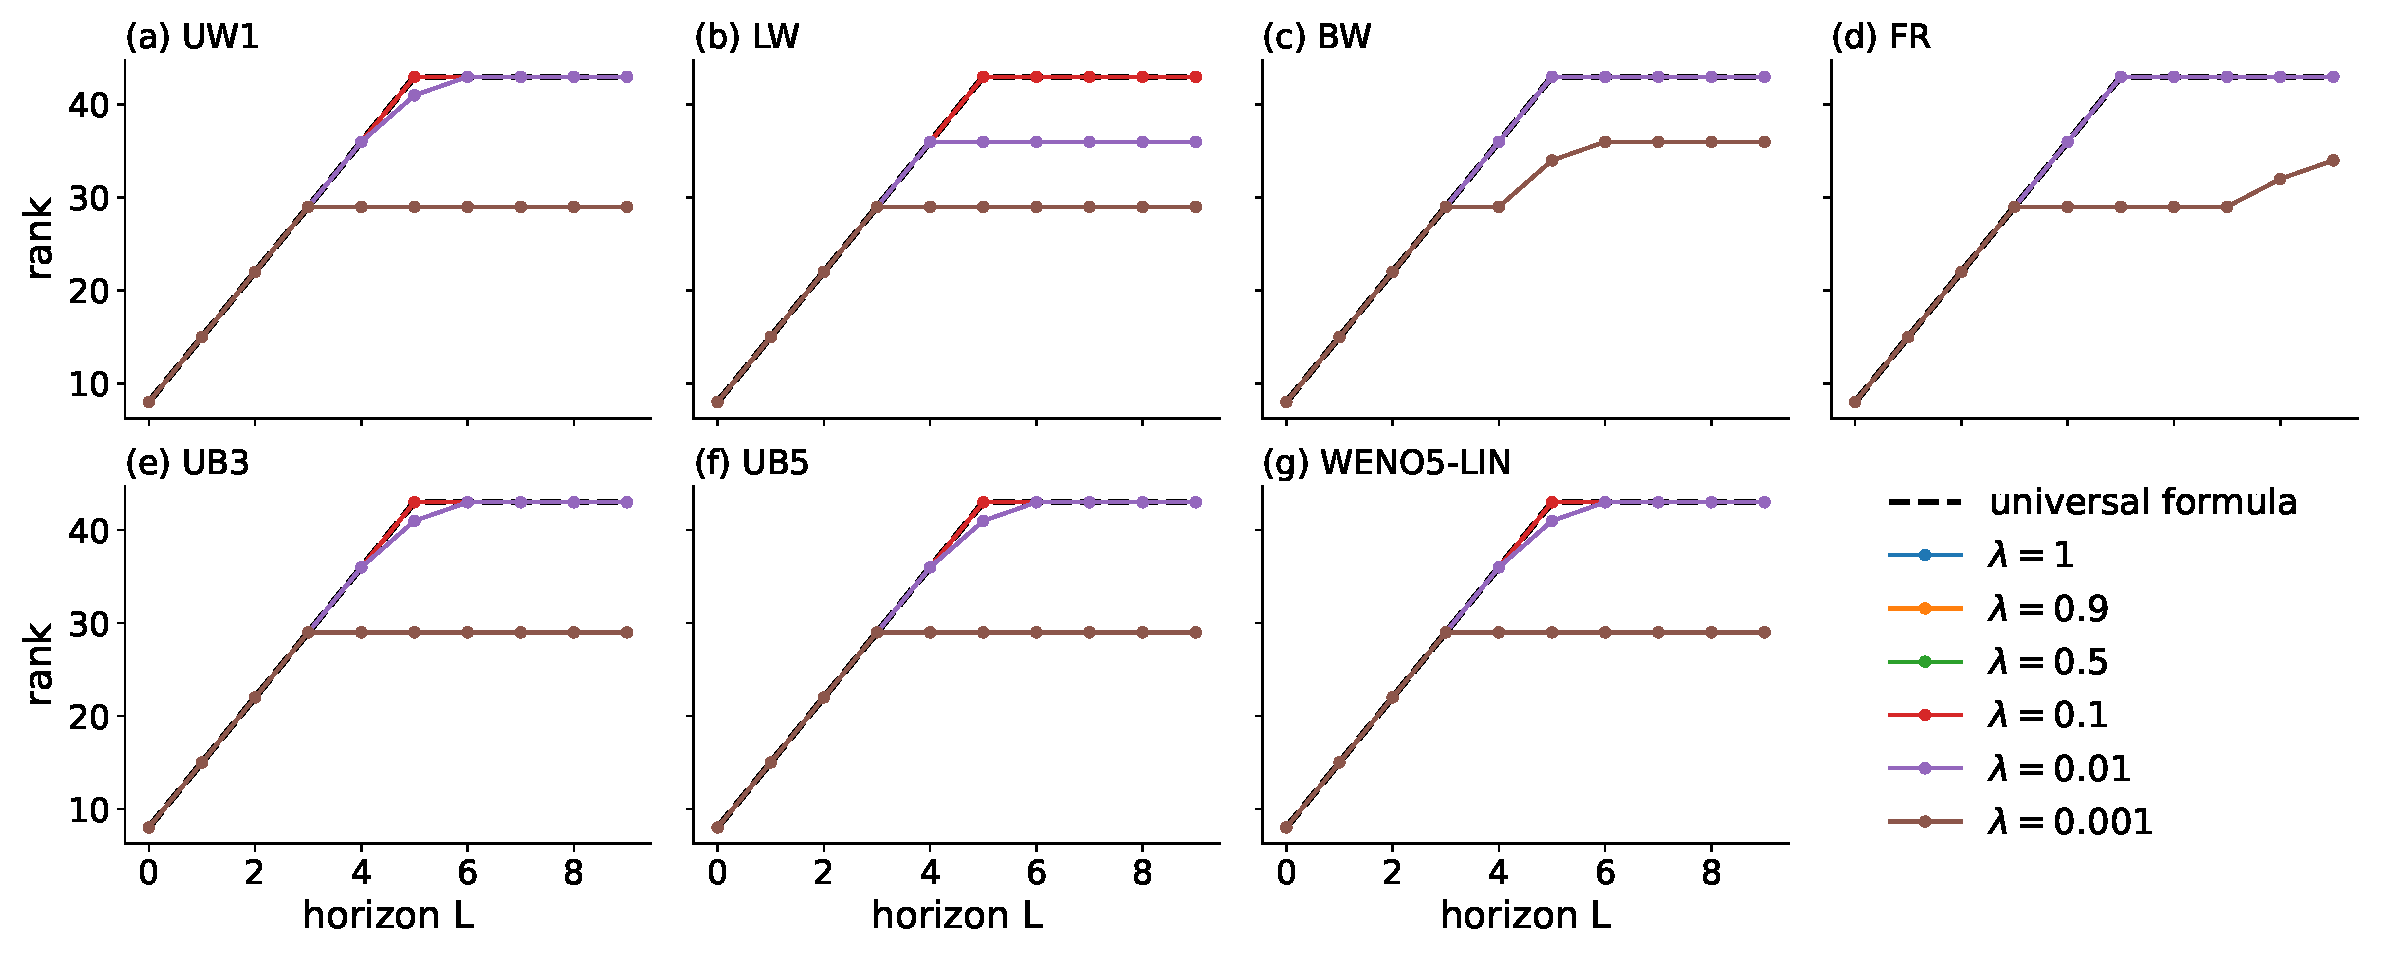
\includegraphics[width=\textwidth]{figures/rank_ladders_linear.pdf}
\caption{Rank ladders for the linear scheme family: effective (SVD) rank of $\OL$ versus horizon $L$ for $P=8$, $r=6$, one panel per scheme, six Courant numbers, overlaid with the universal formula $P+(P-1)\min\{L,r-1\}$ (black dashed).
For $\lambda\ge0.1$, every curve coincides with the dashed universal ladder for every scheme, confirming \cref{thm:rank-universal}; departures at $\lambda\le0.01$ are effective-rank (conditioning) losses, not violations of the theorem.
Panels (left to right, top to bottom): \textbf{(a)}~UW1, first-order upwind; \textbf{(b)}~LW, Lax--Wendroff; \textbf{(c)}~BW, Beam--Warming; \textbf{(d)}~FR, Fromm; \textbf{(e)}~UB3, upwind-biased $p=3$; \textbf{(f)}~UB5, upwind-biased $p=5$; \textbf{(g)}~WENO5-LIN, linear-weights WENO5 ($+$FE).}
\label{fig:rank-ladders}
\end{figure}

\subsection{E2: saturated spectra and effective rank}\label{sec:exp-spectra}

\Cref{tab:eff-rank-sat} reports the effective rank of the saturated observation matrix ${\cal O}_{r-1}$ ($P=8$, $r=6$, exact rank $43$) throughout the Courant sweep, and \cref{fig:singular-spectra} the corresponding singular spectra.
Every scheme holds the exact rank down to $\lambda=0.05$.
The losses at $\lambda\le0.01$ order the family: Beam--Warming and Fromm are the most robust ($43$ at $\lambda=0.01$), first-order upwind and the upwind-biased/WENO operators lose two directions ($41$), and Lax--Wendroff loses seven ($36$); at $\lambda=10^{-3}$ depth conditioning dominates, and every scheme loses heavily.

\begin{table}[htbp]
\centering
\caption{E2: effective rank $\rank_\tau({\cal O}_{r-1})$ at saturation ($P=8$, $r=6$, exact rank $43$) across the Courant sweep.}
\label{tab:eff-rank-sat}
\begin{tabular}{@{}lccccccc@{}}
\toprule
Scheme    & $\lambda=1$ & $0.9$ & $0.5$ & $0.1$ & $0.05$ & $0.01$ & $0.001$ \\
\midrule
UW1       & 43          & 43    & 43    & 43    & 43     & 41     & 29      \\
LW        & 43          & 43    & 43    & 43    & 43     & 36     & 29      \\
BW        & 43          & 43    & 43    & 43    & 43     & 43     & 34      \\
FR        & 43          & 43    & 43    & 43    & 43     & 43     & 29      \\
UB3       & 43          & 43    & 43    & 43    & 43     & 41     & 29      \\
UB5       & 43          & 43    & 43    & 43    & 43     & 41     & 29      \\
WENO5-LIN & 43          & 43    & 43    & 43    & 43     & 41     & 29      \\
\bottomrule
\end{tabular}
\end{table}

Because the Fourier block-diagonalization in the proof of \cref{thm:rank-universal} is unitary, the spectrum of $\OL$ is the union of the spectra of the class blocks $V_m$, and effective-rank loss can be attributed to individual residue classes.
At $\lambda=0.01$ the worst class block has $\sigma_{\min}(V_m)=2.3\times10^{-11}$ for BW, $5.8\times10^{-13}$ for UW1, and $4.3\times10^{-15}$ for LW (class $m=4$) --- four orders of magnitude apart at identical exact rank.

The mechanism is the first-order node geometry.
Writing $g_k=1+\lambda\mu_k+O(\lambda^2)$ with $\mu_k=\sum_sc_s'(0)\,e^{-i\theta_ks}$ (computed exactly from the coefficient polynomials), the intra-class node gaps are $\lambda\,|\mu_j-\mu_{j'}|$ to leading order.
For UW1, $\mu(\theta)=e^{-i\theta}-1$ is injective on $[0,2\pi)$.
For BW, $\mu(\theta)=2e^{-i\theta}-\tfrac12e^{-2i\theta}-\tfrac32$ is injective (the pair equation $e^{-i\theta}+e^{-i\theta'}=4$ has no solution) with the largest velocity spread in the family --- hence its robustness.
For LW, $\mu(\theta)=-i\sin\theta$ is \emph{purely imaginary}: the node velocities collapse onto a line and coincide exactly for $\theta$ and $\pi-\theta$.
At $(P,r)=(8,6)$ the reflected pairs $(k,k')=(4,20)$ and $(28,44)$ both fall into the class $m=4$, so two node gaps are second order, $|g_4-g_{20}|=\sqrt3\,\lambda^2$ (measured $1.73\times10^{-4}$ at $\lambda=0.01$, against $\Theta(\lambda)$ gaps for every other scheme).
This resolves the E1 observation: Lax--Wendroff's early effective-rank loss is a \emph{node-degeneracy} effect, invisible to exact rank and distinct from the depth-conditioning mechanism of \cref{sec:exp-conditioning}.
Fromm, whose velocity field inherits the real part of BW ($\mu_{\rm FR}=\tfrac12(\mu_{\rm LW}+\mu_{\rm BW})$), remains first-order separated and tracks BW's robustness at $\lambda=0.01$.

\begin{figure}[htbp]
\centering
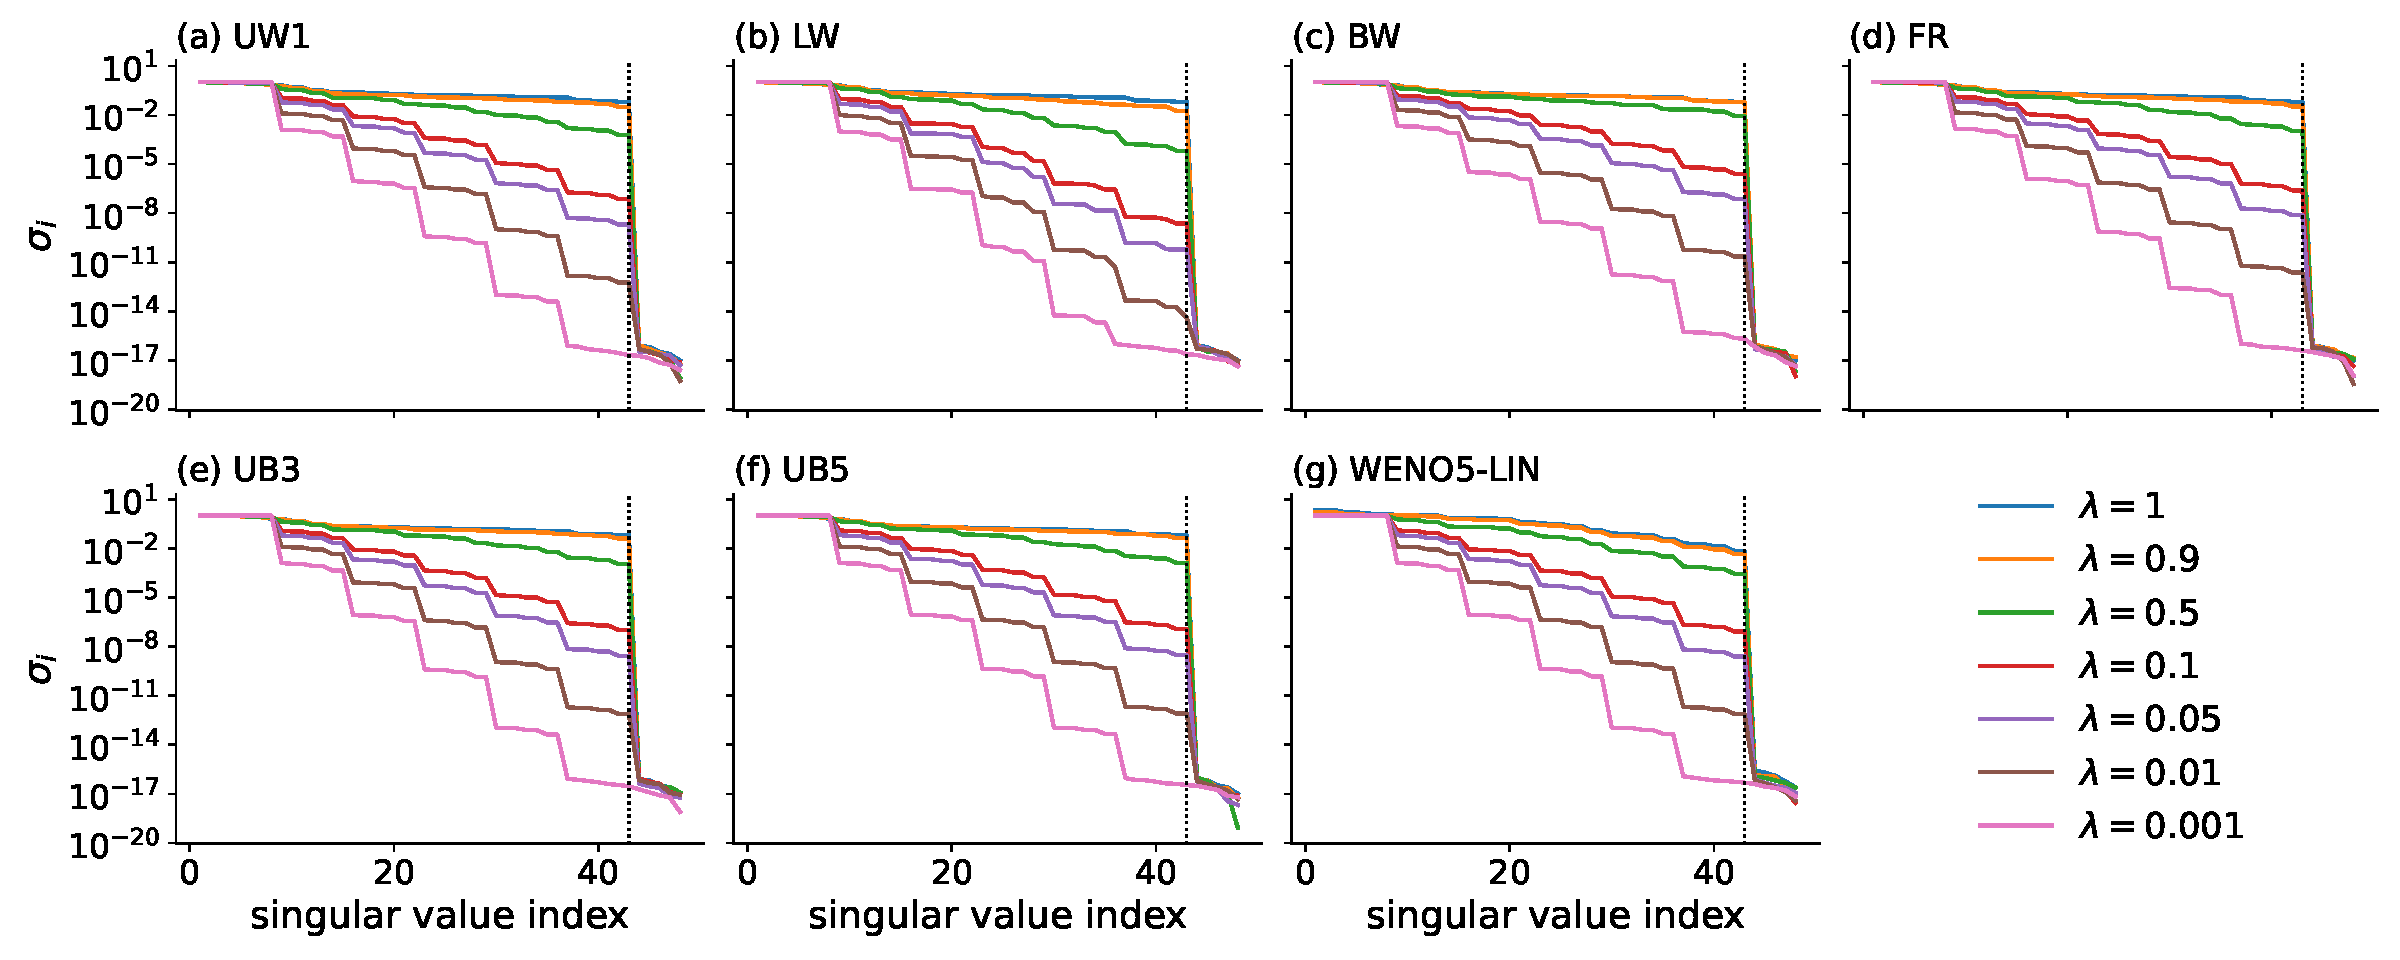
\includegraphics[width=\textwidth]{figures/singular_spectra_saturated.pdf}
\caption{Singular spectra of the saturated observation matrix ${\cal O}_{r-1}$ ($P=8$, $r=6$), one panel per scheme, seven Courant numbers.
The dotted vertical line marks the exact rank $43$.
Spectra to the right of steep drops fall below the declared tolerance and are lost to effective rank; Lax--Wendroff's class-$m{=}4$ node degeneracy is visible as the early plateau collapse at $\lambda=0.01$.
Panels (left to right, top to bottom): \textbf{(a)}~UW1, first-order upwind; \textbf{(b)}~LW, Lax--Wendroff; \textbf{(c)}~BW, Beam--Warming; \textbf{(d)}~FR, Fromm; \textbf{(e)}~UB3, upwind-biased $p=3$; \textbf{(f)}~UB5, upwind-biased $p=5$; \textbf{(g)}~WENO5-LIN, linear-weights WENO5 ($+$FE).}
\label{fig:singular-spectra}
\end{figure}

\subsection{E3: queue conditioning}\label{sec:exp-conditioning}

E3 measures the object of \cref{conj:conditioning} directly: the smallest nonzero singular value $\sigma^{+}_{\min}$ of the single-parent observation map $\OL\,\iota_K$, which is defined at every horizon.
Within the single-parent window $Lw\le r-1$, \cref{lem:queue-equivalence} identifies it with the generalized queue map $T^{[\rm sch]}_q$ up to $\lambda$-independent constants; at the wraparound horizons beyond that window --- which the sweep enters for every scheme except first-order upwind ($w=1$) --- the observation-map form is the one being tested.
E3 sweeps $\lambda\in[10^{-3},0.5]$ (15 logarithmically spaced values) and horizons $L=1,\ldots,r-1$, and fits the exponent $\gamma=\mathrm d\log\sigma^{+}_{\min}/\mathrm d\log\lambda$ on $\lambda\le0.05$.
The singular values are computed in the coordinates of the basis $e_j-e_0$ ($j=1,\ldots,r-1$) of the zero-mean subspace rather than in its induced Euclidean norm; this basis is not orthonormal, but its Gram matrix has eigenvalues $1$ and $r$, so every singular value changes by a $\lambda$-independent factor in $[1,\sqrt r]$ and the fitted exponents are unaffected.
\Cref{tab:queue-exponents} compares the fits with the prediction $\gamma=L_q$ of \cref{conj:conditioning}: the largest deviation across all $35$ scheme--horizon pairs is $0.05$.
The measurements are consistent with the conjectured law in both regimes; they support the conjecture but do not prove it.

\begin{table}[htbp]
\centering
\caption{E3: fitted conditioning exponents $\gamma_{\rm sch}$ (predicted $L_q$ in parentheses), from log--log slopes of $\sigma^{+}_{\min}(\OL\iota_K)$ over $\lambda\le0.05$, at $P=8$, $r=6$.}
\label{tab:queue-exponents}
\begin{tabular}{@{}lccccc@{}}
\toprule
Scheme    & $L=1$    & $L=2$    & $L=3$    & $L=4$    & $L=5$    \\
\midrule
UW1       & 1.00 (1) & 2.00 (2) & 3.01 (3) & 4.01 (4) & 5.02 (5) \\
LW        & 1.01 (1) & 1.99 (2) & 3.00 (3) & 3.00 (3) & 3.00 (3) \\
BW        & 1.00 (1) & 2.00 (2) & 3.00 (3) & 3.95 (4) & 3.95 (4) \\
FR        & 0.99 (1) & 1.99 (2) & 3.00 (3) & 3.00 (3) & 2.99 (3) \\
UB3       & 0.99 (1) & 1.98 (2) & 3.02 (3) & 3.01 (3) & 3.01 (3) \\
UB5       & 1.00 (1) & 1.98 (2) & 3.01 (3) & 3.01 (3) & 3.01 (3) \\
WENO5-LIN & 1.00 (1) & 2.00 (2) & 3.00 (3) & 3.00 (3) & 3.00 (3) \\
\bottomrule
\end{tabular}
\end{table}

Three rows carry the message.
First-order upwind reproduces the triangular law $\gamma=q$ of \cite{PolemitisChristakisDrikakis2026FVerasure} exactly ($1,\ldots,5$).
Every two-collar scheme saturates at $\gamma=3=\lceil(r-1)/2\rceil$: at the saturated memory dimension $q=5$, recovering the deepest direction costs $\lambda^{3}$ instead of UW1's $\lambda^{5}$ --- at $\lambda=0.01$, four orders of magnitude of tolerance headroom, the conditioning dividend of the second collar.
Beam--Warming, though one-sided, gains one exponent through its wrap-around exposure ($\gamma=4$ at $L\ge4$, where its support first spans a second downstream parent).
Notably, the exponents are identical for LW and the wide two-sided stencils (FR, UB3, UB5, WENO5-LIN): for these single-stage operators, depth conditioning counts only collars and exposure times, in exact analogy with the local rank law of \cref{prop:local-rank}.

\begin{figure}[htbp]
\centering
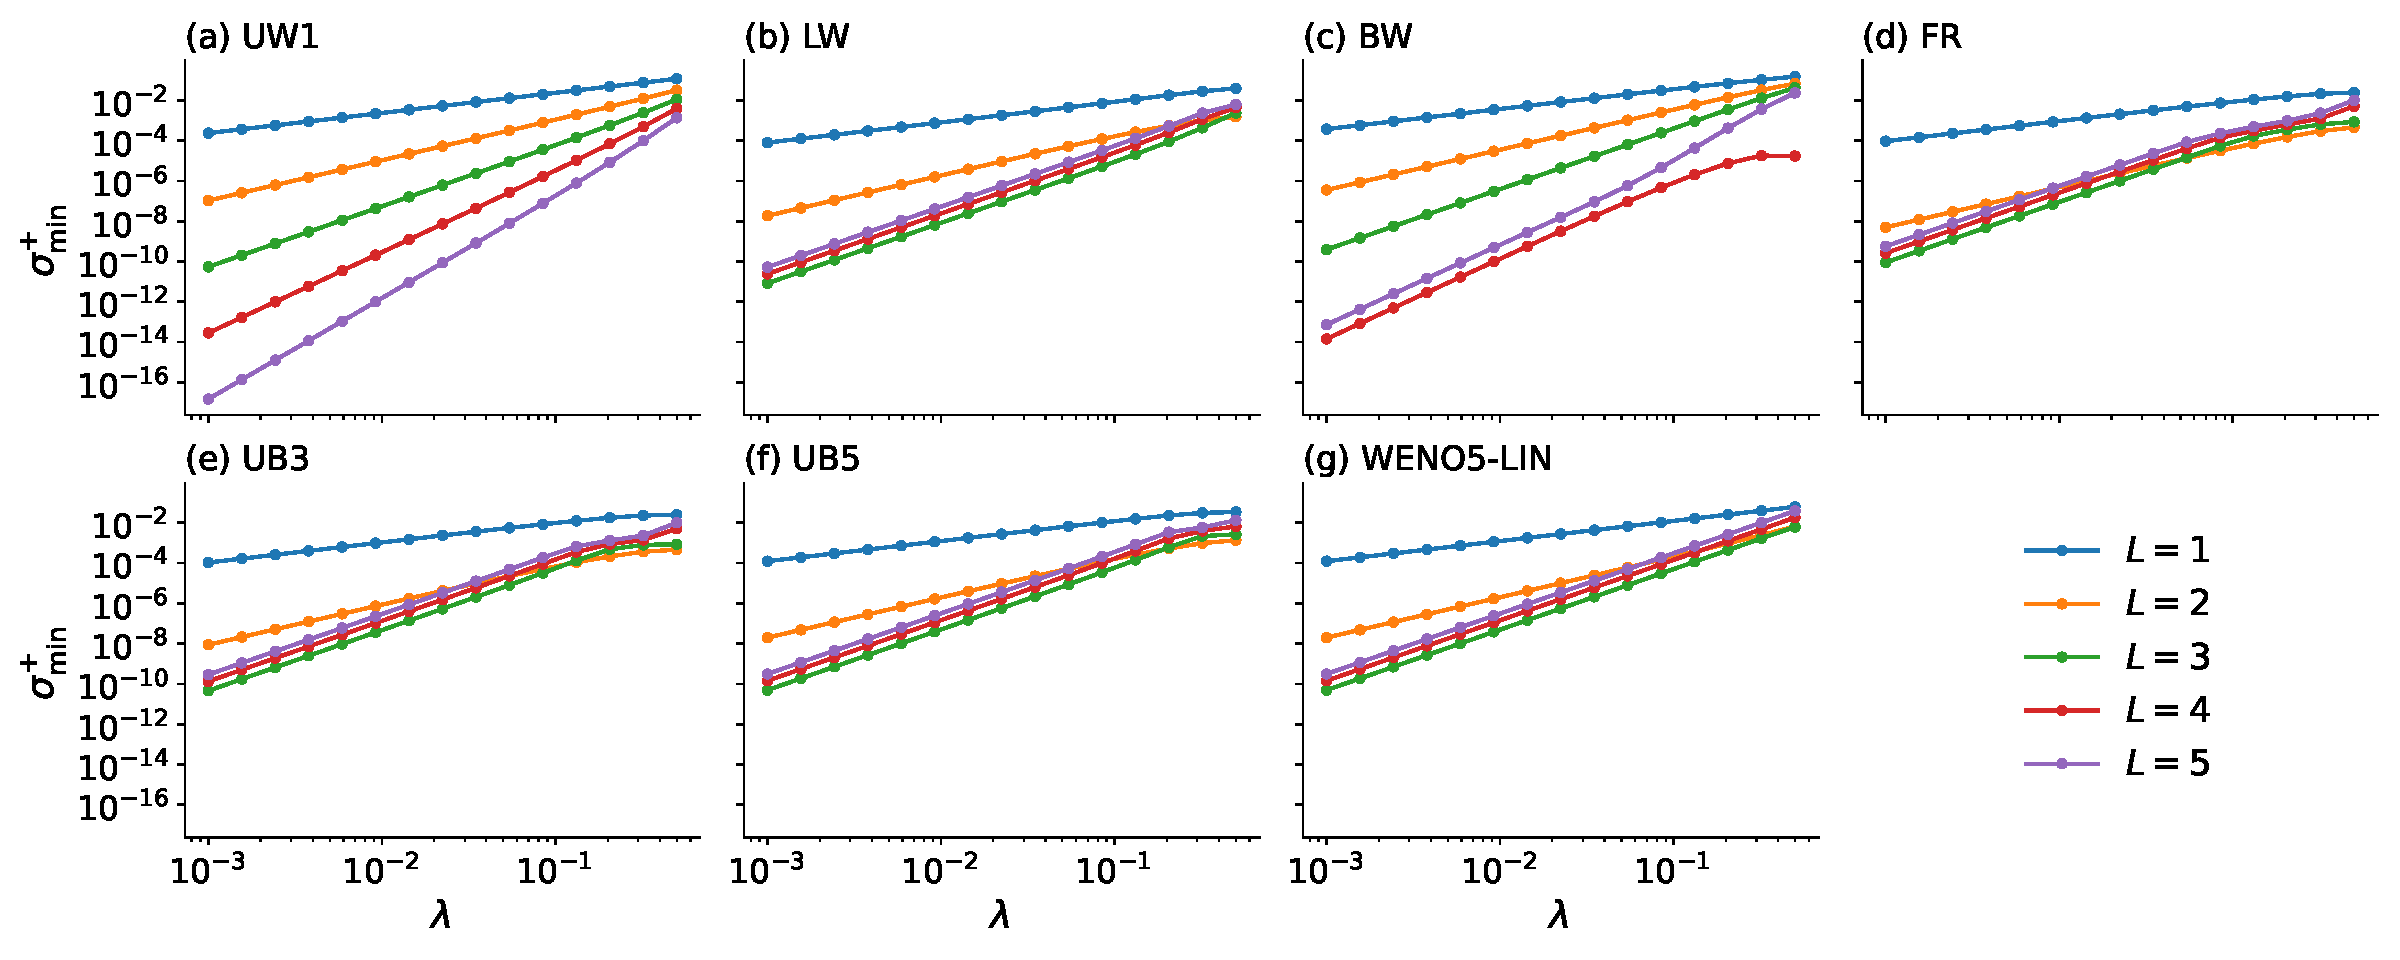
\includegraphics[width=\textwidth]{figures/queue_conditioning.pdf}
\caption{E3: smallest nonzero singular value of the single-parent observation map versus Courant number (log--log), one panel per scheme, horizons $L=1,\ldots,5$.
Slopes match the predicted exponents $\gamma=L_q$ of \cref{conj:conditioning} (\cref{tab:queue-exponents}).
Panels (left to right, top to bottom): \textbf{(a)}~UW1, first-order upwind; \textbf{(b)}~LW, Lax--Wendroff; \textbf{(c)}~BW, Beam--Warming; \textbf{(d)}~FR, Fromm; \textbf{(e)}~UB3, upwind-biased $p=3$; \textbf{(f)}~UB5, upwind-biased $p=5$; \textbf{(g)}~WENO5-LIN, linear-weights WENO5 ($+$FE).}
\label{fig:queue-conditioning}
\end{figure}

\subsection{E4: erasure rates and step flattening}\label{sec:exp-erasure}

E4 validates \cref{prop:dissipation,prop:weno-fe,prop:contraction-general} in four parts.
\emph{(a) Exact orders.}
The moment polynomials of \cref{lem:amplitude} are computed in rational arithmetic for all eight fully discrete operators; the orders and leading coefficients are exactly those of \cref{prop:dissipation,prop:weno-fe} (the low moments vanish identically), and the interior-stability factorizations of \cref{prop:interior-stability} are certified as exact polynomial identities.
\emph{(b) Stability scan and exact certificate.}
$\max_k|g(\theta_k)|$ on a dense frequency grid ($N=2048$) over $\lambda=0.05,\ldots,1$ corroborates \cref{prop:interior-stability}: the scan finds exactly one violator, WENO5-LIN + FE, at every $\lambda$; at the nondissipative endpoint $\lambda=1$ every semi-Lagrangian member returns $\max_k|g_k|=1$ to machine zero (pure shift), while WENO5-LIN + SSP-RK3 remains strictly dissipative.
For this pairing, the scan is superseded by \emph{E4e}, the exact two-region Bernstein certificate of \cref{prop:rk3-stability} (decomposition verified exactly; $S\ge0.1440$ on $[-1,1]\times[0,\tfrac12]$ and $Q/\lambda\ge\tfrac1{24}$ on $[-1,1]\times[\tfrac12,1]$, one Bernstein cell each), for which the grid scan is now merely an independent cross-check.
\emph{(c) The $N^{-2s}$ law.}
\Cref{fig:erasure-rates} reports $|1-\rho_N|$ for $N\in\{24,48,96,192,384\}$ at $\lambda\in\{0.5,0.9\}$.
Log--log slopes fitted on the last three $N$ match $-2s$ to three decimals for every stable scheme ($-2.000$, $-4.000$, $-6.000$, and $-5.999$ for UB5 at $\lambda=0.9$; WENO5-LIN + SSP-RK3 $-4.009$ and $-4.001$), and the ratio $(1-\rho_N)/[\tfrac12A(\lambda)\theta_1^{2s}]$ at $N=384$ lies in $[0.9999,1.0009]$ for all schemes and both $\lambda$.
For UB5 at $\lambda=0.9$ these two values are evaluated in high-precision arithmetic ($0.99994$ and $-5.9994$): there $1-\rho_{384}\approx3\times10^{-14}$, which double precision does not resolve, and the double-precision entries of \texttt{erasure\_rate\_fits.csv} ($0.989$ and $-6.007$) carry that rounding error.
WENO5-LIN + FE shows the predicted pathology: $\rho_N-1\approx+0.19$ at $\lambda=\tfrac12$, flat in $N$ (interior-frequency maximum).
\emph{(d) Step flattening.}
A step function at $N=64$, $\lambda=\tfrac12$ is evolved for $2\times10^5$ steps (\cref{fig:erasure-flattening}): first-order upwind flattens to below $10^{-17}$ within $\sim3\times10^4$ steps, while at the end of the run the four $2s=4$ semi-Lagrangian members still retain $58\%$ of their nonconstant $L^2$ norm, WENO5-LIN + SSP-RK3 retains $86\%$, and UB5 retains $91\%$.
At this Courant number, the quartet collapses pairwise (\cref{rem:coefficient-structure}(iii)): FR and UB3 are the same operator, so their curves are identical; LW and BW share amplitude spectra, so their norm histories agree to roundoff ($2\times10^{-14}$); and the two pairs stay within $3.5\times10^{-4}$ relative to each other over the whole run (final retentions $0.5831$ and $0.5829$) --- the seven legend entries therefore produce only four distinguishable curves.
The per-step contraction, measured on the slowest mode, reproduces $\rho_N$ to machine precision (largest deviation $2.2\times10^{-16}$ across the family), and the mean drift stays below $6\times10^{-15}$ (exact conservation).
The step-function tail itself is a mode mixture and is pre-asymptotic at this horizon for $2s\ge6$ --- an experimental restatement of how slowly sixth-order dissipation acts.

\begin{figure}[htbp]
\centering
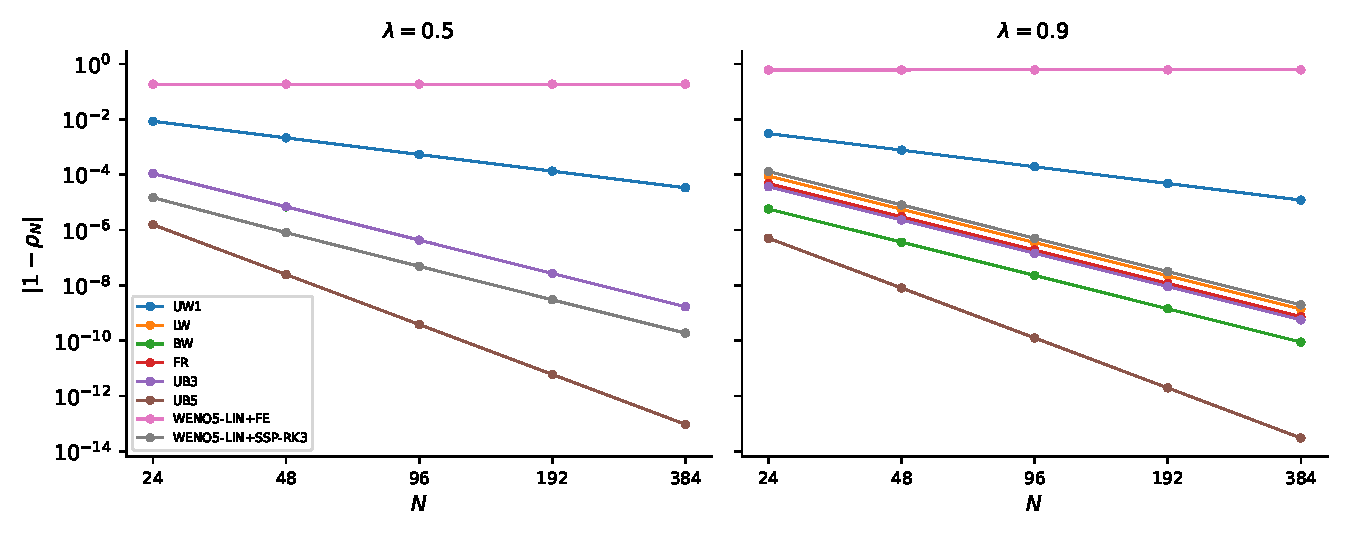
\includegraphics[width=0.85\textwidth]{figures/erasure_rates.pdf}
\caption{E4c: $|1-\rho_N|$ versus $N$ (log--log) at $\lambda=0.5$ (left) and $0.9$ (right).
Slopes match the dissipative orders $-2s$ of \cref{prop:dissipation} to three decimals; the flat top curve is the WENO5-LIN + FE instability ($\rho_N>1$, $N$-independent).
At $\lambda=0.5$ the four $2s=4$ semi-Lagrangian members overlay: LW/BW and FR/UB3 coincide pairwise exactly at this $\lambda$, and the two pairs share the leading coefficient $A=\tfrac3{64}$ (\cref{rem:coefficient-structure}(iii)).}
\label{fig:erasure-rates}
\end{figure}

\begin{figure}[htbp]
\centering
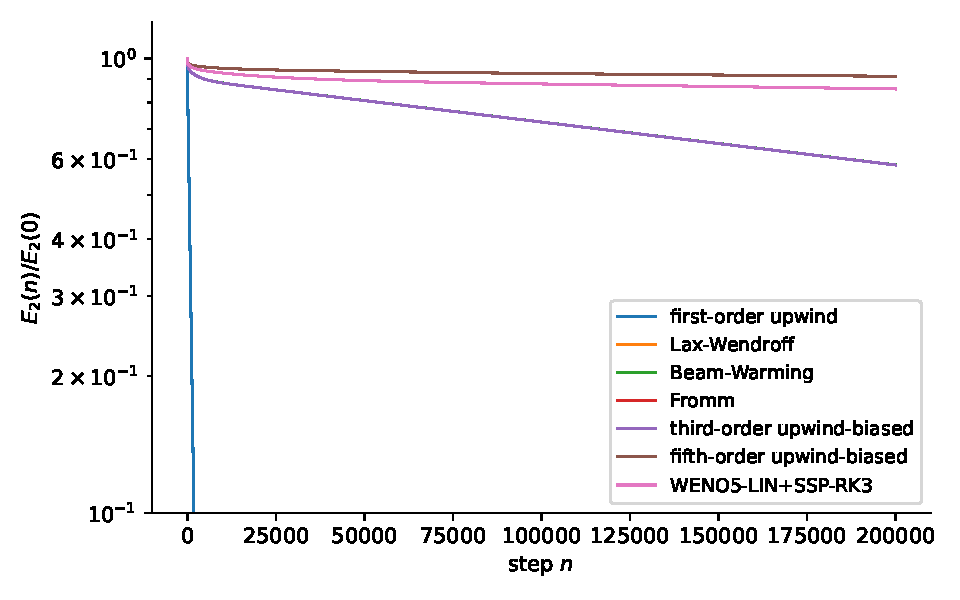
\includegraphics[width=0.7\textwidth]{figures/erasure_flattening.pdf}
\caption{E4d: step-function flattening --- norm retention $E_2(n)/E_2(0)$, with $E_2(n)$ the $\ell^2$ norm of the zero-mean (nonconstant) part of the state after $n$ steps --- over $2\times10^5$ steps ($N=64$, $\lambda=0.5$).
The vertical axis is clipped at $10^{-1}$ so that the high-order members can be compared; first-order upwind exits the frame by step $n\approx2\times10^3$ and continues geometrically---a straight line on the logarithmic axis with per-step factor $\rho_N=0.99880$---reaching $10^{-17}$ by $n\approx3.2\times10^4$, in agreement with the slowest-mode prediction $\ln(10^{17})/(-\ln\rho_N)\approx3.25\times10^4$.
Every high-order member still retains $58\%$--$91\%$ of its nonconstant $L^2$ norm at the end of the run.
Only four of the seven curves are distinguishable: at $\lambda=\tfrac12$ LW/BW and FR/UB3 coincide pairwise --- exactly --- and the two pairs differ by less than the line width (\cref{rem:coefficient-structure}(iii)).}
\label{fig:erasure-flattening}
\end{figure}

\subsection{E5: delayed collisions and the information half-life}\label{sec:exp-collisions}

E5 repeats the delayed-collision experiment of \cite{PolemitisChristakisDrikakis2026FVerasure} across the family ($P=8$, $r=6$, $N=48$, $\lambda=\tfrac12$, detection threshold $\zeta=10^{-12}$).
For each scheme and each admissible depth $t_0\le\lfloor(r-1)/w\rfloor$, the sharp compensated pair of \cref{cor:detection-delay} ($v=e_{j_2}-e_{j_1}$, $j_2=r-t_0m_L$, $j_1=t_0m_R$) evolves for $3\times10^5$ steps and its coarse trace $\|R(\Asch)^nv\|_2$ is recorded (\cref{fig:delayed-collisions}).
Across the $12$ (scheme, depth) pairs with $t_0\ge1$ the first separation occurs \emph{exactly} at the predicted step $t^\ast=t_0$ --- coarse averages are zero to roundoff ($\sim10^{-17}$) through step $t_0-1$ and jump to $O(10^{-1})$ at $t_0$ --- confirming the sharpness of the detection-delay law for the prescribed pairs: geometric shielding of five steps for UW1 ($t_0=1,\ldots,5$), two for LW and BW, and one for FR, UB3, and UB5.
WENO5-LIN + SSP-RK3, whose tripled reach ($w=15>r-1$) admits no shielding at all at this refinement ratio ($t_0=0$), is detected immediately, at the first step, as predicted.

\Cref{tab:half-life} reports the main diagnostic announced in \cref{rem:double-penalty}.
The predicted half-life $n_{1/2}=\ln2/(-\ln\rho_N)$ is confirmed by the fitted tail decay to four significant digits for every scheme whose tail is asymptotic within the horizon; for UB5 and WENO5-LIN + SSP-RK3 the $3\times10^5$-step window is still a mode mixture (adjacent modes decay within a factor $e$ of each other over the whole run), so the fitted values underestimate the true half-life --- the retention entries for these schemes are, if anything, conservative.
The predicted column does not require longer runs in any case: it is $\ln2/(-\ln\rho_N)$ with $\rho_N$ independently verified to machine precision by the slowest-mode contraction fits of E4d (largest deviation $2.2\times10^{-16}$), so the daggered fits play a purely illustrative role.
The two-order-of-magnitude gap between complete local detection ($T_{\rm loc}\le5$ steps) and retention ($3\times10^2$ to $3\times10^7$ steps) is the quantitative content of the revised penalty (\cref{rem:double-penalty}).

\begin{table}[htbp]
\centering
\caption{E5: geometric shielding time, local injectivity horizon, and information half-life at $N=48$, $\lambda=\tfrac12$.
Shielding $\le$ is the deepest admissible $t_0$ of the \emph{prescribed} compensated pair (measured $=$ predicted in every case) --- a best case for the scheme, not the worst-case delay, which is $r-1$ for every scheme (\cref{cor:detection-delay}(i)).
$T_{\rm loc}=\min\{L:\rho(L)=r-1\}$ is the horizon by which every localized zero-mean perturbation is detectable (E1c).
$n_{1/2}=\ln2/(-\ln\rho_N)$, exact for geometric decay; the fitted value is the tail-decay estimate ($^\dagger$pre-asymptotic window, underestimates retention).
LW and BW share $\rho_N$ exactly at $\lambda=\tfrac12$, and FR and UB3 are the same operator there, so each pair's entries agree (\cref{rem:coefficient-structure}(ii)--(iii)).}
\label{tab:half-life}
\begin{tabular}{@{}lccccc@{}}
\toprule
Scheme            & shielding $\le$ & $T_{\rm loc}$ & $n_{1/2}$ (pred.) & $n_{1/2}$ (fit)               & retention vs.\ UW1 \\
\midrule
UW1               & 5               & 5             & $3.234\times10^2$ & $3.234\times10^2$             & $1$                \\
LW                & 2               & 3             & $1.010\times10^5$ & $1.010\times10^5$             & $312$              \\
BW                & 2               & 4             & $1.010\times10^5$ & $1.010\times10^5$             & $312$              \\
FR                & 1               & 3             & $1.009\times10^5$ & $1.009\times10^5$             & $312$              \\
UB3               & 1               & 3             & $1.009\times10^5$ & $1.009\times10^5$             & $312$              \\
UB5               & 1               & 3             & $2.829\times10^7$ & $6.830\times10^5$\,$^\dagger$ & $87{,}490$         \\
WENO5-LIN+SSP-RK3 & 0               & 2             & $8.608\times10^5$ & $7.507\times10^5$\,$^\dagger$ & $2{,}662$          \\
\bottomrule
\end{tabular}
\end{table}

\begin{figure}[htbp]
\centering
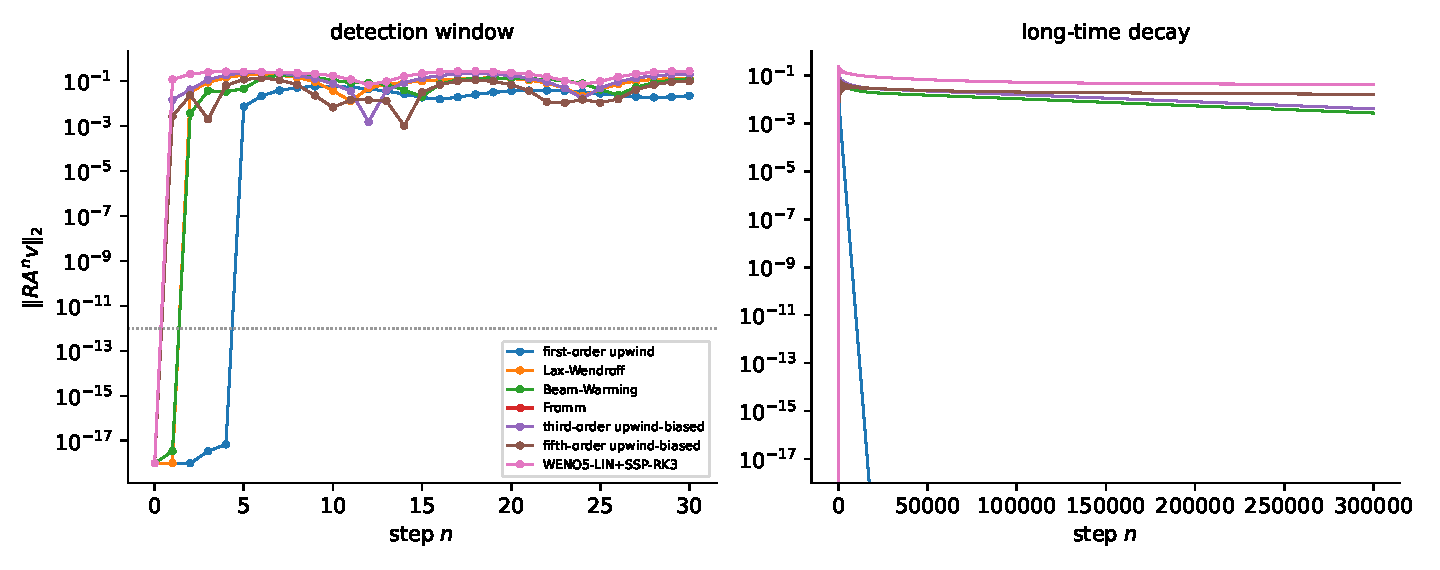
\includegraphics[width=\textwidth]{figures/delayed_collisions.pdf}
\caption{E5: coarse separation $\|R(\Asch)^nv\|_2$ of the deepest sharp pair per scheme.
Left: detection window --- each curve sits at the roundoff floor ($\sim10^{-17}$) through step $t_0-1$ and crosses the threshold (dotted) exactly at the predicted step, $t_0=5$ for UW1 down to $t_0\le1$ for the widest stencils.
Right: long-time decay over $3\times10^5$ steps --- the detection ordering reverses; first-order upwind erases its trace almost immediately on this axis while the high-order schemes retain theirs for $10^5$--$10^7$ steps (\cref{tab:half-life}).}
\label{fig:delayed-collisions}
\end{figure}

\subsection{E6: nonlinear ensembles}\label{sec:exp-nonlinear}

E6 runs the protocol of \cref{sec:collision-protocol} for the seven nonlinear schemes of \cref{sec:nonlinear-family}.
\Cref{tab:nonlinear} reports, at the quasi-linear amplitude $\varepsilon=10^{-5}$, the deep-pair detection step, the empirical response-span and linearized rank ladders, and the nonlinearity gap at both amplitudes; \cref{fig:nonlinear-ladders} plots the ladders against the linear reference laws.
Four findings organize the data.

\begin{table}[htbp]
\centering
\caption{E6 summary at $(P,r)=(8,6)$, $\lambda=\tfrac12$, $M=400$ random members plus the deep pair.
Ladders $\rho(1),\dots,\rho(5)$ and the horizon-$12$ empirical response-span rank at amplitude $\varepsilon=10^{-5}$ and leading floor $\theta=10^{-3}$; the nonlinearity gap $\sigma_6/\sigma_1$ of $D_5$ at both amplitudes.
In the jump regime, the gap at $L=5$ sits at the roundoff floor for the MUSCL schemes because the response staircase reaches six directions only at $L=6$.}
\label{tab:nonlinear}
\begin{tabular}{@{}lcllcll@{}}
\toprule
Scheme                                   & $t_\star^{\rm deep}$        & $\rho^{\rm emp}_\theta(1..5)$ &
$\rho^{\rm lin}(1..5)$                   & $\rho^{\rm emp}_\theta(12)$ &
$\tfrac{\sigma_6}{\sigma_1}$ ($10^{-5}$) &
$\tfrac{\sigma_6}{\sigma_1}$ ($10^{-2}$)                                                                                                                           \\
\midrule
\multicolumn{7}{@{}l}{\emph{smooth (monotone parent)}}\\
MUSCL minmod                             & 4                           & 1,2,3,4,5                     & 1,2,3,4,5 & 7  & $4.4\times10^{-11}$ & $7.6\times10^{-3}$ \\
MUSCL MC                                 & 2                           & 2,4,5,5,5                     & 2,4,5,5,5 & 5  & $2.6\times10^{-11}$ & $<\!10^{-13}$      \\
MUSCL van Leer                           & 2                           & 2,4,5,5,5                     & 2,4,5,5,5 & 5  & $1.5\times10^{-6}$  & $1.5\times10^{-3}$ \\
MUSCL superbee                           & 2                           & 2,4,5,6,6                     & 2,4,5,5,5 & 7  & $4.2\times10^{-3}$  & $1.5\times10^{-2}$ \\
WENO5-JS                                 & 1                           & 2,4,5,5,5                     & 3,5,5,5,5 & 5  & $8.9\times10^{-6}$  & $5.8\times10^{-3}$ \\
WENO5-M                                  & 1                           & 2,4,5,5,5                     & 3,5,5,5,5 & 5  & $6.2\times10^{-9}$  & $2.3\times10^{-3}$ \\
WENO5-Z                                  & 1                           & 2,4,5,5,5                     & 3,5,5,5,5 & 5  & $1.0\times10^{-6}$  & $1.8\times10^{-3}$ \\
\midrule
\multicolumn{7}{@{}l}{\emph{extremum (peak-centered parent)}}\\
MUSCL minmod                             & 2                           & 2,4,5,6,7                     & 2,4,5,5,5 & 7  & $5.8\times10^{-3}$  & $1.1\times10^{-2}$ \\
MUSCL MC                                 & 2                           & 2,4,5,6,7                     & 2,4,5,5,5 & 8  & $4.8\times10^{-3}$  & $1.1\times10^{-2}$ \\
MUSCL van Leer                           & 2                           & 2,4,5,6,7                     & 2,4,5,5,5 & 8  & $4.2\times10^{-3}$  & $6.2\times10^{-3}$ \\
MUSCL superbee                           & 3                           & 1,2,3,4,5                     & 1,2,3,4,5 & 7  & $4.0\times10^{-11}$ & $1.3\times10^{-2}$ \\
WENO5-JS                                 & 1                           & 2,4,5,5,5                     & 3,5,5,5,5 & 5  & $2.7\times10^{-5}$  & $1.5\times10^{-2}$ \\
WENO5-M                                  & 1                           & 2,4,5,5,5                     & 3,5,5,5,5 & 5  & $3.4\times10^{-8}$  & $1.3\times10^{-2}$ \\
WENO5-Z                                  & 1                           & 2,4,5,5,5                     & 3,5,5,5,5 & 5  & $5.9\times10^{-7}$  & $9.3\times10^{-3}$ \\
\midrule
\multicolumn{7}{@{}l}{\emph{jump (flat plateau upstream of the discontinuity)}}\\
MUSCL minmod                             & 3                           & 1,2,3,4,5                     & 1,2,3,4,5 & 12 & $4.4\times10^{-11}$ & $<\!10^{-13}$      \\
MUSCL MC                                 & 3                           & 1,2,3,4,5                     & 1,2,3,4,5 & 12 & $4.0\times10^{-11}$ & $<\!10^{-13}$      \\
MUSCL van Leer                           & 3                           & 1,2,3,4,5                     & 1,2,3,4,5 & 11 & $4.4\times10^{-11}$ & $<\!10^{-13}$      \\
MUSCL superbee                           & 3                           & 1,2,3,4,5                     & 1,2,3,4,5 & 13 & $3.9\times10^{-11}$ & $<\!10^{-13}$      \\
WENO5-JS                                 & 1                           & 2,4,5,5,5                     & 2,5,5,5,5 & 5  & $6.0\times10^{-6}$  & $5.6\times10^{-3}$ \\
WENO5-M                                  & 1                           & 2,4,5,5,5                     & 2,5,5,5,5 & 5  & $1.7\times10^{-6}$  & $8.4\times10^{-3}$ \\
WENO5-Z                                  & 1                           & 1,2,3,4,5                     & 1,2,3,5,5 & 12 & $3.5\times10^{-5}$  & $2.8\times10^{-5}$ \\
\bottomrule
\end{tabular}
\end{table}

\paragraph{The active limiter branch, not the nominal stencil, sets the local exposure rate.}
At $\varepsilon=10^{-5}$ the response-span ladders match the linearized ones through saturation in almost every entry, so the local laws of \cref{sec:local} apply to the linearization --- but with an \emph{effective} collar count read off the limiter's active branch, exactly as \cref{prop:active-branch} prescribes: the branch $\varphi=1$ is LW (both collars active), the branch $\varphi(r)=r$ is BW (upstream collar dead), the clipped branch $\varphi=0$ is UW1, and MC's central branch is the Fromm blend.
Minmod takes the BW branch where slopes accelerate ($r<1$) and superbee takes it where they decelerate ($1<r<2$); consequently minmod climbs at $\sigma=1$ on the smooth monotone parent (ladder $1,2,3,4,5$; deep pair detected at step $4$, the one-sided bound) while MC, van Leer, and superbee climb at $\sigma=2$ (ladder $2,4,5$; deep pair at the two-collar bound $t_\star=2$), and the roles reverse at the extremum, where superbee drops to $\sigma=1$ and minmod retains $\sigma=2$.
MC and van Leer keep both collars active in both smooth regimes --- MC through its Fromm-blend central branch, van Leer through its tangent-line blend (\cref{rem:tangent-blend}, upstream weight $2\rho^2/(1+\rho)^2>0$).
The measured deep-pair times all fall in the predicted bracket $[2,4]$ of \cref{sec:collision-protocol}, and the WENO schemes detect at $t_\star=1$ as forced by their $15$-cell reach.

\paragraph{Plateau degeneracy and the nonlinear staircase.}
On the flat plateau, every limiter clips (exactly flat pairs: $r_i$ is $0/0$, and the limited term vanishes by the convention of \cref{sec:nonlinear-family}), so the linearization of every MUSCL scheme is exactly UW1: all four linearized ladders are $1,2,3,4,5$ --- the $\sigma=1$ law.
However, the empirical response-span ladders do \emph{not} saturate at $r-1=5$: they continue at one dimension per step up to $\rho^{\rm emp}_\theta(12) \approx 12$, and are identical at $\varepsilon=10^{-2}$ and $10^{-5}$, confirming that the plateau update is positively homogeneous of degree one.
The scale-free nonlinearity is thus a genuine distinguishability channel: at each step, the sign pattern of the evolving perturbation reconfigures the limiter branches and produces one further independent \emph{response} direction that no linear scheme could produce, so the span of coarse responses grows past the Jacobian image and past the linear budget of \cref{prop:local-rank}.
The staircase is a response-span statement, not extra state: the perturbation space still has $r-1=5$ dimensions, and no additional state coordinates are being observed --- what grows is the richness of the map from those five coordinates to coarse histories.

\paragraph{The regularization scale \texorpdfstring{$\epsilon_w$}{epsilon\_w} decides when WENO is effectively linear.}
With Jiang--Shu regularization $\epsilon_w=10^{-6}$, smoothness indicators of a plateau perturbation scale as $\beta\sim\varepsilon^2$; at $\varepsilon=10^{-5}$ they are dominated by $\epsilon_w$ and the weights sit within $O(\beta/\epsilon_w)=O(\varepsilon^2/\epsilon_w)$ of their linear values: WENO5-JS/M are indistinguishable from the linear-weight circulant at the measured tolerances (ladders $2,4,5$), the residual weight nonlinearity visible only in the gap ($10^{-6}$--$10^{-9}$).
WENO-Z, regularized at $\epsilon_Z=10^{-40}$, does not linearize at any tested amplitude: while $\beta\gg\epsilon_Z$, its weights depend on scale-invariant ratios of the indicators, and its own crossover $\varepsilon\sim\sqrt{\epsilon_Z}\approx10^{-20}$ lies far below the tested range (below that scale, it would also pin to the linear weights).
Therefore, it inherits the MUSCL-like $\sigma=1$ staircase (ladder $1,2,3,4,5$ continuing to $12$) with an $\varepsilon$-independent gap $\approx3\times10^{-5}$.
The choice of regularization constant is therefore not a numerical detail: it sets the amplitude scale below which a WENO scheme is effectively linear and hence the observability regime that subcell perturbations experience.
This is the observability-side face of a known accuracy mechanism --- the dominance of $\epsilon_w$ over the smoothness indicators, and the prescription $\epsilon_w=\Omega(\Delta x^2)$ under which WENO-JS attains its design order by pinning to the linear weights are analyzed in \cite{ArandigaBaezaBeldaMulet2011} --- reappearing here as the amplitude threshold $\varepsilon\sim\sqrt{\epsilon_w}$ that separates the effectively linear from the nonlinear observability regime.
This is what the WENO5 panels of \cref{fig:nonlinear-ladders} show directly.
In the smooth and extremum regimes (panels~(d),(e)) the Jiang--Shu and mapped weights sit below their linearization threshold, while WENO5-Z --- never weight-pinned, as above --- has its residual nonlinear response on these data below the declared floor $\theta=10^{-3}$ (gaps $\approx10^{-6}$--$10^{-7}$, \cref{tab:nonlinear}), so all three variants produce the \emph{identical} leading-floor ladder $2,4,5$, saturating at $r-1=5$ --- the two-collar law of the spatial reconstruction --- and their solid curves lie exactly on top of one another, as do their dashed FD linearizations (which climb $3,5$: the wrap-around ladder of the composed reach-$15$ operator, E1c); the figure draws the coincident curves with nested line widths so the overlap reads as three superimposed lines rather than missing data.
The variants separate only in the jump regime (panel~(f)), where WENO5-Z's scale-free indicators drive the plateau staircase past $5$ while WENO5-JS/M stay linear, and they differ elsewhere only at the much finer machine floor (\texttt{nonlinear\_ensembles.csv}), which is not plotted.
The overlap in panels~(d),(e) is therefore physically meaningful --- at this amplitude, smooth and extremum data expose no difference between the three WENO5 nonlinearities at the declared floor --- not a plotting artifact.

\paragraph{The nonlinearity gap separates smooth from kinked response.}
Where the base state keeps $r_i$ inside a smooth branch, the gap scales linearly in $\varepsilon$ --- van Leer on smooth data gives $\sigma_6/\sigma_1=1.5\times10^{-3}$ vs.\ $1.5\times10^{-6}$, the exact factor $10^3$ of a quadratic response --- and the mapped WENO weights, whose mapping is designed to have high-order tangency at the linear values, suppress the gap by three additional orders of magnitude relative to Jiang--Shu ($8.9\times10^{-6}\to6.2\times10^{-9}$ smooth, $2.7\times10^{-5}\to3.4\times10^{-8}$ at the extremum).
Where the base state sits on a limiter kink the gap is scale-free: superbee on smooth data ($r\approx1$ is a kink of $\varphi$) retains a gap of $4.2\times10^{-3}$ even at $\varepsilon=10^{-5}$, and at the extremum, where the clipping kink at $r=0$ is engaged, minmod, MC, and van Leer show near-$\varepsilon$-independent gaps $\approx5\times10^{-3}$.
(Superbee's extremum gap at $L=5$ is masked by its slower $\sigma=1$ ladder --- only five directions are exposed by then --- but its horizon-$12$ rank of $7$ shows the same kink-driven overshoot.)
The corresponding empirical ladders exceed the linear budget ($\rho^{\rm emp}_\theta(12)=7$--$8$) even at quasi-linear amplitude.

At $\varepsilon=10^{-2}$ every scheme's gap rises to $10^{-3}$--$10^{-2}$ and the machine-floor ranks reach $20$--$26$ (\texttt{nonlinear\_ensembles.csv}): at finite amplitude, the coarse responses span far more output directions than the $r-1=5$ input dimensions --- the quantitative signature of finite-amplitude response richness, not of additional state coordinates.
One further detail connects to \cref{sec:conditioning}: on smooth data the WENO linearized ladder starts at $\rho^{\rm lin}(1)=3$ (the SSP-RK3 wraparound exposes a third direction through the nine-cell downstream reach), but the empirical leading rank sees only $2$ at $L=1$ --- the third direction is real but sits below the $10^{-3}$ floor, a nonlinear instance of the rank--conditioning gap.

\paragraph{Robustness.}
The qualitative branch, crossover, and plateau conclusions of this subsection are robust to the methodological choices behind them: a one-at-a-time sweep of ensemble size ($100$--$800$), random seed, and FD-Jacobian step (E6s, Supplementary Material Sec.~S2) leaves every reported ladder unchanged, single borderline horizon-12 cells aside, and the amplitude axis reproduces the crossover and scale-freeness claims above.
The numerical response-span ranks themselves remain \emph{intentionally} dependent on the declared singular-value floor, particularly at long horizons --- loosening the floor to $10^{-2}$ or tightening it to $10^{-4}$ changes the horizon-12 rank in roughly half of the $21$ cells (by up to seven and four dimensions, respectively; Supplementary Material Sec.~S2) --- because response-span rank is a tolerance-indexed quantity by construction (\cref{def:empirical-rank}).

\begin{figure}[htbp]
\centering
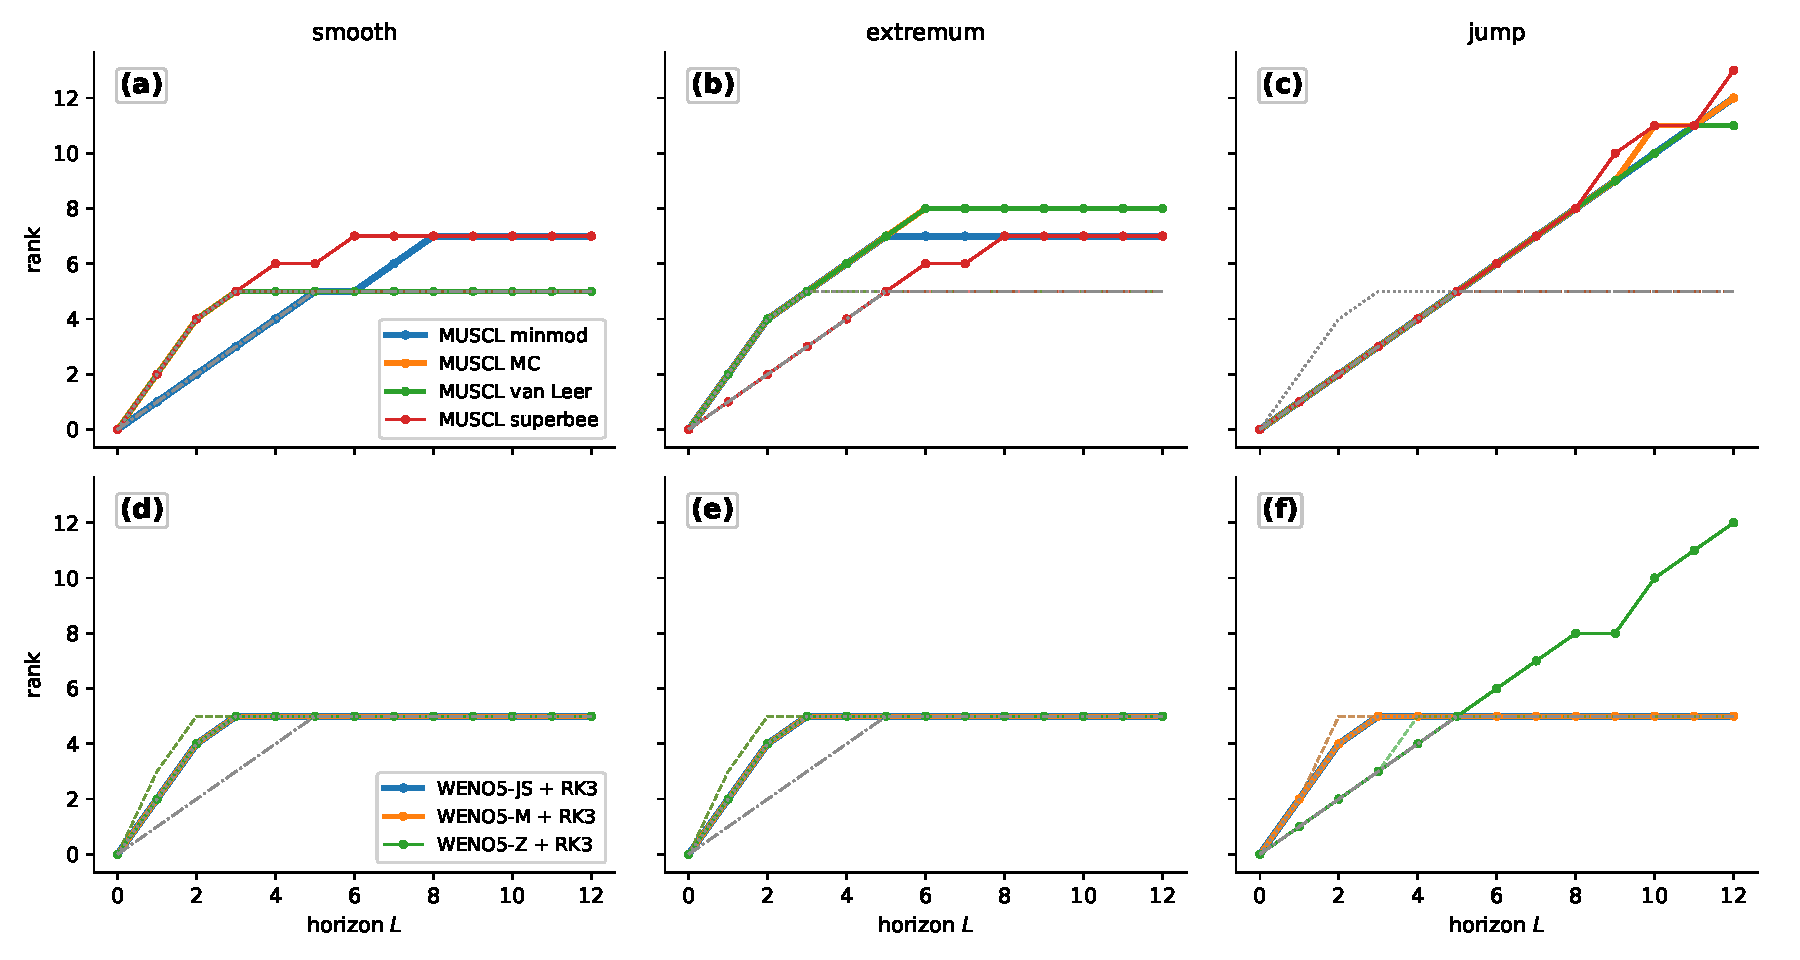
\includegraphics[width=\textwidth]{figures/nonlinear_rank_ladders.pdf}
\caption{E6: empirical response-span (solid, $\varepsilon=10^{-5}$, floor $\theta=10^{-3}$) and linearized (dashed) local ladders in the three base-state regimes, for the MUSCL family (top row) and the WENO5 family (bottom row): \textbf{(a)}~MUSCL, smooth; \textbf{(b)}~MUSCL, extremum; \textbf{(c)}~MUSCL, jump; \textbf{(d)}~WENO5, smooth; \textbf{(e)}~WENO5, extremum; \textbf{(f)}~WENO5, jump.
Gray references (Jacobian-response baselines): the two-collar law $\min(2L,r-1)$ (dotted) and the one-collar law $\min(L,r-1)$ (dash-dotted).
Smooth regime: minmod follows $\sigma=1$, the other limiters $\sigma=2$; at the extremum, the minmod and superbee roles swap.
Jump regime: all MUSCL linearizations collapse to UW1 ($\sigma=1$), while the response-span ladders continue past the linear budget $r-1=5$ at one direction per step.
In panels~(d) and~(e), the three WENO5 variants coincide exactly and are drawn with nested line widths so each stays visible; the mechanism and its significance are discussed in \cref{sec:exp-nonlinear}.}
\label{fig:nonlinear-ladders}
\end{figure}

\subsection{E7: flux-closure sanity check}\label{sec:exp-sanity}

E7 verifies, per scheme, the one-step telescoping identity underlying the realized-flux register, in the physical-flux normalization of \cref{rem:flux-normalization}: at the fine level, that the update is reproduced by its conservation form $u^{n+1}_i=u^n_i-\lambda(F_{i+1/2}-F_{i-1/2})$ --- with $F=\phi/\lambda$ the rescaled unique compact flux of \cref{prop:flux-form} for the linear family (constructed by partial summation in \texttt{schemes.py}) and the realized stage-summed flux $F=\tfrac16(F(u)+F(u^{(1)})+4F(u^{(2)}))$ for the SSP-RK3 pairings --- and at the coarse level, that every parent-average update equals $-(\lambda/r)$ times the difference of the two parent-interface physical fluxes, i.e.\ $-(1/r)$ times the compact-flux difference $B\Phi_t$ of \cref{prop:flux-form}, so the multi-point traces entering the parent-interface register close the coarse dynamics exactly, as in \cite{PolemitisChristakisDrikakis2026FVerasure}.
Across $96$ linear cases (all seven schemes plus the WENO5L + SSP-RK3 pairing, $r\in\{6,8\}$, the full $\lambda$ grid) and $63$ nonlinear cases (all seven MUSCL/WENO schemes on noisy smooth, discontinuous, and random data at $\lambda\in\{0.9,0.5,0.1\}$), the largest residual is $1.1\times10^{-15}$ at the fine level and $4.4\times10^{-16}$ at the coarse level (\texttt{flux\_closure.csv}): the closure identity holds to machine precision for every member of the family.

E7b verifies the saturated autonomous state of \cref{cor:coarse-recurrence}: for each linear scheme and the SSP-RK3 pairing, a random fine state is evolved and each coarse Fourier mode is tested against the depth-$r$ recurrence with characteristic polynomial $\prod_j(z-g_{m+jP})$, over $24$ post-saturation steps at $r\in\{6,8\}$ and $\lambda\in\{0.9,0.5,0.1\}$.
All $48$ cases satisfy the recurrence to machine precision (normalized residuals below $5\times10^{-15}$ for every stable pairing; the unstable WENO5-LIN + FE reaches $5\times10^{-12}$ only because its growing trajectory amplifies roundoff; \texttt{coarse\_recurrence.csv}).

%% =====================================================================
\section{Discussion}\label{sec:discussion}
%% =====================================================================

The starting point of this paper was a natural expectation: a scheme that transports information from $w$ cells per step should expose unresolved subcell data to the coarse observer faster than one that reads a single upstream neighbor.
\Cref{thm:rank-universal} refutes this at the level of dimension.
The exact memory requirement of coarse prediction is a rigidity property of the coarse/fine hierarchy itself --- $r$ fine modes alias onto each coarse mode, and each additional observation can separate at most one new node per residue class --- so every consistent circulant scheme outside the (certified empty) collision set climbs the same ladder, saturates at the same horizon, hides the same invisible subspace, and, by \cref{cor:coarse-recurrence}, closes on an autonomous register of the same depth.
Formal order, stencil reach, and dissipative order move none of these objects; the scheme survives only in the recurrence \emph{coefficients}, so the two remaining notions --- stable observability and dissipative erasure --- carry \emph{all} of the scheme dependence.
Universality is a statement about \emph{centralized} memory --- the dimension of a single global real-coordinate register --- and does not extend to the local communication picture: the per-parent encoder budgets of \cref{prop:local-encoder} remain scheme-dependent.

Timing is the first place the scheme reappears, and in the single-parent regime ($Lw\le r-1$), it obeys a counting rule of its own: collars, not width.
The per-parent exposure rate is $\sigma\in\{1,2\}$ (\cref{prop:local-rank}) no matter how many cells the stencil reads, while stencil \emph{reach} controls how soon deeply buried data first crosses an interface (\cref{cor:detection-delay}).
Once a single composed step spans several parents, the collar rule gives way to the wrap-around bound; the reach-$15$ WENO5--SSP-RK3 update exposes three directions in its first step (E1c).
The worst-case global delay $r-1$ is again universal, but the prescribed deepest pairs separate the schemes: in E5, first-order upwind geometrically shields the constructed two-cell perturbation for five steps, the second-order pairs for two, the wide stencils for at most one, and the composed WENO5--SSP-RK3 update for none at $r=6$; complete local detection follows by $T_{\rm loc}\le5$ steps in every case ($5$ for UW1 down to $2$ for the composed update; \cref{tab:half-life}).
Within the tested family, wider effective reach shortens the geometric shielding time of the prescribed localized perturbations, but it does not accelerate the global observation-rank ladder.

Recoverability is where scheme choice matters most given a fixed memory dimension.
The conditioning of delayed information is set by the exposure depth, $\sigma^{+}_{\min}({\cal O}_{L_q}\iota_K)\asymp\lambda^{L_q}$ (\cref{conj:conditioning} --- conjectured on the single-parent observation map for single-stage operators, supported within $0.05$ in every fitted exponent by E3), so a second collar halves the exponent: under this law, recovering the deepest saturated direction costs a tolerance of $\lambda^{3}$ for every two-collar single-stage scheme against $\lambda^{5}$ for first-order upwind --- four orders of magnitude of headroom at $\lambda=10^{-2}$.
The effective-rank ordering of E1 is the same phenomenon seen from above: Beam--Warming holds the full saturated rank at $\lambda=10^{-2}$, while Lax--Wendroff has already lost seven dimensions, although both share the exact ladder.
E2 traces the dichotomy to first-order node geometry --- LW's purely imaginary node velocity collapses a class gap to $\sqrt3\,\lambda^2$ (measured $1.73\times10^{-4}$ at $\lambda=10^{-2}$), a loss repaired by none of the horizons tested and requiring far longer observation windows than first-order separation (\cref{rem:gramian}), whereas BW's injective node map keeps every class separated at first order.
The warning of \cite{PolemitisChristakisDrikakis2026FVerasure} --- exact dimension should never be reported without its conditioning --- applies with more force across the hierarchy: the universal ladder makes schemes look identical exactly where they differ by orders of magnitude.

Relevance --- how long unresolved information stays dynamically alive --- completes the inversion of the naive picture.
The erasure hierarchy is $1-\rho_N=\tfrac12A(\lambda)(2\pi/N)^{2s}(1+o(1))$ with closed-form $A(\lambda)$ for every member (\cref{prop:dissipation,prop:interior-stability}), so retention scales as $N^{2s}$ in time steps ($N^{2s-1}$ in physical time): at $N=48$ and $\lambda=\tfrac12$ the information half-life runs from $3.2\times10^2$ steps for first-order upwind to $2.8\times10^7$ for UB5 --- a factor of $87{,}490$, nearly five orders of magnitude, between schemes with \emph{identical} memory dimension (\cref{tab:half-life}).
This is the revised penalty (\cref{rem:double-penalty}): the analyzed less-dissipative operators do not need more centralized closure information --- they keep the closure problem \emph{alive} longer.
The fully discrete pairing matters here: forward Euler destabilizes the fifth-order flux outright, and SSP-RK3 rescues it only by contributing integrator dissipation ($A=\lambda^4/12$, order $2s=4$) that overrides the sixth-order spatial decay (\cref{prop:weno-fe}) --- erasure claims are properties of scheme--integrator pairs, not of reconstructions (cf.\ \cite{PolemitisChristakisDrikakis2026onestep}).

For limited schemes, the linear taxonomy becomes a local dictionary rather than a restriction.
By \cref{prop:active-branch}, on piecewise-affine limiter branches the collision dynamics is \emph{exactly} that of one of the linear blends while the trajectory remains on a common branch, computable cell-by-cell from the active branch: minmod is one-collar precisely where its ratio sits on the $\varphi=\rho$ branch, superbee on the complementary slopes, and the roles swap between monotone and extremal data --- as E6 measures step for step.
On smooth non-affine arcs (van Leer at positive ratios), the tangent-line blend of \cref{rem:tangent-blend} describes only the local Jacobian response, which varies continuously with the slope ratio: there the dictionary is first-order, not exact.
The two genuinely nonlinear effects lie outside every linear budget.
Across the tested plateau ensembles, tolerances, and amplitude range ($10^{-7}\le\varepsilon\le10^{-2}$), the positively homogeneous dynamics widens the span of coarse responses by approximately one direction per step \emph{past} saturation: the span outgrows the Jacobian image and every linear budget --- a response-span effect, to be read as richness of the output map, not as additional state coordinates, and an empirical regularity rather than a proved law (\cref{sec:limitations}).
And the WENO regularization constant $\epsilon_w$ acts as an observability-regime threshold, not a numerical detail: it sets the perturbation amplitude below which the scheme is effectively linear at declared tolerance, while WENO-Z's scale-invariant weights keep it nonlinear at every tested amplitude (its own crossover, $\sqrt{\epsilon_Z}\approx10^{-20}$, lies far below them) and it inherits the staircase.
A validation protocol for nonlinear coarse prediction must therefore sample base states across the branch map: smooth, extremal, and plateau regimes respond with different collar counts, detection times, and nonlinear channels.

For coarse-grained and learned CFD models \cite{BarSinai2019,KochkovEtAl2021}, the practical takeaway is that the interesting benchmark quantities are not dimension counts.
Any claim of the form ``the coarse state plus $k$ centrally pooled features suffices'' transfers across the entire linear hierarchy, because the required $k$ is universal; what does \emph{not} transfer is when those features become visible, at what tolerance they are recoverable, and for how long they matter --- quantities that vary across schemes by factors of $10^2$ to $10^5$ at fixed resolution.
In particular, the information content of the training data depends strongly on the generating scheme: subcell signatures persist tens of thousands of times longer in data produced by a fifth-order method than by first-order upwind at the same $N$ (\cref{tab:half-life}).
These results suggest that a closure trained on data generated by a less-dissipative scheme may exhibit a longer effective-memory horizon --- a hypothesis about the training problem, not a result of this paper: no learned closure is studied here.
The declared-tolerance methodology of \cite{PolemitisChristakisDrikakis2026FVerasure, PolemitisChristakisDrikakis2026onestep}, which specifies the information set, the horizon, the tolerance, the scheme--integrator pair, and the error criterion, extends unchanged to the full hierarchy.
Experiments E7 and E7b confirm that its supporting register constructions (conservation-form fluxes, depth-$r$ recurrences) hold family-wide to machine precision.
The one addition this paper forces is that the \emph{scheme} is not an implementation detail of such a declaration: it is the quantity that moves every non-universal number in it.

%% =====================================================================
\section{Limitations and future work}\label{sec:limitations}
%% =====================================================================

\paragraph{Scope of the model.}
The analytical core is deliberately narrow: scalar linear advection on a uniform periodic one-dimensional grid, an integer coarsening ratio $r$, and translation-invariant (circulant) schemes.
Every structural result --- the universality theorem, the invisible subspace, the coarse recurrence, the dissipation ladder --- leans on Fourier block-diagonalization, and none of it transfers verbatim to nonuniform grids, nonperiodic boundaries, nonlinear conservation laws, or systems.
The nonlinear results of \cref{sec:nonlinear} are empirical: they characterize three base-state regimes of seven MUSCL/WENO schemes at one Courant number, anchored by \cref{prop:active-branch}, where limiter branches are affine, but they do not constitute a theory of limited schemes; the WENO smoothness indicators in particular are studied numerically, not analytically.
Time integration is forward Euler, except where stability requires SSP-RK3; thus, integrator effects enter only through that single pairing.
The encoder lower bounds are topological statements about continuous real-valued encoders (invariance of domain), not bit-complexity or statistical-learning bounds --- the same caveats as in \cite{PolemitisChristakisDrikakis2026FVerasure}.

\paragraph{Proof status.}
Several statements used or tested here remain conjectures or computer-assisted exact certificates rather than hand proofs, and are flagged as such in the text.
\begin{enumerate}
\item[(i)] The intermediate local rank law: the wrap-around upper bound is proved (\cref{lem:local-upper}), but its \emph{attainment} (\cref{conj:local-rank}) --- independence of the crossing functionals across parent boundaries --- is verified only numerically (exactly, at $r\in\{6,8\}$, E1c).
\item[(ii)] The conditioning law $\sigma^{+}_{\min}({\cal O}_{L_q}\iota_K)\asymp\lambda^{L_q}$ for the single-stage operators (\cref{conj:conditioning}; equivalent to the collar-to-queue form within the single-parent window $L_qw\le r-1$) is supported to within $0.05$ in every fitted exponent (E3), but a two-sided proof needs quantitative singular-value bounds along the $\lambda$-order filtration of \cref{rem:lambda-orders}.
      It does not extend unchanged to multistage operators: for the WENO5-LIN + SSP-RK3 pairing, the exact local rank counts directions before they appear at the corresponding power of $\lambda$ ($\sigma^{+}_{\min}({\cal O}_1\iota_K)=O(\lambda^{3})$ with $L_3=1$, \cref{conj:conditioning}), and a conditioning law for multistage operators belongs to the time-integration study proposed under future work below.
\item[(iii)] The collision-set emptiness certificate is analytic and grid-independent for UW1/LW/BW (\cref{prop:collision-empty}); for the wider stencils and the composed WENO5-LIN + SSP-RK3 pairing, it is an exact rational-arithmetic computation (\cref{prop:collision-certificate}, E1b) --- computer-assisted, without floating-point step --- but specific to the grid pairs examined, $(P,r)\in\{(8,6),(8,8)\}$.
      A grid-parameterized certificate, or a hand proof in the style of \cref{prop:collision-empty}, remains open.
\item[(iv)] Strict interior stability is proved in closed form for the six flux-form members (\cref{prop:interior-stability}) and by the exact two-region Bernstein certificate of \cref{prop:rk3-stability} for the WENO5-LIN + SSP-RK3 pairing, covering every $\lambda\in(0,1]$; the latter is computer-assisted (exact rational arithmetic), not a hand proof.
\item[(v)] The plateau response-span staircase $\rho^{\rm emp}(L)=L$ is an empirical law; the response-span (secant-span) dimension of positively homogeneous piecewise-linear dynamics is, to our knowledge, an open question.
\item[(vi)] \Cref{prop:active-branch} is exact only on affine limiter branches; smooth non-affine arcs (among the limiters used here: van Leer at positive ratios) are covered only to first order by the tangent-line blend of \cref{rem:tangent-blend}, and branch-boundary (kink) ratios by neither statement.
      Minmod, MC, and superbee are piecewise-affine and are therefore covered exactly at generic ratios.
\end{enumerate}

\paragraph{Limitations of the numerical tests.}
The grids are modest ($P=8$, $r\in\{6,8\}$; $N\le384$ for the erasure sweeps), chosen so that every observation matrix admits an exact dense SVD; the theorems are grid-general, but the conditioning and effective-rank findings are demonstrated at these sizes rather than swept to scale.
E6 fixes $\lambda=\tfrac12$ (the limiter branch structure is $\lambda$-independent, but detection prefactors and gap magnitudes were not swept), uses $M=400$ directions at two amplitudes and three base states, and its linearized reference is a finite-difference Jacobian with declared blind spots at limiter kinks and on plateaus; the rank floor, ensemble size, seed, FD step, and amplitude are, however, swept one at a time around this baseline in the Supplementary Material (Sec.~S2): the methodological knobs are inert, and only the declared floor and the physical amplitude move ranks, in the directions the crossover and gap analysis predicts.
The E5 tail fits are pre-asymptotic for $2s\ge6$; the predicted half-lives rest instead on $\rho_N$, which E4d verifies to machine precision.
Finally, every rank, detection, and recovery statement is tolerance-relative by construction --- declared SVD floors and separation thresholds --- which is the methodology of \cite{PolemitisChristakisDrikakis2026FVerasure, PolemitisChristakisDrikakis2026onestep}, but it means that no number in this paper should be quoted without its tolerance.

\paragraph{Future work.}
The gaps above define one track of future work: proving attainment of the wrap-around bound and the conditioning asymptotics; extending the exact collision certificate (iii) from the working grid pairs to parameterized $(P,r)$; a theory for the plateau staircase; and, on the numerical side, Courant and amplitude sweeps with richer base states for the nonlinear campaign.
Beyond repair work, three extensions naturally follow from what was found here.
First --- and in our view next --- a systematic study of \emph{time-integration information depth}: this paper ran into the integrator at every turn (forward Euler destabilizes the fifth-order flux; SSP-RK3's $\lambda^4/12$ overrides the spatial dissipative order; the realized flux register is stage-summed), and a dedicated taxonomy --- multistage trace depth for $s$-stage Runge--Kutta with per-stage reach $w$, multistep history as a separate memory channel, implicit solves trading detection delay for conditioning --- would complete the scheme--integrator picture that \cref{prop:weno-fe} opens, extending the one-step analysis of \cite{PolemitisChristakisDrikakis2026onestep} and reusing the exact symbol-polynomial machinery of this paper unchanged.
Second, a Riemann-solver taxonomy for nonlinear conservation laws: the collision-ensemble methodology of \cref{sec:nonlinear} transfers as-is to Burgers-type problems with Godunov, Roe, or HLL-family fluxes, where it can separate the destruction of physical information at shocks from numerical erasure.
Third, enriched coarse states: the universality theorem gives this classical question a new force, since scheme choice cannot accelerate the exposure ladder; the only lever on the memory dimension itself is enriching the coarse state (DG moments, interface point values), and the natural target is the self-predictivity threshold --- the smallest enriched state that is autonomous.
A scoped characteristic-variable Euler pilot, in which the linearized system decouples into advection fields with distinct effective Courant numbers, would be the first step toward systems.

%% =====================================================================
\section{Conclusions}\label{sec:conc}
%% =====================================================================

The exact centralized memory required for coarse finite-volume prediction does not depend on the scheme.
For every consistent member of the studied linear circulant family, outside a spectral-collision set that is provably finite and certified empty in exact rational arithmetic for all eight fully discrete operators and both grid pairs examined, the finite-horizon observation rank is \[ \rank\OL=P+(P-1)\min\{L,\,r-1\}, \] the first-order upwind ladder.
The saturation horizon $r-1$, the $(r-1)$-dimensional invisible subspace of repeated zero-mean profiles, and the depth-$r$ autonomous coarse recurrence are equally universal; formal order and stencil reach enter only through the recurrence coefficients.
The layer-counting intuition that wider stencils expose subcell memory faster is false --- it already violates the observation row bound.

Scheme dependence persists, concentrated along three axes that the dimension count cannot capture.
\emph{Timing}: in the single-parent regime information leaves a parent through its active collars, $\sigma\in\{1,2\}$, never faster --- though one composed step spanning several parents can expose more, as the reach-$15$ WENO5--SSP-RK3 update does --- while stencil reach sharply sets the geometric shielding time of the deepest prescribed perturbations: five shielded steps for first-order upwind against zero for that composed update at $r=6$, with complete local detection by $T_{\rm loc}\le r-1$ for every scheme.
\emph{Recoverability}: in a conjectured law for single-stage operators, supported by every fitted exponent (E3), the conditioning of delayed information scales as $\lambda^{L_q}$ with the exposure depth, so a second collar halves the exponent, and first-order node geometry --- not order --- decides which schemes lose effective rank at small Courant number.
\emph{Relevance}: the erasure hierarchy $1-\rho_N=\tfrac12A(\lambda)(2\pi/N)^{2s}(1+o(1))$, with closed-form leading coefficients for every member, spreads the information half-life across nearly five orders of magnitude at fixed resolution, and the fully discrete dissipative order belongs to the scheme--integrator pair (\cref{prop:weno-fe}).

Together, these results replace the expected \enquote{double penalty} of high order with a sharper, more conditional statement.
Across the collision-free linear hierarchy, the centralized memory dimension is invariant, while local communication budgets stay scheme-dependent (\cref{prop:local-encoder}).
Formal order itself guarantees neither earlier detection nor friendlier recovery: wider \emph{effective reach} shortens the geometric shielding time of prescribed perturbations, and additional \emph{active collars} improve local depth conditioning --- but Beam--Warming is second order with a single active collar, and Lax--Wendroff loses effective rank before first-order upwind at small Courant number through its class-node degeneracy, so global recoverability can deteriorate even as formal order rises.
At the declared resolution, the analyzed less-dissipative operators retain unresolved signatures orders of magnitude longer at the same centralized memory dimension: the dissipation that would otherwise retire unresolved information is precisely the error they are built to remove.

For limited schemes, observability becomes state-dependent in an enumerable way: on every affine limiter branch, the MUSCL flux is exactly a linear blend --- on smooth non-affine arcs, only its Jacobian is --- so the active branch, not the nominal stencil, sets the local exposure rate, as the ensemble experiments confirm branch by branch.
Two effects are genuinely nonlinear: across the tested plateau ensembles, tolerances, and amplitudes, the response-span rank grows approximately one direction per step \emph{beyond} the linear budget --- a secant-span effect rather than additional state, and an empirical regularity still awaiting proof --- and the WENO regularization constant is the amplitude threshold below which the scheme is effectively linear at declared tolerance (WENO-Z, nonlinear at every tested amplitude, makes the contrast visible).

The practical lesson extends the declaration protocol of \cite{PolemitisChristakisDrikakis2026FVerasure, PolemitisChristakisDrikakis2026onestep} by one clause.
A meaningful claim about coarse prediction must declare the information set, the horizon, the tolerance, the error criterion, and the scheme--integrator pair, because the centralized dimension is the only quantity invariant across the hierarchy.
The three questions --- what is the exact predictive state, how well conditioned is it, and which parts survive dissipation --- now have family-wide answers for linear reconstructions on the periodic scalar hierarchy, empirical answers for their limited and WENO counterparts, and a clearly marked next frontier in the time integrator.

%% =====================================================================
\section*{Declarations}

\subsection*{Funding}
No external funding was received for this work.

\subsection*{Competing interests}
The authors declare that they have no financial or non-financial interests that are directly or indirectly related to the work submitted for publication.

\subsection*{Author contributions}
A.P. contributed to conceptualization, interpretation, verification, and writing.
I.K. contributed to numerical analysis, software, interpretation, verification, and writing.
N.C. contributed to conceptualization, mathematical analysis, numerical analysis, interpretation, verification, and writing.
D.D. contributed to conceptualization, numerical analysis, interpretation, verification, and writing.
All authors reviewed and approved the manuscript.

\section*{Acknowledgments}

The authors used generative AI tools in the course of this work for literature discovery, drafting assistance with the text and with the experiment and verification code, adversarial review of the mathematical arguments, and copyediting suggestions.
The research questions, results, and conclusions are the authors' own.
The authors verified all cited sources, mathematical arguments, numerical results, and the final text, and assume responsibility for all content.

\section*{Data and code availability}

The complete reproducibility package for this study is publicly available in the Certified Simulation repository of the University of Nicosia, \url{https://github.com/UniversityOfNicosia/certified-simulation}, under \texttt{papers/coarse-observability-high-order}, as the frozen release tagged \texttt{coarse-observability-high-order-v1}.
The package contains the Python scripts that generate every rank ladder, singular-value table, conditioning fit, erasure experiment, nonlinear ensemble, sensitivity sweep, CSV file, LaTeX table fragment, and figure reported in the manuscript, executable certificates that replay the paper's exact results (collision-set emptiness, interior stability of the SSP-RK3 pairing) in exact rational arithmetic, and instructions for reproducing the results.
The only dependencies are Python, NumPy, and Matplotlib; no external CFD solver or proprietary software is required.

\section*{Supplementary information}

The Supplementary Material accompanying this article contains the exact coefficient polynomials of the composed WENO5-LIN + SSP-RK3 one-step operator (Sec.~S1, Table~S1) and the full one-at-a-time sensitivity analysis of the nonlinear ranks (Sec.~S2, Table~S2), both machine-generated by \texttt{make\_tables.py} from the same exact representations and CSV artifacts as the in-article tables.

%% =====================================================================
\begin{appendices}
\counterwithin*{table}{section}% restart table numbers in each appendix

\section{Explicit coefficients and stencils}\label{app:coefficients}

Every coefficient in this appendix --- and in Table~S1 of the Supplementary Material --- is generated by \texttt{make\_tables.py} from the exact rational-arithmetic representations in \texttt{schemes.py} (\texttt{coeff\_polys}, \texttt{weno5l\_rk3\_polys}); no coefficient is transcribed by hand (machine-generated fragment: \texttt{results/tables/coefficients.tex}).

\subsection{Semi-Lagrangian members and their interpolation nodes}
\label{app:sl-coefficients}

UW1, LW, BW, UB3, and UB5 are Lagrange interpolation schemes: with integer node set $D\subset\mathbb Z$ (offsets relative to cell $i$), the update interpolates the previous state at the departure offset $-\lambda$, \[ c_{-d}(\lambda)=\prod_{d'\in D\setminus\{d\}} \frac{-\lambda-d'}{d-d'},\qquad d\in D, \] so the coefficient of $u_{i-s}$ is $c_s$ with $s=-d$.
The node sets are \[ D_{\rm UW1}=\{-1,0\},\quad D_{\rm LW}=\{-1,0,1\},\quad D_{\rm BW}=\{-2,-1,0\}, \] \[ D_{\rm UB3}=\{-2,-1,0,1\},\quad D_{\rm UB5}=\{-3,-2,-1,0,1,2\}, \] and FR is the arithmetic mean of LW and BW (\cref{sec:linear-family}).
\Cref{tab:coeff-sl} lists the expanded coefficient polynomials.
Each Lagrange coefficient is, up to a rational constant, the product $\prod_{d'\in D\setminus\{d\}} (\lambda+d')$, and FR's four coefficients factor likewise (e.g.\ $c_0=(\lambda+4)(1-\lambda)/4$); no factor has a root in the open interval $(0,1)$, which is the root structure used in \cref{rem:effective-support}.

\begin{table}[htbp]
\centering
\caption{Exact coefficient polynomials $c_s(\lambda)$ of the semi-Lagrangian members and Fromm (update $u_i^{n+1}=\sum_s c_s(\lambda)\,u_{i-s}^n$).}
\label{tab:coeff-sl}
\begin{tabular}{@{}lrl@{}}
\toprule
Scheme & $s$  & $c_s(\lambda)$                                                                                                                      \\
\midrule
UW1    & $1$  & $\lambda$                                                                                                                           \\
       & $0$  & $1 - \lambda$                                                                                                                       \\
\midrule
LW     & $1$  & $\tfrac{1}{2}\lambda + \tfrac{1}{2}\lambda^{2}$                                                                                     \\
       & $0$  & $1 - \lambda^{2}$                                                                                                                   \\
       & $-1$ & $-\tfrac{1}{2}\lambda + \tfrac{1}{2}\lambda^{2}$                                                                                    \\
\midrule
BW     & $2$  & $-\tfrac{1}{2}\lambda + \tfrac{1}{2}\lambda^{2}$                                                                                    \\
       & $1$  & $2\lambda - \lambda^{2}$                                                                                                            \\
       & $0$  & $1 - \tfrac{3}{2}\lambda + \tfrac{1}{2}\lambda^{2}$                                                                                 \\
\midrule
FR     & $2$  & $-\tfrac{1}{4}\lambda + \tfrac{1}{4}\lambda^{2}$                                                                                    \\
       & $1$  & $\tfrac{5}{4}\lambda - \tfrac{1}{4}\lambda^{2}$                                                                                     \\
       & $0$  & $1 - \tfrac{3}{4}\lambda - \tfrac{1}{4}\lambda^{2}$                                                                                 \\
       & $-1$ & $-\tfrac{1}{4}\lambda + \tfrac{1}{4}\lambda^{2}$                                                                                    \\
\midrule
UB3    & $2$  & $-\tfrac{1}{6}\lambda + \tfrac{1}{6}\lambda^{3}$                                                                                    \\
       & $1$  & $\lambda + \tfrac{1}{2}\lambda^{2} - \tfrac{1}{2}\lambda^{3}$                                                                       \\
       & $0$  & $1 - \tfrac{1}{2}\lambda - \lambda^{2} + \tfrac{1}{2}\lambda^{3}$                                                                   \\
       & $-1$ & $-\tfrac{1}{3}\lambda + \tfrac{1}{2}\lambda^{2} - \tfrac{1}{6}\lambda^{3}$                                                          \\
\midrule
UB5    & $3$  & $\tfrac{1}{30}\lambda - \tfrac{1}{24}\lambda^{3} + \tfrac{1}{120}\lambda^{5}$                                                       \\
       & $2$  & $-\tfrac{1}{4}\lambda - \tfrac{1}{24}\lambda^{2} + \tfrac{7}{24}\lambda^{3} + \tfrac{1}{24}\lambda^{4} - \tfrac{1}{24}\lambda^{5}$  \\
       & $1$  & $\lambda + \tfrac{2}{3}\lambda^{2} - \tfrac{7}{12}\lambda^{3} - \tfrac{1}{6}\lambda^{4} + \tfrac{1}{12}\lambda^{5}$                 \\
       & $0$  & $1 - \tfrac{1}{3}\lambda - \tfrac{5}{4}\lambda^{2} + \tfrac{5}{12}\lambda^{3} + \tfrac{1}{4}\lambda^{4} - \tfrac{1}{12}\lambda^{5}$ \\
       & $-1$ & $-\tfrac{1}{2}\lambda + \tfrac{2}{3}\lambda^{2} - \tfrac{1}{24}\lambda^{3} - \tfrac{1}{6}\lambda^{4} + \tfrac{1}{24}\lambda^{5}$    \\
       & $-2$ & $\tfrac{1}{20}\lambda - \tfrac{1}{24}\lambda^{2} - \tfrac{1}{24}\lambda^{3} + \tfrac{1}{24}\lambda^{4} - \tfrac{1}{120}\lambda^{5}$ \\
\bottomrule
\end{tabular}
\end{table}

\subsection{Linear WENO5: interface flux and flux-difference operator}
\label{app:weno-coefficients}

With the linear weights $(d_0,d_1,d_2)=(\tfrac1{10},\tfrac6{10},\tfrac3{10})$ the upwind-biased fifth-order interface flux is \[ \hat f_{i+1/2} =\frac{2u_{i-2}-13u_{i-1}+47u_{i}+27u_{i+1}-3u_{i+2}}{60}, \] and the forward-Euler update $u_i^{n+1}=u_i-\lambda\bigl(\hat f_{i+1/2}-\hat f_{i-1/2}\bigr)$ is the circulant operator with support $s\in\{-2,\dots,3\}$, $(m_L,m_R)=(3,2)$, and affine coefficients
\begin{gather*}
c_{3}=\tfrac{1}{30}\lambda,\quad
c_{2}=-\tfrac{1}{4}\lambda,\quad
c_{1}=\lambda,\\
c_{0}=1 - \tfrac{1}{3}\lambda,\quad
c_{-1}=-\tfrac{1}{2}\lambda,\quad
c_{-2}=\tfrac{1}{20}\lambda .
\end{gather*}

\end{appendices}

\bibliography{article}

\end{document}
